%CD=15
%CP=40
%PR=25
%IE=5
%P=15

\setcounter{secnumdepth}{0}
\setcounter{tocdepth}{1}

\newcounter{ns}
\addtocounter{ns}{1}

\newcounter{re}
\addtocounter{re}{1}
\setcounter{re}{1}

\newcounter{su}
\addtocounter{su}{1}

\newcounter{par}
\addtocounter{par}{1}


\newpage

\definecolor{istat}{RGB}{0,50,100}
\begin{center}
\textbf{\textcolor{istat}{INSTITUTO DE EDUCACIÓN SUPERIOR TECNOLÓGICO PRIVADO “ADVENTISTA DEL TITICACA”}}
\end{center}

\begin{center}
\textbf{\textcolor{istat}{REGLAMENTO INTERNO}}
\end{center}
%----------------------------------------------------------------------------------------
%\renewcommand{\partname}{TÍTULO}
%\renewcommand{\thesection}{CAPÍTULO \Roman{section}}
%\renewcommand{\thesubsection}{Artículo \arabic{subsection}}

\part{TÍTULO \Roman{par}. DEL INSTITUTO}
\addtocounter{ns}{1}
\section{CAPÍTULO \Roman{re}. DE LA IDENTIDAD, ORIGEN Y LA AUTONOMÍA }
\addtocounter{re}{1}
\subsection{Artículo \arabic{ns}. ISTAT: Identidad}
\addtocounter{ns}{1}
El Instituto Superior no Estatal “Adventista del Titicaca” (ISTAT), es una comunidad educativa dedicada a la formación profesional tecnológica del ámbito de la educación superior no universitaria, integrada por docentes, estudiantes y graduados. Es apolítico, con personería jurídica de derecho privado sin fines de lucro; orientada a la formación técnica y la innovación; brinda una formación integral del ser humano en sus dimensiones física, mental, social, espiritual y humanidades con una clara conciencia de su misión de servicio a la sociedad. 
\subsection{Artículo \arabic{ns}. ISTAT: Origen y Promotora}
\addtocounter{ns}{1}
El ISTAT fue promovido y creado por la Iglesia Adventista del Séptimo Día (antes: Asociación Unión Peruana de la Iglesia Adventista del Séptimo Día y, antes, Asociación Unión Incaica de la Iglesia Adventista del Séptimo Día), y por decisión de la misma, el 16 de abril de 2021 transfirió sus derechos de Promotoria a la UNIVERSIDAD PERUANA UNIÓN (UPeU) quien en razón de su naturaleza promociona, promueve y conduce al ISTAT como un centro universitario de prestación de servicios educativos de nivel de educación superior no universitario, conforme a las disposiciones vigentes.

El ISTAT legalmente es una persona jurídica de derecho privado, bajo la naturaleza jurídica asociativa, y no tiene fines de lucro. 
\subsection{Artículo \arabic{ns}. ISTAT: Carácter apolítico}
\addtocounter{ns}{1}
El ISTAT es apolítico, asumiendo en pleno y totalmente los preceptos estatutarios y reglamentarios declarados de su Promotora.
\subsection{Artículo \arabic{ns}. ISTAT: Domicilio}
\addtocounter{ns}{1}
El ISTAT tiene su domicilio legal en Carretera Arequipa Km. 6 – Villa Chullunquiani, distrito de Juliaca, provincia de San Román y departamento de Puno. 
El domicilio del ISTAT, conforme a las disposiciones de su Promotora, es:
\begin{enumerate}
\item El lugar donde funciona.
\item El creado para el cumplimiento de sus fines. Previa autorización de su Promotora.
\end{enumerate}
\subsection{Artículo \arabic{ns}. ISTAT: Uso de sigla, emblemas, signos distintivos y derechos de propiedad}
\addtocounter{ns}{1}
El ISTAT en el ejercicio de su potestad de gobierno, normativa y administrativa de sus bienes tangibles e intangibles, materiales e inmateriales, regula en aplicación de las normas de su Promotora, el uso, disposición o transferencia a título gratuito u oneroso, de sus signos distintivos, previa autorización expresa de la misma Promotora. 

En su funcionamiento regula la propiedad intelectual de los miembros de su comunidad a través de reglamentos específicos, en el marco de los de su Promotora.

\subsection{Artículo \arabic{ns}. Alcances}
\addtocounter{ns}{1}
El reglamento interno del ISTAT es de aplicación a todos los miembros de su comunidad educativa, sin más limitaciones que las establecidas por el mismo. Asimismo, en todo acto, situación o decisión de sus unidades académicas, de apoyo administrativo, financiero y de servicios en general.
\subsection{Artículo \arabic{ns}. Objeto del Reglamento}
\addtocounter{ns}{1}
Son objetivos del presente reglamento:
\begin{enumerate}
\item Definir y establecer las responsabilidades, atribuciones, funciones, relaciones internas y externas de los miembros de la comunidad educativa del ISTAT. 
\item Establecer los lineamientos y orientaciones institucionales en el marco de la Ley de Institutos y Escuelas de Educación Superior y de la Carrera Pública de sus Docentes.  
\item Orientar el desarrollo de las labores técnico pedagógicas, administrativas y de gestión promoviendo la mejora profesional y personal de la comunidad educativa.  
\item Facilitar el desarrollo de las funciones operativas y administrativas estableciendo las bases para el sistema de control y facilitar el control de las funciones delegadas. 
\item Establecer los lineamientos y las orientaciones para el desarrollo de los procesos de la enseñanza y aprendizaje
\end{enumerate}
\subsection{Artículo \arabic{ns}. Marco Normativo}
\addtocounter{ns}{1}
\begin{enumerate}
\item Constitución Política del Perú.
\item Ley Nº 28044, Ley General de Educación.
\item Ley Nº 30512, Ley de Institutos y Escuelas de Educación Superior y de la Carrera Pública de sus Docentes.
\item Resolución de Secretaría General Nº 178-2018-MINEDU Lineamientos Académicos Generales para los Institutos de Educación Superior
\item D.S. Nº 010-2017-MINEDU. Reglamento de la Ley N° 30512, Ley de Institutos y Escuelas de Educación Superior y de la Carrera Pública de sus Docentes.
\item Resolución de Secretaría General N° 322-2017 Condiciones básicas para el procedimiento de licenciamiento de los institutos de educación superior.
\item Ley Nº 26549, Ley de los Centros Educativos Privados.
\item Ley Nº 28340. Sistema de Información de Educación para el Trabajo.
\item Ley Nº 28740. Ley del Sistema Nacional de Evaluación, Acreditación y Certificación de la Calidad Educativa.
\item Decreto Ley N° 25762. Ley Orgánica del Sector Educación.
\item D.S. Nº 021-2006-ED. Lineamientos Nacionales de Política de la Formación Profesional.
\item R.V.M. 277-2019-MINEDU Modificatoria en los Lineamientos Académicos Generales para los institutos de educación superior y las escuelas de educación superior tecnológica.
\item DECRETO DE URGENCIA Nº 017-2020. Establece medidas para el fortalecimiento de la gestión y el licenciamiento de los institutos y escuelas de educación superior, en el marco de la ley nº 30512, ley de institutos y escuelas de educación superior y de la carrera pública de sus docentes.
\item Ley N° 23585 - Gobierno del Perú.
\item Decreto Legislativo Nº 1495, que establece disposiciones para garantizar la continuidad y calidad de la prestación del servicio educativo en los institutos y escuelas de educación superior, en el marco de la emergencia sanitaria causada por el COVID-19.
\item D.S. 016-2021-MINEDU, que modifica el reglamento de la Ley de Institutos y Escuelas de Educación Superior y de la Carrera Pública de sus docentes.
\end{enumerate}
\subsection{Artículo \arabic{ns}. ISTAT: De la autonomía}
\addtocounter{ns}{1}
El ISTAT tiene autonomía normativa, de gobierno, académica, económica, y administrativa. Está regida por la Constitución Política del Perú, Ley Nº 30512, Ley de Institutos y Escuelas de Educación Superior y de la Carrera Pública de sus Docentes, la legislación vigente del sector, su Reglamento Interno.  
Esta autonomía comprende las siguientes dimensiones: 
\begin{enumerate}
\item Normativa, implica la potestad del ISTAT para la creación de normas internas destinadas a su regulamiento, en concordancia con la filosofía de la educación adventista. 
\item De gobierno, implica la potestad autodeterminativa del ISTAT para estructurar, organizar y conducir, de acuerdo con su naturaleza, características y necesidades, en armonía con los principios de la promotora.  
\item Académica, implica la potestad autodeterminativa del ISTAT para fijar el marco del proceso de enseñanza y el aprendizaje dentro del Instituto Superior no Estatal “Adventista del Titicaca”. Así como formula, promueve, desarrolla y ejecuta planes, programas, proyectos, actividades en el programa de estudios, innovación, cultural, económica, social, artística, inclusión, medio ambiente y demás ámbitos del conocimiento y creación humana, según la filosofía de la educación adventista. 
\item Administrativa, implica la potestad autodeterminativa del ISTAT para establecer los principios, técnicas y prácticas de sistemas de gestión, tendientes a facilitar la consecución de los fines del Instituto Superior no Estatal “Adventista del Titicaca”.  
\item Económica, implica la potestad autodeterminativa del ISTAT para administrar y disponer del patrimonio institucional, así como para fijar los criterios de generación y aplicación de los recursos, con aprobación de la promotora, en armonía con los principios y las normas de la promotora.
\end{enumerate}
%----------------------------------------------------------------------------------------

\section{CAPÍTULO \Roman{re}. DE LOS FINES Y OBJETIVOS }
\addtocounter{re}{1}
\subsection{Artículo \arabic{ns}. Fines}
\addtocounter{ns}{1}

El ISTAT, conforme a su naturaleza, origen y propósitos de su Promotora, tiene por fines los siguientes:
\begin{enumerate}
\item Formar integralmente al ser humano, en sus aspectos físico, mental, espiritual y social, además cultivar los valores ético-cristianos, su responsabilidad y vocación de servicio a Dios, a la patria y a la humanidad.  
\item Formar profesionales técnicos de alta calidad, de acuerdo con su misión, las necesidades del país y los propósitos de su promotora.  
\item Realizar innovación, así como fomentar la creación intelectual y artística.  
\item Promover la conducta ético cristiana en sus estudiantes, docentes, personal no docente del Instituto. 
\end{enumerate}
\subsection{Artículo \arabic{ns}. Objetivos}
\addtocounter{ns}{1}
El modelo educativo del ISTAT tiene los siguientes objetivos:
\begin{enumerate}
\item Ofrecer a los estudiantes las condiciones propicias para el desarrollo de la innovación tecnológica, en las diversas áreas del conocimiento, propio de los programas de estudio.   
\item Utilizar estrategias metodológicas y técnicas para el desarrollo de las competencias propias del programa de estudios, así como, para la innovación y sus implicancias para lograr el perfil de egreso del estudiante.  
\item Conducir a los estudiantes a desarrollar una vida íntegra, teniendo como base principios compatibles con los valores éticos – cristianos, sociales y de servicio.  
\item Estimular la adquisición de la sabiduría, la evaluación crítica y reflexiva, el descubrimiento, la diseminación del conocimiento y el fortalecimiento y la puesta de práctica en favor de la comunidad en general.
\end{enumerate}
\subsection{Artículo \arabic{ns}. Articulación}
\addtocounter{ns}{1}
Los estudios realizados en el ISTAT, en los diferentes programas de estudio, se articulan con los de otros Institutos conforme a las necesidades del mercado laboral y del sector empresarial, y con las universidades que tenga convenio, por medio de la convalidación académica o la homologación de planes de estudio y competencias de los estudiantes o titulandos.
\subsection{Artículo \arabic{ns}. Cooperación}
\addtocounter{ns}{1}
El ISTAT promueve la cooperación con otros Institutos, Escuelas y Universidades, en los ámbitos nacional e internacional con fines de innovación, académicos, administrativos e institucionales en la realización de proyectos y programas de formación y difusión de experiencias formativas. 
 
El ISTAT promoverá e integrará la red educativa de intercambio de experiencias formativas técnico-profesionales, a nivel regional y macro-regional, en los aspectos académico, administrativo e institucional.
\section{CAPÍTULO \Roman{re}. DEL MARCO FILOSÓFICO, AXIOLÓGICO Y PROPÓSITOS }
\setcounter{re}{1}
\subsection{Artículo \arabic{ns}. Fundamento}
\addtocounter{ns}{1}
La filosofía de la educación cristiana adventista es la piedra angular en la planificación, desarrollo, implementación y evaluación de la actividad formativa, educativa, en los programas de estudios. 
\subsection{Artículo \arabic{ns}. Implicancias}
\addtocounter{ns}{1}
La filosofía de la educación adventista implica para el ISTAT: 
\begin{enumerate}
\item El compromiso y responsabilidad de sus autoridades en preservar el contexto educativo: enseñanza, aprendizaje, la recreación, la actividad deportiva, social, espiritual, cultural y otro ámbito del quehacer, bajo el marco de la educación cristiana bíblica adventista. 
\item La formulación, implementación, evaluación y reformulación sistemática de los programas, proyectos, planes, actividades y acciones consensuados, concertados, planificados y previsores de los escenarios educativos que fortalezcan la identidad filosófica y axiológica cristiana bíblico adventista. 
\item El accionar docente centrado en la formación del ser, la calidad y excelencia académica y el servicio hacia el prójimo, la humanidad y el país. 
\item La vida educativa esencial del estudiante, fundada y matizada transversalmente por la formación del carácter, del ser, como objetivo educacional y fin último, de la restauración de la imagen de Dios. 

\end{enumerate}
\subsection{Artículo \arabic{ns}. ISTAT: Cumplimiento del marco filosófico y axiológico}
\addtocounter{ns}{1}
En el quehacer académico, cualquiera sea su nivel o modalidad, los miembros de la comunidad del ISTAT observan, cumplen, cautelan, respetan y propician exprofesamente, de propósito, el cumplimiento de la filosofía de la educación cristiana adventista. Este mismo propósito y control comprende a sus direcciones y demás instancias administrativas, además de las funciones y roles de las unidades de apoyo, áreas administrativas y otras del ISTAT. 
\subsection{Artículo \arabic{ns}. ISTAT: Redes interinstitucionales}
\addtocounter{ns}{1}
El ISTAT en cumplimiento de sus propósitos, fines, objetivos y funciones promueve, participa y sostiene con sus capacidades y recursos en la organización, constitución, funcionamiento y desarrollo de redes interinstitucionales, organismos, corporaciones o instituciones educativas esencialmente de la red corporativa adventista mundial en el cumplimiento de su misión y la de su Promotora. Así como el sostenimiento, funcionamiento y desarrollo de redes interinstitucionales de cooperación académica, investigación e innovación o transferencia tecnológica, proyectos o programas en las líneas de acción definidas o convenidas. 
\subsection{Artículo \arabic{ns}. ISTAT: Operador de convenios}
\addtocounter{ns}{1}
Los convenios, acuerdos, cartas de intención o adendas están bajo la gestión en la suscripción de la oficina de Cooperación y Relaciones Nacionales e Internacionales y aprobados por el Consejo Administrativo. La gestión de su implementación corresponde según la naturaleza de los compromisos, programas, actividades o acciones a la unidad académica o de apoyo designada expresamente, bajo responsabilidad. 
\subsection{Artículo \arabic{ns}. Red de Educación Adventista}
\addtocounter{ns}{1}
El ISTAT es parte de la Universidad Peruana Unión y esta es parte de la Red de Educación Adventista, administrada por la Iglesia Adventista del Séptimo Día.
\subsection{Artículo \arabic{ns}. Filosofía}
\addtocounter{ns}{1}
La visión y misión del Instituto Superior no Estatal “Adventista del Titicaca” está basada sobre los principios de la filosofía educativa adventista con una concepción bíblico-cristiana. Toda actividad académica, administrativa, de producción y de prestación de servicios el ISTAT es desarrollada de acuerdo con los principios de la filosofía educativa de su promotora.
\subsection{Artículo \arabic{ns}. ISTAT: Implementación de la misión y visión}
\addtocounter{ns}{1}
La misión y visión institucional es difundida e implementada en todo el quehacer de la vida educativa. El ISTAT evalúa su cumplimiento sistemático, participativo, así como su revisión a través del marco normativo respectivo.
\subsection{Artículo \arabic{ns}. Visión}
\addtocounter{ns}{1}
“Ser referente en el mundo por el modelamiento de profesionales técnicos íntegros, misioneros e innovadores con un estilo de vida saludable”.
\subsection{Artículo \arabic{ns}. Misión}
\addtocounter{ns}{1}
“Somos una comunidad educativa dedicada a la formación profesional técnica de la Iglesia Adventista del Séptimo Día que modela personas a fin de que sean íntegras, misioneras e innovadoras basados en la cosmovisión bíblica-cristiana para servir a Dios y la humanidad”.
\subsection{Artículo \arabic{ns}. Principios}
\addtocounter{ns}{1}
El Instituto Superior no Estatal “Adventista del Titicaca”, además de los establecidos por ley, se rige por los siguientes principios:
\begin{enumerate}
\item Amor: Principio fundamental de una educación concebida como redentora. Implica el establecimiento de relaciones interpersonales profesor-estudiante que sean gratificantes y placenteras. 
\item Centralidad en las Sagradas Escrituras: Dios y su revelación escrita, la Biblia, son el centro de la educación. Esto significa que la visión bíblica del mundo y de la realidad constituyen la base del proceso de enseñanza-aprendizaje y la pauta orientadora del trabajo docente. Significa también que cada una de las materias de estudio, las artes, las letras, las ciencias, la historia, etc., son enfocadas desde la perspectiva bíblica. Significa que el objetivo más importante es el conocer a Dios y a Cristo como Salvador personal de cada uno de los componentes de la comunidad educativa. 
\item La semejanza a cristo: Uno de los grandes fines de la educación adventista es desarrollar la semejanza al carácter de Cristo. En consecuencia, el proceso formador otorga mayor importancia a la obtención de un carácter como el de Cristo que al tratamiento de las asignaturas, lo que hace que el ejemplo de los maestros, más que el proceso de instrucción, cobre vital importancia. De lo anterior se desprende que resulta indispensable crear un ambiente propicio para alcanzar dicho fin. 
\item El desarrollo armonioso: Concebimos a la educación como un proceso de desarrollo armonioso y equilibrado del ser humano en sus aspectos físico, intelectual, social y espiritual. Esto significa que en el proceso educativo no corresponde privilegiar ninguno de estos aspectos en desmedro de otros, sino que todos ellos deben ser atendidos por igual. 
\item La racionalidad: La educación adventista aspira a desarrollar los poderes de la mente y la capacidad de pensar y razonar. De ello se desprende que debe llevarse a cabo un proceso de enseñanza – aprendizaje de alta calidad, en que se estimulen la excelencia, el pensamiento reflexivo e independiente y la prosecución de metas altas, acordes con las capacidades personales. 
\item La individualidad: En nuestro proceso formador se considera al individuo como dotado de libre albedrío, capaz de tomar sus propias decisiones y de responsabilizarse por las consecuencias que le acarrean. Por ello, se fortalece el concepto de trabajo individual, aunque se desincentiva el espíritu de competencia, privilegiándose, en cambio, el sentido de interdependencia y cooperación. 
\item La salud: La educación adventista favorece el desarrollo de un cuerpo sano por medio del trabajo, fomenta el trabajo físico, el conocimiento del cuerpo humano, de las leyes de la salud y la prevención de las enfermedades mediante hábitos correctos de alimentación, horarios de trabajo y descanso apropiados, etc. 
\item El servicio: La educación adventista procura adiestrar para el servicio en favor de los demás. Se concede importancia a los deberes prácticos de la vida, se estimula una actitud permanente de servicio al prójimo y se incentiva la búsqueda de oportunidades de servir. 
\item La cooperación: Maestros y estudiantes deben de cooperar mutuamente. La cooperación es el esquema básico de trabajo, superando los criterios de competición. Cada estudiante debe recibir una educación que lo capacite para el servicio mediante el ejercicio activo de todas sus facultades. Se debe combinar el servicio con el entrenamiento. 
\item Continuo aprendizaje: La filosofía educacional adventista considera que el proceso educativo comienza desde el nacimiento mismo y continúa de manera permanente e indefinida a lo largo de todo el periodo de vida accesible al hombre.
\end{enumerate}
%-------------------------------------------------------------------------------
\part{TÍTULO \Roman{par}. DE LA PROMOTORA}
\addtocounter{ns}{1}
\subsection{Artículo \arabic{ns}. Promotora: Definición}
\addtocounter{ns}{1}
El ISTAT es un Centro Universitario de Prestaciones de Servicios Educativos, promovido, dirigido y bajo la gestión de su Promotora la Universidad Peruana Unión (UPeU). La Promotora tiene derechos intransmisibles, irrenunciables y plenos en todos los aspectos de la vida administrativa, académica y de gestión. 
\subsection{Artículo \arabic{ns}. Promotora: Prerrogativas específicas}
\addtocounter{ns}{1}
La Promotora, (UPeU) en uso de su potestad, autoridad y derechos de promotoría:
\begin{enumerate}
\item Disponer auditorias cotidianas o intempestivas a cualquiera de los niveles de gestión del ISTAT.
\item Crear comisiones o comités que fortalezcan o posibiliten la gestión del ISTAT con mayor eficiencia.
\item Establecer la reorganización, adscripción, cierre o cese de actividades por convenir a sus derechos.
\item Formular observaciones, reparos u otros en alguno o todos los asuntos, aspectos o actos dispuestos para su funcionamiento o gestión, cautelando la naturaleza y propósitos del ISTAT.
\item Formular planes, programas, proyectos o actividades y presentarlos a los órganos del ISTAT para su consideración e implementación.
\item Nombrar a su director general por el período que establezca su reglamento interno. Así como declarar su vacancia, remover o destituirlo por causal establecida o por necesidades propias de su promotoría.
\item Donar, con carga o sin ella, al ISTAT los bienes muebles e inmuebles o derechos o créditos que considere pertinentes para el cumplimiento de sus fines.
\end{enumerate}
\subsection{Artículo \arabic{ns}. Promotora: Aplicación del REA en la vida educativa}
\addtocounter{ns}{1}
El Reglamento Eclesiástico Administrativo (REA) que regula la organización, funcionamiento y sostenimiento de las instituciones de la Promotora es de aplicación en el ISTAT, sin limitaciones, salvo las determinadas por la Ley nacional y siempre que éstas últimas no afecten la naturaleza, personería jurídica e identidad organizacional. 
\subsection{Artículo \arabic{ns}. Promotora: Aceptación de donaciones o aporte al ISTAT}
\addtocounter{ns}{1}
El ISTAT solo podrá aceptar o recibir donaciones o aportes de bienes muebles o inmuebles o derechos o créditos, con cargo o modo, cuando el donante o aportante sea su Promotora. Para el caso de terceros u otros se requiere el acuerdo de los dos tercios de los miembros del Consejo Institucional y la ratificación de la Promotora. 
%---------------------------------------------------------------------------------

\part{TÍTULO \Roman{par}. DEL ÓRGANO DE GOBIERNO DEL ISTAT}
\addtocounter{ns}{1}
\section{CAPÍTULO \Roman{re}. DEL CONSEJO ADMINISTRATIVO}
\addtocounter{ns}{1}

\subsection{Artículo \arabic{ns}. Consejo Administrativo: Agenda de Preconsejo}
\addtocounter{ns}{1}
La agenda de Consejo Administrativo es coordinada y previamente estudiada y predeterminada en una reunión denominada preconsejo, convocada y presidida por el director general y constituida por:
\begin{enumerate}
\item El director académico. 
\item El director financiero. 
\item El director de bienestar estudiantil. 
\item El director general.  
\item El secretario académico. 

\end{enumerate}
\subsection{Artículo \arabic{ns}. Consejo Administrativo: Estructuración de la preagenda}
\addtocounter{ns}{1}
Los programas de estudio y demás unidades administrativas generadoras de acuerdos de gestión, derivan sus decisiones, temas o hechos bajo la consideración, criterio o exigibilidad de aprobación obligatoria por el Consejo Administrativo. 

La secretaría académica recibe las actas sobre los acuerdos de órganos de gobierno, bajo las reglas siguientes: 
\begin{enumerate}
\item Plazo máximo: A más tardar el lunes de la semana en que se lleva a cabo la sesión ordinaria del Consejo Administrativo. Vencido el plazo, los acuerdos no son considerados en la preagenda y los responsables del órgano de gobierno están en la potestad de coordinar con el jefe inmediato superior: director general, director académico, director de bienestar estudiantil o director financiero. 
\item Actas con información básica: Las actas en las que se describen las decisiones deben contener obligatoriamente toda la información, data o requerimientos exigidos por la materia, naturaleza, hechos o situaciones. 
\item V°B° previos: Las decisiones de carácter vinculante o requeridos de un visto bueno de alguna instancia interna o área especializada, debe contar con su obligatoria aprobación, consentimiento o autorización. 
\item Anexos de sustento: Las decisiones deben contar por su materia, naturaleza, aspectos, involucrados con el sustento documentario en físico y soporte electrónico, entregados en el mismo momento de entrega de las actas del órgano de gobierno. 
\item Insuficiencia de data, información o sustento: Si al momento de la revisión de las actas para la estructuración de la preagenda resultan insuficientes los sustentos, datos e informaciones sobre las materias, temas, situaciones o hechos consignados en las actas, la secretaría académica requiere al área en el plazo más inmediato su subsanación, caso contrario no es considerada en la preagenda.   
\end{enumerate}
\subsection{Artículo \arabic{ns}. Consejo Administrativo: Aplicación y alcance de los acuerdos}
\addtocounter{ns}{1}
El cumplimiento de los acuerdos de los órganos de gobierno conlleva la obligatoriedad de hacer o no hacer, autorizar o no autorizar, extender, suscribir u otorgar, rubricar o firmar, mandar o recibir, entregar o recibir, según su carácter o naturaleza o contenido o alcance sobre actos, hechos, documentos u otros como cabal representación, respuesta, plena y acorde en su integridad a la decisión adoptada en el órgano de gobierno del ISTAT. 
\subsection{Artículo \arabic{ns}. Consejo Administrativo: Materias, asuntos o hechos de competencia}
\addtocounter{ns}{1}
Los acuerdos del Consejo Administrativo son los siguientes: 
\begin{enumerate}
\item Aprobar los manuales del proceso de régimen académico.
\item Aprobar programas, proyectos y planes formulados a nivel académico. 
\item Aprobar el nombramiento del cuadro administrativo del programa de estudios. 
\item Aprobar los programas, proyectos, planes de innovación especializada o docente, y en su caso de los estudiantes. 
\item Aprobar los programas, proyectos, planes de misión, extensión cultural y proyección social. 
\item Aprobar los programas de capacitación docente de los programas de estudio. 
\item Aprobar los programas de perfeccionamiento docente o profesional basada en el plan de vida docente o profesional de los programas de estudio. 
\item Aprobar las actualizaciones y/o revisiones, reajustes de los componentes del currículo de un programa de estudios, entre otros: plan de estudios, malla curricular, perfil de ingreso, perfil de egreso, perfil profesional, certificaciones progresivas y otros necesarios para el funcionamiento y desarrollo de la actividad académica. 
\item Aprobar la inaplicabilidad de los prerrequisitos académicos del plan de estudios de la carrera profesional técnica como medidas excepcionales fundamentadas y documentadas. 
\item Otras materias que por su naturaleza requieran la aprobación o ratificación del Consejo Administrativo. 
\end{enumerate}
%---------------------------------------------------------------------------------------
\part{TÍTULO \Roman{par}. DE LA PLANIFICACIÓN Y GESTIÓN INSTITUCIONAL}
\addtocounter{ns}{1}
\subsection{Artículo \arabic{ns}. Naturaleza e instrumentos de la Gestión}
\addtocounter{ns}{1}
La planificación y la gestión son procesos estratégicos inherentes al ISTAT que involucran los esfuerzos de toda la comunidad educativa en busca del desarrollo institucional orientado al logro de la Visión. 

El ISTAT, previo al inicio de sus actividades anuales, elabora los siguientes documentos de gestión: 
\begin{enumerate}
\item Proyecto Educativo Institucional (PEI) 
\item Reglamento Interno (RI) 
\item Plan Anual de Trabajo (PAT) 
\item Manual de Perfil de puestos (MPP) 
\item Plan de estudios 
\item Plan de actualización y capacitación de docentes 
\item Plan de mantenimiento de equipamiento del ISTAT. 
\item Plan de bienestar estudiantil 
\item Plan de tutoría  
\item Plan de seguimiento de egresados 
\item Manual de Procesos de Régimen Académico (MAPRO) 
\item Reglamento de Admisión 
\item Carga académica
\end{enumerate}
%----------------------------------------------------------------------------------------
\part{TÍTULO \Roman{par}. DE LA ADMINISTRACIÓN DEL ISTAT, ORGANIZACIÓN INSTITUCIONAL}
\addtocounter{ns}{1}
\subsection{Artículo \arabic{ns}. Administración ISTAT: Naturaleza y alcance}
\addtocounter{ns}{1}
El ISTAT tiene una administración única, unitaria e institucional conformada por dirección general, dirección académica, dirección financiera y dirección de bienestar estudiantil. 
 
Sus competencias administrativas, académicas, financieras, y de gestión general comprenden todo el ámbito del ISTAT.  
\subsection{Artículo \arabic{ns}. Administración ISTAT: Constitución y funcionamiento}
\addtocounter{ns}{1}
La administración del ISTAT se constituye a instancias de su Promotora, quien propone el nombramiento del director general. El Consejo Administrativo nombra al director académico, director financiero y director de bienestar estudiantil. 
\subsection{Artículo \arabic{ns}. Administración ISTAT: Coordinación de la Administración}
\addtocounter{ns}{1}
La administración del ISTAT coordina, articula, organiza, su gestión a partir de reuniones administrativas cuyas prerrogativas se enmarcan en las connaturales a las responsabilidades generales y especiales de administración.  
\subsection{Artículo \arabic{ns}. Administración ISTAT: Coordinación, articulación y gestión}
\addtocounter{ns}{1}
El ISTAT tiene la siguiente estructura orgánica, sin perjuicio de los órganos e instancias de gobierno de su Promotora:  
\begin{enumerate}
\item Órganos de dirección
	\begin{itemize}
		\item Consejo Administrativo
		\item Dirección General
	\end{itemize}
\item Órganos de linea
	\begin{itemize}
		\item Dirección Académica
		\item Coordinación de Programas de Estudio
		\item Dirección Financiera
		\item Dirección de Bienestar Estudiantil
	\end{itemize}
	
\item Órganos de apoyo dependientes de Dirección General  
	\begin{itemize}
		\item Secretaría Académica
		\item Oficina de Gestión de la Calidad
	\end{itemize}
\item Órganos de apoyo dependientes de dirección académica
	\begin{itemize}
		\item Oficina de Innovación, Extensión Cultural y Proyección Social. 
		\item Oficina Seguimiento del Egresado.
	\end{itemize}
\end{enumerate}
\begin{figure}[h]
\centering
	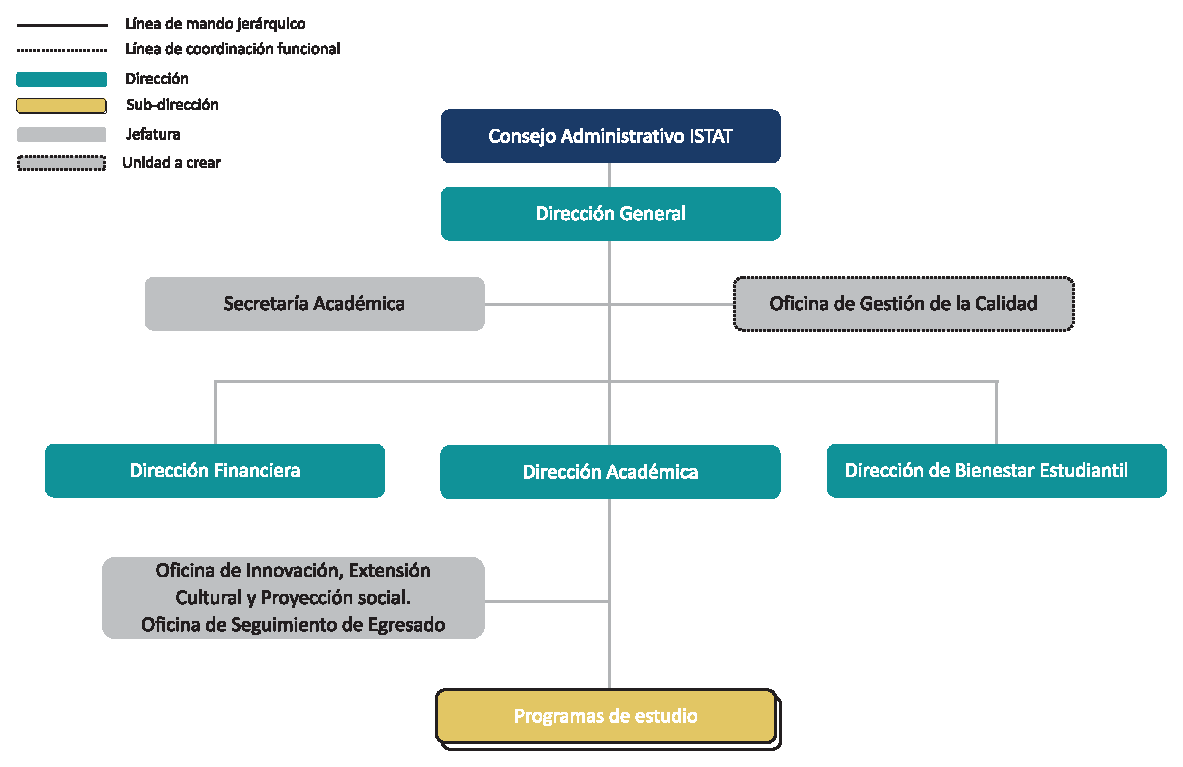
\includegraphics[scale=0.7]{imagenes/organigrama-istat.eps}
	\caption{Organigrama}
	\label{fig:mesh1}
\end{figure}
\subsection{Artículo \arabic{ns}. Consejo Administrativo}
\addtocounter{ns}{1}
El Consejo Administrativo es el órgano de gobierno, gestión, dirección y ejecución académica y administrativa del ISTAT.
\subsection{Artículo \arabic{ns}. Integrantes}
\addtocounter{ns}{1}
El Consejo Administrativo está integrado por: 
\begin{enumerate}
\item El Director general (1) 
\item El Director financiero (1) 
\item El Director de bienestar estudiantil (1) 
\item El Director académico (1) 
\item Coordinadores de programa de estudios (2) 
\item Representante de la promotora (1)
\end{enumerate}
El secretario académico del ISTAT asiste a las sesiones con derecho a voz, sin voto.
\subsection{Artículo \arabic{ns}. Periodo}
\addtocounter{ns}{1}
El período de los miembros del Consejo Administrativo es como sigue: 
\begin{enumerate}
\item El Director General, por tiempo indeterminado, mientras dure su nombramiento.
\item El Director Académico, por el período de dos (2) años. 
\item El Director financiero, el Director de bienestar estudiantil, mientras mantengan vigente su designación. 
\item Representante de la Promotora por el tiempo que permanezcan en sus funciones. 
\end{enumerate}
\subsection{Artículo \arabic{ns}. Asesores}
\addtocounter{ns}{1}
Los asesores de Dirección General, Dirección Financiera, Dirección de Bienestar Estudiantil y Dirección Académica asisten al Consejo Administrativo, cuando son requeridos, con voz y sin derecho a voto. 
\subsection{Artículo \arabic{ns}. Atribuciones}
\addtocounter{ns}{1}
El Consejo Administrativo tiene las siguientes atribuciones:
\begin{enumerate}
\item Aprobar el presupuesto general del ISTAT, el plan anual de adquisiciones de bienes y servicios, autorizar los actos y contratos que atañen al ISTAT y resolver todo lo pertinente a su economía, formulado por la Dirección Financiera.
\item Aprobar el proyecto educativo institucional (PEI), reglamento interno (RI), plan anual de trabajo (PAT), manual de perfil de puestos (MPP), manuales de procesos de régimen académico (MAPRO) y otros que se requieran según la normatividad vigente.
\item Aprobar los planes de estudios propuestos por la dirección académica, de conformidad a la normativa vigente.  
\item Realizar evaluaciones periódicas de los documentos de gestión. 
\item Nombrar al director académico, director financiero y director de bienestar estudiantil, a propuesta de la Promotora, otorgándoles y revocando los poderes respectivos.  
\item Nombrar al secretario académico, a propuesta del director general. 
\item Nombrar, contratar, ratificar, promover y remover a los docentes, a propuesta de los respectivos programas de estudio. 
\item Nombrar, contratar, promover y remover al personal administrativo, a propuesta de la respectiva dirección general. 
\item Conferir los títulos profesionales técnicos, aprobados por el programa de estudios según corresponda.  
\item Aprobar las modalidades de ingreso e incorporación al ISTAT, así como el número de vacantes de cada año para el proceso ordinario de admisión, previa propuesta de los programas de estudio, en concordancia con el presupuesto y el proyecto educativo institucional del ISTAT. 
\item Aprobar la carga académica, administrativa y laboral de sus trabajadores. 
\item Aprobar las sanciones disciplinarias que correspondan al personal y estudiantes.  
\item Aprobar convenios con instituciones nacionales y extranjeras, organismos gubernamentales y no gubernamentales nacionales e internacionales u otros sobre investigación básica e innovación tecnológica, así como otros asuntos relacionados con las actividades del ISTAT. 
\item Cumplir y hacer cumplir los acuerdos de los órganos de dirección, administración y gobierno del ISTAT. 
\item Organizar y dirigir los diversos planes, programas, proyectos y actividades académicas del ISTAT. 
\item Aprobar las directivas académicas y administrativas, emitidas por los órganos académicos y financieros sobre asuntos administrativos o procesos académicos. 
\item Declarar de manera excepcional el receso temporal al ISTAT o cualquiera de sus programas de estudio, cuando las circunstancias lo requieran y lo ameriten, con cargo a dar cuenta al Consejo Administrativo. 
\item Otras especificadas por el presente Reglamento. 
\item Otras no especificadas por el presente Reglamento y que, por la naturaleza de su gestión, le correspondan o le sean determinadas en una directiva.  
\end{enumerate}
\subsection{Artículo \arabic{ns}. Convocatoria}
\addtocounter{ns}{1}
El Consejo Administrativo es convocado por el Director General, mediante esquela, notificada con no menos de siete días hábiles de anticipación a la celebración de la misma, indicando fecha, hora, lugar y asuntos a tratar. No se requiere constancia de recepción de citación.  
\subsection{Artículo \arabic{ns}. Libro de actas}
\addtocounter{ns}{1}
En un libro de actas, debidamente legalizado, se registran todos los acuerdos que adopte el Consejo Administrativo. El acta siempre es aprobada en la misma sesión y firmada por el director general y el secretario académico. Los acuerdos tienen aplicación desde su aprobación.
\section{CAPÍTULO \Roman{re}. DEL DIRECTOR GENERAL}
\addtocounter{re}{1}
\subsection{Artículo \arabic{ns}. Director General: Periodo y requisito.}
\addtocounter{ns}{1}
El Director General es nombrado por la promotora con no menos de cinco (5) años de experiencia y debe cumplir con el requisito establecido por la ley o reglamento vigente.
\subsection{Artículo \arabic{ns}. Director General: Atribuciones en el ámbito educativo}
\addtocounter{ns}{1}
La dirección de la actividad académica por el director general involucra, comprende y abarca: 
\begin{enumerate}
\item Analizar los resultados de las actividades curriculares y emitir lineamientos, instrucciones o directivas a las instancias del ISTAT. 
\item Convocar a los responsables de dirección académica, coordinaciones de los programas de estudio para recibir informes verbales o informaciones generales o específicas sobre la implementación o desarrollo de las actividades académicas, los resultados del aprendizaje y de la gestión curricular. 
\item Emitir opinión sobre aspectos o alcances del desarrollo académico del ISTAT. 
\item Formular directivas, instrucciones o pautas sobre determinados elementos o componentes del quehacer educativo de las áreas académicas y de apoyo. 
\item Formular lineamientos curriculares, pedagógicos, filosófico educativos, administrativos o de gestión académica. 
\item Proponer o conducir comisiones ad hoc o especiales para el desarrollo o implementación de determinado programa de gestión o de calidad u otro para la mejora continua. 
\item Ser informado del desarrollo o funcionamiento de los programas de estudio y de apoyo. 
\item Otras que la naturaleza de la gestión académica institucional exija o tenga necesidad el ISTAT. 
\end{enumerate}
\subsection{Artículo \arabic{ns}. Director General: Atribuciones directorales en el ámbito administrativo, económico y financiero}
\addtocounter{ns}{1}
El director general al dirigir la actividad administrativa, económica y financiera del ISTAT, comprende: 
\begin{enumerate}
\item Asistir como miembro ad hoc a las sesiones, reuniones o similares sobre la gestión administrativa, económica y financiera del ISTAT. 
\item Convocar a los responsables de áreas, oficinas o secciones para informar, entregar o compartir información, datos o resultados de la gestión o los procesos financieros en general. 
\item Ejercer como instancia máxima la revisión de la cuentas, actas, hechos o situaciones generales o específicas de la gestión financiera y económica 
\item Formular lineamientos e instrucciones sobre la gestión administrativa de las áreas académicas y de apoyo. 
\item Impulsar la gestión por procesos en las áreas académicas, administrativas y de apoyo. 
\item Monitorear la gestión administrativa de las áreas académicas y de apoyo, la gestión económica de los programas, proyectos, actividades y acciones del ámbito académico y los resultados financieros. 
\item Presidir y convocar comisiones, comités o equipos técnicos o ad hoc en sesiones plenarias, informáticas o de trabajo sobre la salud financiera del ISTAT. 
\item Observar las alteraciones o prácticas presupuestarias o financieras o administrativas no adecuadas o que afectan a la institución o a las personas. 
\item Recabar informes, resultados o reportes sobre determinados programas, proyectos, actividades o acciones de interés institucional o cuyos resultados afectan, ponen en riesgo, la vida estudiantil, a los miembros de su comunidad o los intereses del ISTAT. 
\item Socializar en la comunidad estudiantil el estado de salud financiera, económica, del ISTAT. 
\item Otras que la naturaleza de la gestión institucional exija o tenga necesidad el ISTAT. 
\end{enumerate}
\subsection{Artículo \arabic{ns}. Director General: Forma de acreditar el grado}
\addtocounter{ns}{1}
En la elección de director general o director académico y otras instancias del ISTAT, el grado de doctor o el de maestría, cuando corresponda al cargo, se acredita con:  
\begin{enumerate}
\item El diploma conferido o revalidado e inscrito en el Registro Nacional de Grados y Títulos de la Superintendencia Nacional de Educación Superior Universitaria (SUNEDU); o,  
\item La constancia emitida por la Superintendencia Nacional de Educación Superior Universitaria (SUNEDU) de que el grado está inscrito en el Registro Nacional de Grados y Títulos, cuando ha sido conferido por otra universidad del país. Y si el grado es de una universidad extranjera, éste de estar previamente reconocido por la SUNEDU e inscrito en el registro antes mencionado, en concordancia de los convenios de reciprocidad cultural y tratados de libre comercio. correspondiente. 
\end{enumerate}
\subsection{Artículo \arabic{ns}. Director General: Tipos de representación}
\addtocounter{ns}{1}
La representación del director general puede ser de dos tipos: 
\begin{enumerate}
\item Representación protocolar. 
\item Representación legal o delegación. 
\end{enumerate}
\subsection{Artículo \arabic{ns}. Director General: Causas y representantes protocolares del Director General}
\addtocounter{ns}{1}
La representación protocolar del Director General, cuando éste por su agenda y responsabilidad no pueda acudir o este impedido, a eventos, actos, sesiones solemnes, reconocimientos, distinciones honorificas o graduaciones o titulaciones; ante entidades públicas o privadas, puede delegar, ser reemplazado, sustituido o representado protocolarmente consecutivamente a decisión el mismo director general, por:  
\begin{enumerate}
\item El director académico.   
\item El director financiero. 
\item El director de bienestar estudiantil. 
\item El secretario académico. 
\end{enumerate}
\subsection{Artículo \arabic{ns}. Director General: Requisitos para ser apoderado legal del ISTAT}
\addtocounter{ns}{1}
Para ser apoderado legal por delegación de poder general o especial, el funcionario o trabajador del ISTAT debe: 
\begin{enumerate}
\item Ser un funcionario o trabajador identificado con el ISTAT, profesional eficiente y moral y éticamente intachable. 
\item Tener la credencial misionera o ministerial. 
\item Tener una función o responsabilidad acorde con las Facultades delegadas. 
\item Experiencia profesional o afín o conocimiento o desempeño en las áreas de los programas de estudio delegadas. 
\end{enumerate}
\subsection{Artículo \arabic{ns}. Director General: Causas y autorización de ausencia temporal del Director General}
\addtocounter{ns}{1}
La ausencia del director general por causas temporales tales como enfermedad aguda, vacaciones, viajes de representación o impedimento físico o fuerza mayor no mayor a un (1) mes o treinta (30) días calendarios, es debidamente autorizada por el Consejo Administrativo, previa solicitud expresa y motivada del director general. 

Las ausencias solo pueden autorizarse por el máximo de tiempo previsto por la promotora. 
\subsection{Artículo \arabic{ns}. Director General: Autorización de ausencia del Director General}
\addtocounter{ns}{1}
La ausencia del Director General por un tiempo superior a un (1) mes o treinta (30) días calendarios, debidos a enfermedad crónica o impedimento físico permanente o fuerza mayor, que le imposibilita asumir o acudir físicamente en su despacho, es autorizada por el Consejo Administrativo del ISTAT, que es convocada por el director académico para una sesión extraordinaria, bajo responsabilidad funcional. 
\subsection{Artículo \arabic{ns}. Director General: Caso de ausencia mayor a dos meses del Director General}
\addtocounter{ns}{1}
Si la ausencia del director general es debido a enfermedad crónica que por su tratamiento o atención médica le requiere un descanso médico o inhabilitación temporal superior a dos (2) meses o sesenta (60) días calendarios la promotora podrá optar por: 
\begin{enumerate}
\item Autorizar la ausencia del titular hasta por el tiempo máximo de ausencia conforme el Estatuto de la promotora; o, 
\item Declarar la remoción del titular y declarar la vacancia del cargo de director general; o, 
\item Solicitar la renuncia del titular. 
\end{enumerate}
La promotora convoca en forma extraordinaria al consejo administrativo y sus acuerdos son adoptados por la mayoría simple.  
\subsection{Artículo \arabic{ns}. Director General: Inexistencia de autorización de ausencia y consecuencias}
\addtocounter{ns}{1}
La inexistencia de autorización motivada para la ausencia del Director General, aprobada por el Consejo Administrativo, es causal automática de remoción por la causal de abandono de cargo y declaración de vacancia por incumplimiento del Estatuto de la promotora y el Reglamento Interno del ISTAT, bajo responsabilidad de quien hace las veces de director general encargado o del director académico. 
\subsection{Artículo \arabic{ns}. Director General: Cómputo del período en caso de vacancia de la autoridad estudiantil}
\addtocounter{ns}{1}
Cuando se declara la vacancia del cargo de Director General por cualquiera de las causales previstas en el Estatuto de la promotora, y el Director General saliente no completo el período, el nuevo director general es elegido para completar el período del director general saliente. 
\subsection{Artículo \arabic{ns}. Director General: Características de la carta de renuncia del Director General}
\addtocounter{ns}{1}
En el caso de renuncia del Director General por medio escrito bajo la modalidad de carta debe reunir obligatoriamente las siguientes características: 
\begin{enumerate}
\item La carta de renuncia puede o no expresar la razón o motivación.  
\item La renuncia al cargo puede ser o no ser irrevocable.  
\item La renuncia debe señalar en forma cierta la fecha en que se dejará la función. 
\item La carta de renuncia puede ser presentada a través de medios físicos o electrónicos, en este último caso a condición de que se dé certeza de la identidad del renunciante y acuse de recibo o entrega.  
\item La carta de renuncia se dirige al órgano que le eligió o a quien lo representa. Estas características se aplican asimismo a las autoridades institucionales de: director académico, director financiero, director de bienestar estudiantil, y otros que por su naturaleza sean necesarios por su función o responsabilidad. 
\end{enumerate}
\subsection{Artículo \arabic{ns}. Autoridad institucional: Disposición y comunicación de la carta de renuncia}
\addtocounter{ns}{1}
En su caso, la carta de renuncia de las autoridades institucionales, es puesta a disposición y/o comunicada por: 
\begin{enumerate}
\item El encargado o responsable del órgano de gobierno, en la sesión a consideración del pleno de miembros. 
\item El encargado o responsable en conocimiento de la Promotora del ISTAT. 
\item El secretario general en conocimiento de las entidades de educación u otras que corresponda.  
\end{enumerate}

\section{CAPÍTULO \Roman{re}. DEL DIRECTOR ACADÉMICO}
\addtocounter{re}{1}
\subsection{Artículo \arabic{ns}. Director Académico: Periodo}
\addtocounter{ns}{1}
El Director académico es elegido por el Consejo Administrativo, por el período de dos (2) años y puede ser reelegido.
\subsection{Artículo \arabic{ns}. Atribuciones del Director académico en la gestión académica}
\addtocounter{ns}{1}
Las atribuciones del Director académico en la gestión académica de los programas de estudios del ISTAT comprenden: 
\begin{enumerate}
\item Acompañar el desarrollo de las actividades académicas en cada período. 
\item Apoyar y empoderar a las autoridades académicas dependientes funcionalmente de su despacho. 
\item Cautelar la observancia de los principios de la filosofía educativa adventista en la planificación, desarrollo y evaluación de los programas de estudio, su implementación, desarrollo y evaluación curricular, bajo responsabilidad funcional. 
\item Conformar, convocar y dirigir grupos de trabajo, subcomisiones, reuniones, talleres y otros para el cumplimiento de sus funciones. 
\item Comunicar las contingencias, riesgos y problemáticas de las dependencias a su cargo, previa la intervención en caso de emergencias. 
\item Constituir comités y/o comisiones sobre asuntos, materias académicas o de formación, aprendizaje y otros para fortalecer la gestión o los propósitos educacionales. 
\item Cumplir y hacer cumplir los lineamientos pedagógicos, didácticos, de la integración fe-enseñanza en el proceso de formación profesional de los programas de estudios. 
\item Dirigir, monitorear y supervisar la formulación del plan de vida docente, su desarrollo y evaluar los resultados en cada período académico. 
\item Formular, sustentar y desarrollar programas, proyectos, actividades y acciones conducentes a la mejora continua y presentarlos ante las instancias respectivas. 
\item Formular, presentar y ejecutar programas de capacitación pedagógica, educativa, curricular y otras para fortalecer las capacidades docentes. 
\item Formular, presentar, sustentar, implementar y evaluar los cronogramas académicos institucionales y socializar en la comunidad educativa. 
\item Formular, presentar, sustentar e implementar programas de incentivos y motivación docente y del personal de apoyo académico de los programas de estudio. 
\item Garantizar el funcionamiento normal del proceso de enseñanza-aprendizaje, las sesiones de clase, los aspectos logísticos y la asignación, aplicación y disposición de los recursos. 
\item Inventariar los vacíos, deficiencias y desafíos del proceso de enseñanza aprendizaje de los programas de estudio y canalizar, formular o implementar las soluciones más inmediatas.   
\item Monitorear el programa, proyectos, actividades y acciones para la capacitación pedagógica docente en cada período académico y delinear su reformulación y aplicación. 
\item Monitorear el cumplimiento de los cronogramas académicos de matrícula de la institución. 
\item Observar y hacer cumplir las políticas, lineamientos e instrucciones emanadas del director general. 
\item Organizar y fortalecer el funcionamiento de las direcciones y oficinas de las áreas bajo su dependencia. 
\item Participar de la mejora continua de los procesos, procedimientos y subprocedimientos del sistema de gestión de la calidad.  
\item Solicitar informes, reportes, memorias y otros a los programas de estudio sobre la gestión académica u otros específicos. 
\item Sustentar ante otras instancias y órganos de gobierno la propuesta de programas de estudios, previa elaboración de los proyectos respectivos. 
\item Otras que la naturaleza de la gestión académica. 
\end{enumerate}
\subsection{Artículo \arabic{ns}. Director académico: Atribuciones del director académico en el ámbito curricular}
\addtocounter{ns}{1}
El director académico en la formulación, aprobación, implementación y evaluación curricular del diseño curricular o currículo y de sus componentes, tiene las atribuciones siguientes: 
\begin{enumerate}
\item Acompañar la formulación del proyecto de diseño curricular o currículo institucional y de los programas de estudio. 
\item Articular la formulación del proyecto de diseño curricular o currículo con la participación de las unidades académicas de la institución. 
\item Apoyar a las direcciones u oficinas responsables de la formulación, implementación y evaluación del diseño curricular, currículo y sus componentes. 
\item Asistir a los equipos, comités de diseño y evaluación curricular de los recursos, logística y soportes que permitan la consecución de los propósitos. 
\item Formular, implementar y evaluar lineamientos, políticas, directrices o manuales a través de sus dependencias, comités o responsables bajo su dependencia. 
\item Impulsar la evaluación curricular en forma sistemática, regular y controlada en los programas de estudio. 
\item Impulsar la capacitación, formación, del docente en áreas de diseño y evaluación curricular. 
\item Informar a dirección general sobre las actividades y acciones sobre diseño y evaluación curricular.  
\item Monitorear las actividades y acciones formuladas, implementadas y ejecutadas por las direcciones, oficinas y responsables de diseño y evaluación curricular. 
\item Participar y socializar los resultados de la evaluación de los currículos o modelos curriculares o planes de estudios de los programas de estudio. 
\item Presentar los planes de mejora del diseño o currículo y sus componentes, definidos por los programas de estudio, comités respectivos. 
\item Socializar en los equipos técnicos, los programas de estudio y la comunidad educativa los resultados de la evaluación curricular, de sus componentes: perfil de ingreso, perfil de egreso, perfil profesional, plan de estudios, malla curricular, sistema de evaluación y otros.  
\item Racionalizar los recursos en la gestión curricular que fortalezcan el desempeño académico de los programas de estudio. 
\item Otras que la planificación, implementación y ejecución del diseño curricular requieren. 
\end{enumerate}
\subsection{Artículo \arabic{ns}. Director académico: Ausencia temporal}
\addtocounter{ns}{1}
La ausencia director académico por causas temporales tales como enfermedad aguda o crónica, vacaciones, viajes de representación o impedimento físico o fuerza mayor, es debidamente autorizada por el Consejo Administrativo, previa solicitud expresa y motivada del director académico. 

Las ausencias solo pueden autorizarse por el máximo de tiempo previsto en el consejo administrativo y se regulan en la misma amplitud y presupuestos que los establecidos para el director general. 
\subsection{Artículo \arabic{ns}. Director académico: Inexistencia de autorización de ausencia y consecuencias}
\addtocounter{ns}{1}
La inexistencia de autorización motivada para la ausencia del director académico, es causal de remoción automática y declaración de vacancia por incumplimiento del Reglamento Interno del ISTAT. 

Todo lo previsto y presupuestado para el cargo del director general es también de aplicación para el cargo de director académico. 
\subsection{Artículo \arabic{ns}. Director académico: Representación protocolar}
\addtocounter{ns}{1}
La representación protocolar del director académico, cuando éste por su agenda y responsabilidad no pueda acudir o este impedido de asistir, a eventos o actos o sesiones o ceremonias protocolares o académicas, tales como sesiones solemnes, reconocimientos o distinciones honorificas o graduaciones; ante entidades públicas o privadas, puede delegar, ser reemplazado o sustituido o representado protocolarmente por:  
\begin{enumerate}
\item El docente con la categoría máxima o con mayor antigüedad en la docencia en el ISTAT, para el caso del director académico. 
\end{enumerate}
\section{CAPÍTULO \Roman{re}. DEL DIRECTOR FINANCIERO}
\addtocounter{re}{1}
\subsection{Artículo \arabic{ns}. Director Financiero: Periodo}
\addtocounter{ns}{1}
El Director financiero es elegido por el Consejo Administrativo, por el período de dos (2) años y puede ser reelegido.
\subsection{Artículo \arabic{ns}. Director financiero: Atribuciones en el ámbito económico}
\addtocounter{ns}{1}
Son funciones del director financiero, las siguientes: 
\begin{enumerate}
\item Acompañar la gestión económica de los programas de estudio, de apoyo, áreas y demás unidades del ISTAT. 
\item Cautelar, monitorear, la recaudación de los ingresos resultado de las actividades educativas del ISTAT. 
\item Coordinar con las instancias u órganos de auditoría sobre los riesgos, debilidades en la gestión económica del ISTAT. 
\item Dirigir preventivamente las estrategias de recaudación de los ingresos en el período académico.  
\item Dictar los lineamientos, políticas y directivas sobre la aplicación de medidas preventivas, de seguridad interna y externa para la recaudación de los ingresos y egresos. 
\item Determinar los lineamientos, políticas y directivas sobre el gasto operacional del ISTAT. 
\item Emprender programas, proyectos, planes, actividades y acciones para la captación de recursos económicos. 
\item Formular políticas, directivas para la captación de donaciones, legados, subvenciones u otros. 
\item Formular, presentar y proponer las medidas de racionalización económica en los gastos operacionales del ISTAT. 
\item Monitorear el desempeño y las decisiones económicas de los responsables Organizar equipos técnicos, multidisciplinarios, especiales para abordar temáticas, situaciones o circunstancias de contexto o gestión general de los recursos económicos del ISTAT. 
\item Reportar, socializar, informar del estado, condición y calidad de los estados financieros del ISTAT, sus programas de estudio, de apoyo, áreas y otros en el período académico. 
\item Supervisar la aplicación, cumplimiento, observancia de los lineamientos, políticas y directrices económicas en la gestión del ISTAT. 
\item Otras que el reglamento u otros señalen. 
\end{enumerate}
\subsection{Artículo \arabic{ns}. Director financiero: Atribuciones en el ámbito presupuestario}
\addtocounter{ns}{1}
Son atribuciones del director financiero en el ámbito presupuestario, las siguientes. 
\begin{enumerate}
\item Disponer las medidas de gestión presupuestaria en el ISTAT. 
\item Formular el presupuesto y concertar los mismos con los programas de estudio, de apoyo, áreas. 
\item Formular, presentar y proponer los ajustes a las cuentas, partidas presupuestarias fundados en el estado económico, financiero y de sostenibilidad del ISTAT. 
\item Identificar, pronosticar, las tendencias económicas y financieras del ISTAT que pueden afectar, incidir, favorecer o soporten la salud y sostenibilidad financiera institucional. 
\item Perfilar las fuentes de financiamiento del presupuesto institucional. 
\item Reformular el plan presupuestario y fundamentar sus modificaciones, correcciones ante los órganos de gobierno. 
\item Socializar los lineamientos, políticas, directivas y normas presupuestarias. 
\item Otras que el reglamento u otros señalen. 
\end{enumerate}
\subsection{Artículo \arabic{ns}. Director financiero: Atribuciones en el ámbito financiero}
\addtocounter{ns}{1}
Son atribuciones del director financiero en el ámbito administrativo, las siguientes: 
\begin{enumerate}
\item Analizar el estado, calidad, características económico-financieras del periodo, momento, de manera vertical u horizontal, ratios del ISTAT.  
\item Analizar la rentabilidad de los servicios educativos y su aporte a la sostenibilidad económica del ISTAT. 
\item Analizar el costo del servicio educativo, costos de servicios conexos o derivados, en base a estudios económico-financieros, del mercado o plaza, del sector poblacional y la misión del ISTAT. 
\item Accionar los mecanismos administrativos internos de contingencia en situaciones, casos, hechos o emergencias institucionales no presupuestadas. 
\item Cautelar la generación de valor en cada y todas las actividades académicas, las de apoyo académico y servicios conexos o derivados del ISTAT. 
\item Controlar la estructura de capital, el nivel de endeudamiento, negociación y ejecución de operaciones financieras de mediano y largo plazo en el período académico. 
\item Coordinar la preparación de los presupuestos operativos de las unidades académicas estratégicas del ISTAT. 
\item Definir y monitorear la ejecución de incentivos u ofertas en los servicios educativos para la sostenibilidad financiera. 
\item Elaborar el presupuesto considerando el estado de los ingresos y egresos, el nivel de liquidez y las obligaciones internas y con terceros del ISTAT. 
\item Establecer y monitorear los mecanismos de seguimiento de la calidad del gasto en el ISTAT. 
\item Formular, proponer y mantener actualizada la estructura de los Ingresos y egresos, en coordinación con las otras direcciones administrativas del ISTAT. 
\item Gestionar la operatividad de los soportes tecnológicos presupuestarios con un enfoque de integración intersistémica, en coordinación con las instancias operativas del ISTAT. 
\item Perfilar el presupuesto de inversiones sobre la base de proyectos con todos y cada uno de los componentes técnicos requeridos en el corto mediano y largo plazo. 
\item Promover el perfeccionamiento permanente de la técnica presupuestaria y la mejora de las capacidades y competencias en la gestión presupuestaria. 
\item Proponer oportunidades de negocio educativo o derivados en el mediano y el largo plazo como fuentes de financiamiento alternativo, fundamentados en proyectos compuestos con todos y cada uno de los requerimientos técnicos, sustentados ante los órganos de gobierno. 
\item Recabar opiniones, asesorías técnicas y percepciones sobre los comportamientos del mercado o plaza en el ámbito educativo o los servicios o productos del ISTAT, frente a las similares o de terceros. 
\item Trasmitir con claridad los lineamientos, políticas y directrices de gestión financiera en el período y pronosticar su permanencia o caducidad en el período. 
\item Otras que el reglamento u otros le señalen. 
\end{enumerate}
\subsection{Artículo \arabic{ns}. Director financiero: Atribuciones en el ámbito del talento humano}
\addtocounter{ns}{1}
Son atribuciones del director financiero en el ámbito administrativo, las siguientes: 
\begin{enumerate}
\item Acatar, implementar y supervisar el cumplimiento de las disposiciones o normatividad laboral en las actividades estratégicas y operativas del ISTAT. 
\item Accionar los mecanismos administrativos, financieros y otros para la resolución de problemáticas, requerimientos o necesidades del talento humano conflictivas o contingentes. 
\item Actuar como apoderado ante las instancias prejudiciales, judiciales, arbitrales o conciliatorias nacionales o internacionales por temas de la gestión del talento humano. 
\item Accionar en representación y defensa legal del ISTAT en base a las facultades generales de administración, laborales y judiciales otorgadas o delegadas. 
\item Conducir los procesos de selección, reclutamiento y contratación, cualesquiera sean las modalidades y los regímenes laborales del personal del ISTAT. 
\item Conducir la determinación de las plazas o puestos de trabajos vacantes o requeridos por las actividades y fines del ISTAT. 
\item Consensuar con la administración del ISTAT las políticas, directrices y normas operativas salariales o remunerativas. 
\item Empoderar la gestión del recurso humano a partir de la toma de decisiones descentralizada y contextualizada por el responsable en el ISTAT. 
\item Favorecer la implementación y otorgamiento de incentivos económico o no económico al personal del ISTAT. 
\item Fortalecer la gestión de programas, proyectos, actividades y acciones de clima laboral saludable, óptimo y de calidad 
\item Solicitar informes, reportes, estados o ayudas memorias sobre la gestión de personal en los ámbitos remunerativos, beneficios sociales, tardanzas, permisos o licencias laborales y otras incidencias para la toma de decisiones o disposición de los recursos financieros del ISTAT. 
\item Sustentar las restricciones o límites en el gasto o atención al personal del ISTAT aplicables en el período académico. 
\item Valorar el aporte de los trabajadores en el contexto de sus responsabilidades y rol desempeñado. 
\item Otras que el reglamento u otros señalen.  
\end{enumerate}
\subsection{Artículo \arabic{ns}. Director financiero: Atribuciones en el ámbito de los servicios generales y de apoyo académico}
\addtocounter{ns}{1}
Son atribuciones del director financiero en el ámbito de servicios generales y de apoyo académico, las siguientes: 
\begin{enumerate}
\item Analizar la eficacia y eficiencia de los servicios generales y de apoyo académico en la generación de valor, rentabilidad y sostenibilidad del ISTAT. 
\item Cautelar, monitorear, que los servicios generales y de apoyo académico estén en pleno, perfecto y normal funcionamiento. 
\item Conservar, acrecentar y potenciar la calidad de los servicios generales y de apoyo. 
\item Favorecer la creatividad y el emprendimiento de negocios colaterales a las actividades académicas que posibiliten la comodidad, atención personalizada y calidad en los servicios. 
\item Generar oportunidades, ofertas, de servicios generales y de apoyo estratégicos para los estudiantes y personal del ISTAT. 
\item Proponer los lineamientos, políticas y directrices en la gestión de los servicios generales y de apoyo del ISTAT. 
\item Racionalizar el acceso y uso de los recursos en el funcionamiento de los servicios generales y de apoyo. 
\item Sustituir materiales o insumos por biodegradables que permitan un ambiente e institución saludable y libre de contaminantes en el ISTAT. 
\item Otras que el reglamento u otros señalen. 
\end{enumerate}
\section{CAPÍTULO \Roman{re}. DEL DIRECTOR DE BIENESTAR ESTUDIANTIL}
\setcounter{re}{1}
\subsection{Artículo \arabic{ns}. Director de bienestar estudiantil: Periodo}
\addtocounter{ns}{1}
El Director de bienestar estudiantil es elegido por el Consejo Administrativo, por el período de dos (2) años y puede ser reelegido.
\subsection{Artículo \arabic{ns}. Director de bienestar estudiantil: Rol y función esencial}
\addtocounter{ns}{1}
El rol del director de bienestar estudiantil es esencial para el cumplimiento de los propósitos educacionales; es pues el responsable de hacer viable, mantener, fortalecer, priorizar e implementar la atención al estudiante durante su estancia, quehacer y vida estudiantil en el ISTAT.  

Para efectivizar la función del director de bienestar estudiantil hace uso de los medios, recursos y mecanismos a su alcance en el corto, mediano y largo plazo. 
\subsection{Artículo \arabic{ns}. Director de bienestar estudiantil: Atribuciones en el ámbito de los programas de atención al estudiante}
\addtocounter{ns}{1}
Son atribuciones del director de bienestar estudiantil en el ámbito de los programas de atención al estudiante, las siguientes: 
\begin{enumerate}
\item Analizar la eficacia y eficiencia de los programas de atención al estudiante: alimentación, recreación, salud física y emocional, el deporte, cultura y otros que generen de valor: satisfacción, posicionamiento, rentabilidad y sostenibilidad del ISTAT. 
\item Acompañar, a través de los responsables de los programas, al estudiante en la implementación y participación en el período académico. 
\item Atender los requerimientos y necesidades de medios, recursos o soportes en el funcionamiento de los programas y en su caso encaminar estos requerimientos antes las instancias internas respectivas. 
\item Cautelar, monitorear, que los programas de atención al estudiante estén activados, en desarrollo y normal estado de acceso.  
\item Coordinar con las áreas o departamentos o responsables correspondientes el uso de recursos, medios y soportes logísticos materiales o inmateriales para el funcionamiento, prestación de los servicios al estudiante. 
\item Conservar, acrecentar y potenciar la calidad de los programas de atención al estudiante en el período académico. 
\item miento de los programas de atención al estudiante, docente y personal del ISTAT. 
\item Cuidar que en el desarrollo de los programas de atención al estudiante se observe, preserve, cautele el cumplimiento del marco axiológico, filosófico, la cultura organizacional y clima institucional del ISTAT. 
\item Fortalecer el desarrollo e implementación de los programas como complemento de la actividad académica que posibiliten la comodidad, atención personalizada y calidad en sus actividades y acciones.  
\item Formular, presentar y proponer la aprobación de los programas de atención al estudiante ante el órgano de gobierno en el período académico. 
\item Garantizar la implementación de medidas, medios, recursos, logística de soporte disponibles para la ejecución y puesta en marcha de los programas de atención al estudiante. 
\item Generar ofertas, nuevas modalidades o programas complementarios para los estudiantes y personal del ISTAT. 
\item Gestionar los recursos de financiamiento de los programas con eficiencia y sostenibilidad en el período presupuestario del ISTAT. 
\item Instruir a los responsables y operadores de los programas de atención al estudiante las instrucciones sobre cuidado, observar el respeto, preservar la intimidad e integridad moral y física de los estudiantes. 
\item Proponer los lineamientos, políticas y directrices en la gestión de los programas de atención al estudiante del ISTAT. 
\item Racionalizar el acceso y uso de los recursos en el funcionamiento de los programas de atención al estudiante. 
\item Sustituir recursos, materiales o insumos por biodegradables en los programas, preservando el ambiente e institución saludable y libre de contaminantes en el ISTAT. 
\item Otras que el reglamento u otros señalen. 
\end{enumerate}
\subsection{Artículo \arabic{ns}. Director de bienestar estudiantil: Atribuciones en el ámbito del desarrollo espiritual}
\addtocounter{ns}{1}
Son atribuciones del director de bienestar estudiantil en el ámbito del desarrollo espiritual, las siguientes: 
\begin{enumerate}
\item Analizar la eficacia y eficiencia de los programas de atención al estudiante: alimentación, recreación, salud física y emocional, el deporte, cultura y otros que generen de valor: satisfacción, posicionamiento, rentabilidad y sostenibilidad del ISTAT. 
\item Acompañar, a través de los responsables de los programas, al estudiante en la implementación y participación en el período académico. 
\item Atender los requerimientos y necesidades de medios, recursos o soportes en el funcionamiento de los programas y en su caso encaminar estos requerimientos antes las instancias internas respectivas. 
\item Cautelar, monitorear, que los programas de atención al estudiante estén activados, en desarrollo y normal estado de acceso.  
\item Coordinar con las áreas o departamentos o responsables correspondientes el uso de recursos, medios y soportes logísticos materiales o inmateriales para el funcionamiento, prestación de los servicios al estudiante. 
\item Conservar, acrecentar y potenciar la calidad de los programas de atención al estudiante en el período académico. 
\item Comunicar, difundir, en la comunidad educativa la puesta en marcha, la oferta, el funcionamiento de los programas de atención al estudiante, docente y personal del ISTAT. 
\item Cuidar que en el desarrollo de los programas de atención al estudiante se observe, preserve, cautele el cumplimiento del marco axiológico, filosófico, la cultura organizacional y clima institucional del ISTAT. 
\item Fortalecer el desarrollo e implementación de los programas como complemento de la actividad académica que posibiliten la comodidad, atención personalizada y calidad en sus actividades y acciones.  
\item Formular, presentar y proponer la aprobación de los programas de atención al estudiante ante el órgano de gobierno en el período académico. 
\item Garantizar la implementación de medidas, medios, recursos, logística de soporte disponibles para la ejecución y puesta en marcha de los programas de atención al estudiante. 
\item Generar ofertas, nuevas modalidades o programas complementarios para los estudiantes y personal del ISTAT. 
\item Gestionar los recursos de financiamiento de los programas con eficiencia y sostenibilidad en el período presupuestario del ISTAT. 
\item Instruir a los responsables y operadores de los programas de atención al estudiante las instrucciones sobre cuidado, observar el respeto, preservar la intimidad e integridad moral y física de los estudiantes. 
\item Proponer los lineamientos, políticas y directrices en la gestión de los programas de atención al estudiante del ISTAT. 
\item Racionalizar el acceso y uso de los recursos en el funcionamiento de los programas de atención al estudiante. 
\item Sustituir recursos, materiales o insumos por biodegradables en los programas, preservando el ambiente e institución saludable y libre de contaminantes en el ISTAT. 
\item Otras que el reglamento u otros señalen. 
\end{enumerate}
\subsection{Artículo \arabic{ns}. Director de bienestar estudiantil: Atribuciones en el ámbito del desarrollo espiritual}
\addtocounter{ns}{1}
Son atribuciones del director de bienestar estudiantil en el ámbito del desarrollo espiritual, las siguientes: 
\begin{enumerate}

\item Ajustar los programas, actividades y acciones de desarrollo espiritual en la implementación en la comunidad educativa del ISTAT. 
\item Analizar la eficacia y eficiencia de los programas de desarrollo espiritual en el ISTAT, valorando la generación de un ambiente espiritual, de comunión, comunidad de fe y que generen valor en la comunidad educativa: satisfacción, posicionamiento y sostenibilidad axiológica y filosófica, identidad y cultura organizacional en el ISTAT. 
\item Aplicar los lineamientos, directrices del desarrollo espiritual formulados por la Promotora del ISTAT. 
\item Articular los esfuerzos a través de programas, proyectos, planes, actividades y acciones de desarrollo espiritual en el ISTAT, con el carácter de únicos, unitarios, orgánicos e institucionales. 
\item Atender los requerimientos y necesidades de medios, recursos o soportes en el funcionamiento de los servicios de apoyo al estudiante y en su caso encaminar estos requerimientos antes las instancias internas respectivas. 
\item Cautelar, monitorear, que los servicios de atención al estudiante estén activados, en desarrollo y normal estado de acceso.  
\item Coordinar con la dirección de bienestar estudiantil, los lineamientos, políticas y estrategias de desarrollo espiritual para la comunidad educativa.
\item Coordinar con	las áreas o responsables correspondientes el uso de recursos, medios y soportes logísticos materiales o inmateriales para el desarrollo e implementación de programas, proyectos, actividades y acciones de desarrollo espiritual. 
\item Comunicar, difundir, en la comunidad educativa la cultura del desarrollo espiritual, sus símbolos, slogans, referentes y todo elemento comunicacional en todos los escenarios provistos en el ISTAT. 
\item Concordar con los operadores de los programas, proyectos, planes, actividades y acciones del desarrollo espiritual, los alcances, el ámbito y extensión de su ejecución o implementación en el quehacer y la vida estudiantil. 
\item Cuidar en el desarrollo espiritual el cumplimiento, observancia, del marco axiológico, filosófico, la cultura organizacional y clima espiritual cristiano del ISTAT. 
\item Determinar el cronograma del desarrollo espiritual  a nivel institucional, identificando los programas, proyectos, planes y actividades en forma anual, semestral, mensual y semanal. 
\item Fortalecer el desarrollo espiritual en cualquiera de las actividades del ISTAT sean de carácter académica, educativa, recreativa, deportiva, social o cultural, que afiancen la comunidad de fe, el ambiente cristiano.   
\item Formular, presentar y proponer la aprobación de los programas, planes, proyectos, actividades y acciones de desarrollo espiritual ante el órgano de gobierno respectivo en el período académico. 
\item Garantizar la implementación de medidas, medios, recursos, logística de soporte disponibles para la ejecución y puesta en marcha de los programas, planes, proyectos, actividades y acciones de desarrollo espiritual. 
\item Generar y mantener nuevas modalidades de desarrollo espiritual disponibles para la comunidad educativa del ISTAT. 
\item Gestionar los recursos de financiamiento del desarrollo espiritual con eficiencia y sostenibilidad en el período presupuestario del ISTAT. 
\item Organizar eventos de capacitación, entrenamiento, para los operadores del desarrollo espiritual y los responsables de los programas de estudio, de apoyo y otras del ISTAT. 
\item Perfilar los lineamientos, estrategias, directrices de aplicación en las unidades académicas y operarlas a partir de las direcciones de bienestar estudiantil. 
\item Promover y monitorear el desarrollo espiritual. 
\item Proponer los lineamientos, políticas y directrices institucionales, aplicables, de observancia obligatoria en la gestión del desarrollo espiritual del ISTAT. 
\item Otras que el reglamento u otros señalen. 
\end{enumerate}
\subsection{Artículo \arabic{ns}. Director de bienestar estudiantil: Atribuciones en el ámbito de la disciplina y conducta estudiantil}
\addtocounter{ns}{1}
Son atribuciones del director de bienestar estudiantil en el ámbito de la disciplina y conducta estudiantil, las siguientes: 
\begin{enumerate}
\item Activar los mecanismos, medios y recursos dispuestos por los reglamentos y procedimientos para cautelar la protección de la integridad de los miembros de la comunidad educativa. 
\item Atender las inquietudes sobre el régimen disciplinario del ISTAT a través de sus unidades operativas adscritas. 
\item Cautelar la intimidad, honor y buen nombre de los estudiantes y docentes en los procesos preliminares disciplinarios, cautelando los derechos y preservando las declaraciones, pruebas u otras. 
\item Coordinar con los programas de estudio y de apoyo las medidas preventivas, de innovación y proceso disciplinario sobre estudiantes. 
\item Cumplir el rol dispuesto en las normas de conducta respecto de informar, presentar, los elementos, indicios, pruebas testimoniales u otras que permitan dilucidar, tener certeza, para iniciar proceso disciplinario a estudiantes, docentes o personal del ISTAT. 
\item Difundir sistemática y masivamente a la comunidad educativa los alcances, contenido y consecuencias de las inconductas o comportamientos que lesionan el marco disciplinario del ISTAT. 
\item Disponer, previa evaluación de la comisión interna, el inicio de proceso disciplinario a estudiantes o docentes, remitiendo el informe respectivo a la comisión de disciplina respectiva. 
\item Emitir los informes, reportes, estado o ayuda memoria derivados de la investigación preliminar o procesos disciplinarios. 
\item Notificar al estudiante o docente los resultados de la evaluación preliminar sobre los hechos materia del proceso disciplinario. 
\item Participar a través de las direcciones de bienestar estudiantil de los programas de estudio en los procesos disciplinarios, el marco conductual de la comunidad educativa. 
\item Proponer las medidas, medios y mecanismos preventivos para un ambiente de observancia y cumplimiento de las normas de conducta del ISTAT. 
\item Recibir denuncias o quejas sobre inconductas, comportamientos o actos ilícitos que vulneran el orden disciplinario del ISTAT.   
\item Otras que el presente reglamento u otros señalen 
\end{enumerate}
%--------------------------------------------------------------------------------
\part{TÍTULO \Roman{par}. DE LA ORGANIZACIÓN ACADÉMICA}
\addtocounter{ns}{1}
\section{CAPÍTULO \Roman{re}. DE LOS PROGRAMAS DE ESTUDIO}
\addtocounter{re}{1}
\subsection{Artículo \arabic{ns}. Naturaleza del programa de estudios}
\addtocounter{ns}{1}
El programa de estudio por su naturaleza y carácter, se estructura como un órgano: 
\begin{enumerate}
\item ÚNICA: El programa de estudio es única, no existe otro que lo reemplace o sustituya. 
\item INSTITUCIONAL: Programa de estudio en su funcionamiento, cobertura o competencia es de carácter institucional. 
\item DESCENTRALIZADA: La estructura organizacional del programa de estudio se extiende en sus funciones y funcionamiento a través de niveles de responsabilidad en la dirección y coordinación de sus fines y propósitos. 
\end{enumerate}
\subsection{Artículo \arabic{ns}. Programa de estudio: Aprobación de la estructura organizacional y funcional}
\addtocounter{ns}{1}
El ISTAT en forma corporativa estructura y aprueba por Consejo Administrativo los niveles organizacionales, niveles y los responsables funcionales de los programas de estudio respetando su naturaleza y campo profesional, previa propuesta concertada de la dirección general y con los coordinadores de los mismos programas. 

En dicho diseño organizacional corporativo se considera al mismo programa de estudios ubicados en la institución. 
\subsection{Artículo \arabic{ns}. Programa de estudio: Creación, fusión, reorganización o escisión}
\addtocounter{ns}{1}
La creación, fusión, escisión, supresión o reorganización orgánica o funcional de un programa de estudios se sustenta en un proyecto fundamentado que debe contener como mínimo: 
\begin{enumerate}
\item Fundamentación. 
\item Justificación. 
\item Académica. 
\item Administrativa. 
\item Estructura, Modelo Organizacional y Funcional. 
\item Prospectiva de desarrollo 
\item Costo financiero. 
\item Anexos 
\end{enumerate}
\subsection{Artículo \arabic{ns}. Programa de estudios: Comisión Ad hoc para creación, fusión, escisión, reorganización}
\addtocounter{ns}{1}
El proyecto de creación, fusión, escisión, supresión o reorganización de un programa de estudios es formulado por una comisión ad hoc y con la participación de su promotora. Es propuesta por el director general al Consejo Administrativo para su aprobación y derivado a la promotora para su ratificación. 
\subsection{Artículo \arabic{ns}. Programa de estudios: Adscripción de programas de estudios}
\addtocounter{ns}{1}
El programa de estudios puede tener uno o más planes de estudio, es decir desarrollar uno o más diseño curriculares o currículos, bajo la condición que éstos correspondan al área de conocimientos profesionales afines o vinculados. 
\subsection{Artículo \arabic{ns}. Programas de estudio del ISTAT}
\addtocounter{ns}{1}
Los programas de estudio del ISTAT son las siguientes: 
\begin{enumerate}
\item Desarrollo de Sistemas de Información
\item Enfermería Técnica
\end{enumerate}
\subsection{Artículo \arabic{ns}. Programa de formación continua: Concepción y alcances}
\addtocounter{ns}{1}
El ISTAT gestiona los programas de formación continua a distancia cuyo fundamento pedagógico involucra el uso de tecnologías, técnicas andragógicas o educación en entornos virtuales.
\subsection{Artículo \arabic{ns}. Programa de formación continua: Operador de la gestión académica y administrativa}
\addtocounter{ns}{1}
El ISTAT gestiona los programas de educación a distancia a través de dos niveles:
\begin{enumerate}
\item Nivel de programa de estudios: En el aspecto académico, el proceso enseñanza aprendizaje, las estrategias de aprendizaje y evaluación del aprendizaje, la didáctica y el desempeño pedagógico del docente o tutor o personal de apoyo, el sistema de evaluación y los resultados o rendimiento académico, y todo aquello que significa el desarrollo de la planificación del programa de formación continua bajo la modalidad. 
\item Nivel de Coordinación a distancia del programa de formación continua. Es una unidad académico-administrativa especializada en la gestión académico-administrativa de la modalidad de estudios que planifica, organiza, desarrolla y evalúa el funcionamiento, sostenibilidad, del servicio educativo haciendo uso de los medios y recursos dispuestos por el ISTAT. Está a cargo de un coordinador nombrado por el Consejo Administrativo a propuesta del coordinador del programa de estudio.
\end{enumerate}
\subsection{Artículo \arabic{ns}. Programa de formación continua: Propósitos y finalidad}
\addtocounter{ns}{1}
El ISTAT planea, proyecta, desarrolla y evalúa programas de formación continua a distancia con el objetivo de: 
\begin{enumerate}
\item El programa de formación promueve un proceso educativo integral y permanente que se desarrolla a lo largo de la vida y tiene como objetivo adquirir, perfeccionar o actualizar conocimientos, aptitudes, capacidades personales y/o profesionales, en mejora del desempeño laboral. No conlleva a la obtención del grado académico o título.
\item Cumplir la misión del ISTAT, así como el de su Promotora, favoreciendo la igualdad de oportunidades educativas o formativas en la formación continua. 
\item Contextualizar el uso de las tecnologías de la comunicación a procesos de enseñanza-aprendizaje, potenciando su masificación, uso responsable y trascendente. 
\item Desarrollar el entorno virtual como un medio educativo en el cumplimiento de sus fines y propósitos educacionales. 
\item Posicionar el modelo educativo del ISTAT a través de programas de formación continua socialmente pertinentes y sostenibles.
\end{enumerate}
\subsection{Artículo \arabic{ns}. Programa de formación continua: Marco normativo obligatorio}
\addtocounter{ns}{1}
Los programas de formación continua se brindan en las modalidades presencial, semipresencial o a distancia. No deben interferir con el normal desarrollo de los programas de estudios y son regulados por los lineamientos académicos generales. 
\subsection{Artículo \arabic{ns}. Programa de formación continua: Proyecto de diseño curricular}
\addtocounter{ns}{1}
El proyecto del programa de formación continua a distancia es propuesto por las coordinaciones de los programas de estudio y aprobados en el Consejo Administrativo. 
\subsection{Artículo \arabic{ns}. Programa de formación continua: Requisitos específicos de Admisión}
\addtocounter{ns}{1}
Los requisitos de admisión a los programas de formación continua a distancia son específicos a la modalidad de estudios, difieren de los programas presenciales.  

Todos los postulantes rinden una evaluación que permite evaluar sus niveles de conocimientos básicos y acreditar el perfil de ingreso del programa de formación continua respectiva. 
\subsection{Artículo \arabic{ns}. Programa de formación continua: Aplicación del Reglamento de Estudios a la modalidad}
\addtocounter{ns}{1}
La modalidad a distancia en general es normada en su desarrollo académico por el Reglamento de Estudios; sin embargo, en aspectos específicos puede ser regulado por otros reglamentos específicos del ISTAT. 
%--------------------------------------------------------------
\section{SUBCAPÍTULO \Roman{su}. DEL COORDINADOR DEL PROGRAMA DE ESTUDIOS}
\setcounter{re}{1}
\subsection{Artículo \arabic{ns}. Coordinador del programa de estudios: Periodo }
\addtocounter{ns}{1}
El coordinador del programa estudios es nombrado por el Consejo Administrativo, por el período de un año (1) y puede ser reelegido.
\subsection{Artículo \arabic{ns}. Coordinador del programa de estudios: Requisitos}
\addtocounter{ns}{1}
El cargo de coordinador es de confianza, para ser coordinador se requiere: 
\begin{enumerate}
\item Ser docente en ejercicio.  
\item Tener un título profesional en su especialidad o a fines, obtenido mediante estudios presenciales.  
\item No tener sanción disciplinaria vigente ni proceso o conducta indecorosa, no ética que afecte su autoridad educativa y formativa. 
\item Habilitación profesional en el caso la Ley lo requiera. 
\end{enumerate}
\subsection{Artículo \arabic{ns}. Coordinador del programa de estudios: Atribuciones}
\addtocounter{ns}{1}
El coordinador del programa de estudios tiene las atribuciones siguientes: 
\begin{enumerate}
\item Articular las necesidades curriculares de implementación del currículo en las áreas de enseñanza-aprendizaje, innovación, extensión cultural y proyección social. 
\item Convocar y presidir reuniones ordinarias o extraordinarias.
\item Coordinar con dirección académica la formulación, implementación y comunicación de los sílabos del programa de estudios semestralmente. 
\item Coordinar con dirección académica, la formulación de la carga académica de los programas de estudio semestralmente e implementar las políticas, directivas y reglamentos correspondientes y proponer al consejo administrativo. 
\item Coordinar con el responsable de la gestión financiera el cumplimiento, implementación, del presupuesto o fondos asignados a las actividades académicas, de gestión y recursos. 
\item Cumplir y hacer cumplir la ejecución de los acuerdos, políticas, directivas, reglamentos e instrucciones de materia académica, administrativa, financiera, y demás instancias de gobierno del ISTAT. 
\item Derivar al consejo administrativo en coordinación con dirección académica los procesos o procedimientos que correspondan para su aprobación o registro. 
\item Dirigir académica y administrativamente al programa de estudios. 
\item Dirigir en coordinación con secretaria académica los procesos de matrícula regular, no regular y extraprogramática  de los programas de estudio, dentro de los parámetros de las normas académicas del ISTAT. 
\item Dirigir la implementación de las políticas, directivas, instrucciones y otras disposiciones pedagógicas, didácticas, en el proceso enseñanza aprendizaje de los programas de estudio. 
\item Dirigir la implementación y ejecución de la innovación. 
\item Elaborar los lineamientos, directrices, programas, proyectos, planes y acciones sobre el cumplimiento del propósito de formación profesional a través de la obtención del título de los egresados del programa de estudios. 
\item Dirigir la implementación y ejecución de programas, planes o actividades conducentes a la obtención por los egresados del título profesional técnico. 
\item Elaborar y proponer al director académico, el cuadro anual de necesidades y vacantes de plazas docentes. 
\item Elaborar y proponer el calendario anual de desarrollo académico  y presentar para su aprobación por el Consejo Administrativo. 
\item Evidenciar el cumplimiento de los objetivos educacionales del modelo curricular o currículo en los estudiantes, egresados del programa de estudios. 
\item Fomentar, dirigir y monitorear la innovación, la investigación de los docentes, la producción intelectual y la publicación de los resultados. 
\item Formular, proponer e implementar los planes de mejora o proyectos que atiendan las carencias o necesidades académicas de los programas de estudios 
\item Formular y aprobar los criterios y necesidades del programa de estudios y de la plana docente sobre investigación e innovación ante la dirección institucional respectiva. 
\item Fomentar un clima organizacional y ambiente de trabajo saludable, cordial y humano en el cumplimiento de los deberes y obligaciones laborales. 
\item Garantizar una gestión que permita alcanzar los objetivos educativos, las metas y resultados planificados. 
\item Mantener permanente coordinación con los programas de estudio y de apoyo, supliendo, fortaleciendo y subsanando las deficiencias, omisiones o carencias en el plazo más inmediato. 
\item Monitorear el desarrollo de las sesiones de aprendizaje, clases, permanentemente, corrigendo las carencias, vacíos o deficiencias con conocimiento del director académico.
\item Monitorear, evaluar y comunicar el desempeño laboral docente. 
\item Monitorear el desarrollo de las sesiones de aprendizaje, clases presenciales, conforme las obligaciones docentes y laborales exigidas, y dentro del horario establecido. 
\item Monitorear el reclutamiento o convocatoria de personal docente para el programa de estudios. 
\item Monitorear la formulación, propuesta, implementación y evaluación de la modificación o actualización del modelo o diseño curricular o currículo, los componentes: perfil de ingreso, perfil de egreso, perfil profesional, plan de estudios, malla curricular, sistema de evaluación del aprendizaje, requisitos de obtención del título profesional técnico, y otros del programa de estudios. 
\item Organizar y monitorear el funcionamiento y resultados de las comisiones, comités permanentes y temporales. 
\item Organizar, dirigir, supervisar y evaluar el desarrollo y cumplimiento de las actividades académicas y curriculares del programa de estudios, en armonía con los lineamientos, programas de estudio y calendarios. 
\item Participar como miembro supernumerario en las comisiones y/o comités permanentes o temporales del programa de estudios, sin afectar su composición ni decisiones. 
\item Presentar y evidenciar ante el director académico el informe de gestión semestral y anual de los resultados de gestión del programa de estudios. 
\item Promover y apoyar a los docentes en la producción intelectual y publicación de libros y material didáctico. 
\item Promover, implementar y evaluar el programa de incentivos dirigido al personal docente, de apoyo y estudiantil del programa de estudios. 
\item Proponer programas de mejoramiento y perfeccionamiento del personal docente de su programa de estudios. 
\item Proponer la nómina de asignaturas equivalentes del programa de estudios en coordinación explícita con secretaría académica. 
\item Proponer, implementar y evaluar el programa de perfeccionamiento docente en concordancia a las necesidades y requerimientos de recursos altamente calificados y capacitados en el quehacer académico del programa de estudios. 
\item Proponer, implementar y evaluar el programa de capacitación docente y del personal de apoyo del programa de estudios, en función a las necesidades y exigencias del desempeño y puesto de trabajo. 
\item Proponer al director académico el nombramiento, organización y constitución de las comisiones o comités temporales o permanentes de: comité de gestión de la calidad, el comité de diseño y evaluación curricular y otros ad hoc necesarios en el programa de estudios. 
\item Proponer jurados para la sustentación de trabajos de aplicación profesional, conducentes a la obtención de títulos profesionales. 
\item Representar al programa de estudios académica y administrativamente, en eventos, actos o reuniones de coordinación, protocolares u otras, ante personas naturales o jurídicas, nacionales y extranjeras, la sociedad civil organizada, profesional, la comunidad y sociedad. 
\item Reportar el acaecimiento, vulneración o actos de indisciplina que ocurran en el programa de estudios del personal administrativo, docente, no docente y estudiantes. 
\item Solicitar informes, reportes, ayudas memorias y similares sobre la gestión, estado y proyección financiera del programa de estudios. 
\item Socializar los resultados de la gestión administrativa, académica, de innovación, de la misión y vinculación con el medio. 
\item Otras delegadas u otorgadas por el presente reglamento u otros, bajo su competencia. 
\end{enumerate}
\subsection{Artículo \arabic{ns}. Coordinador del programa de estudios: Gestión de programas de estudios a distancia}
\addtocounter{ns}{1}
El programa de estudios a través de su coordinación planifica, implementa, evalúa y gestiona el desarrollo curricular, académico y formativo de los programas de formación continua bajo la modalidad a distancia. 

El programa de formación continua de la modalidad a distancia estructural y funcionalmente conforma la unidad orgánica del programa de estudios. 
\subsection{Artículo \arabic{ns}. Comisiones y Comités}
\addtocounter{ns}{1}
Las comisiones y comités serán conformadas de acuerdo a la necesidad y requerimientos en directivas específicas.
%-------------------------------------------------------------------------------------

\part{TÍTULO \Roman{par}. DEL RÉGIMEN ACADÉMICO}
\addtocounter{ns}{1}
\section{CAPÍTULO \Roman{re}. DEL MODELO Y DISEÑO CURRICULAR}
\addtocounter{re}{1}

\subsection{Artículo \arabic{ns}. Diseño curricular o currículo: Concepción ISTAT}
\addtocounter{ns}{1}
El ISTAT declara y concibe que el diseño curricular o currículo es un conjunto interrelacionado de conceptos, proposiciones y normas, estructurado en forma anticipada a acciones que se quiere organizar; es una construcción conceptual destinada a conducir sus acciones pedagógicas, didácticas, operativas; de apoyo operativo y funcional para el proceso enseñanza-aprendizaje de un programa de estudio. 
\subsection{Artículo \arabic{ns}. Modelo Educativo ISTAT}
\addtocounter{ns}{1}
El ISTAT promueve, investiga, estructura e implementa la construcción de un modelo curricular suigeneris que pondera y prioriza la formación del ser, el desarrollo integral, la innovación, el saber pericial o experticia o saber hacer y donde las unidades didácticas, así como sus contenidos son medios, recursos, para la educación redentora. 
\subsection{Artículo \arabic{ns}. Diseño curricular o currículo: Naturaleza y carácter}
\addtocounter{ns}{1}
Los programas de estudio se planifican, organizan, desarrollan y evalúan sobre la base del currículo o diseño curricular de naturaleza y carácter:  
\begin{enumerate}
\item Único: No existe otro que lo sustituya o reemplace en su desarrollo;  
\item Formal, por las obligaciones que de él derivan; 
\item Abierto, por su proceso, dinámica y rol docente; 
\item Flexible, por su orientación pedagógica y educativa;  
\item Inclusivo, por su desarrollo y alcances;  
\item Cerrado, por su organización;  
\item Objetivo o real, por lo que se ejecuta; y oculto, por las enseñanzas institucionales, no explícitas y latentes. 
\end{enumerate}
\subsection{Artículo \arabic{ns}. Diseño curricular o currículo: Áreas curriculares}
\addtocounter{ns}{1}
El ISTAT define su estructura curricular de los programas de estudios en áreas curriculares de: 
\begin{enumerate}
\item Estudios específicos.
\item Estudios de empleabilidad. 
\item Estudios de experiencias formativas en situaciones reales de trabajo. 
\end{enumerate}
\subsection{Artículo \arabic{ns}. Diseño curricular o currículo: Ponderación y/o distribución del valor académico (créditos)}
\addtocounter{ns}{1}
Los estudios definidos en el modelo curricular o currículo deben identificar: 
\begin{enumerate}
\item Estudios para la empleabilidad. Tienen un creditaje no menor de diecinueve (19) créditos.  
\item Estudios específicos, son aquellos que proporcionan los conocimientos propios de la profesión y de especialidad. El período de estos estudios tiene un creditaje no menor de ochenta y nueve (89) créditos. 
\item Estudios de Experiencias Formativas en Situaciones Reales de Trabajo tienen un creditaje no menor de doce (12) créditos.
\end{enumerate}
\subsection{Artículo \arabic{ns}. Diseño curricular o currículo: Propuesta y aprobación}
\addtocounter{ns}{1}
El diseño curricular o currículo es aprobado por el Consejo administrativo, a propuesta del programa de estudios y ratificado por la su promotora .  
\subsection{Artículo \arabic{ns}. Diseño curricular o currículo: Vigencia mínima}
\addtocounter{ns}{1}
En general, para los programas de estudios, el diseño curricular o currículo o plan de estudios tienen una vigencia mínima, según corresponda, de tres (3) o cinco (5) años o su equivalente de seis (6) o diez (10) semestres académicos o períodos académicos, computados desde el año siguiente a la fecha de su aprobación. 
\subsection{Artículo \arabic{ns}. Diseño curricular o currículo: Actualización o modificación de sus componentes}
\addtocounter{ns}{1}
El diseño curricular o currículo o sus componentes, tales como el plan de estudios, la malla curricular, el perfil del ingresante o de egreso, el sistema de evaluación o requisitos de titulación pueden ser actualizados o modificados total o parcialmente, conforme al reglamento respectivo. 
\subsection{Artículo \arabic{ns}. Diseño curricular o currículo: Regulaciones específicas}
\addtocounter{ns}{1}
El ISTAT puede regular el diseño curricular o currículo a través de regulaciones específicas sobre su formulación, implementación, desarrollo y evaluación, sin perjuicio de preservar, observar los fundamentos y criterios establecidos en el presente reglamento. 
%---------------------------------------------------------------------------------
\section{CAPÍTULO \Roman{re}. DE LOS ESTUDIOS}
\addtocounter{re}{1}

\subsection{Artículo \arabic{ns}. Caracterización y alcance}
\addtocounter{ns}{1}
El estudio es un proceso consciente, intencionado, deliberado y orientado a adquirir conocimientos, comprender, aprender, informarse y aplicar dominios que lo capaciten para el desempeño o desenvolvimiento en la vida o un quehacer determinado. Es la base esencial de la formación y la meta del esfuerzo educativo del ISTAT.
\subsection{Artículo \arabic{ns}. Estudios: Período mínimo}
\addtocounter{ns}{1}
En general, en los estudios, el diseño curricular o currículo o plan de estudios se desarrolla obligatoriamente como mínimo, según corresponda: 
\begin{enumerate}
\item Programas de estudios en general en tres (3) años o su equivalente en seis (6) semestres académicos; y, 
\item Formación continua un mínimo de un (1) semestre académico. 
\item Otros programas académicos según la determinación de su plan de estudios o programa académico y propósitos educacionales. 
\end{enumerate}
\subsection{Artículo \arabic{ns}. Estudios: Período académico mínimo y máximo}
\addtocounter{ns}{1}
En el ISTAT el desarrollo del diseño curricular o currículo o plan de estudios se efectúa en dos (2) semestres académicos obligatorios como mínimo y máximo.  
\subsection{Artículo \arabic{ns}. Estudios: Obtención, título u otro}
\addtocounter{ns}{1}
La obtención del título u otra certificación académica en el ISTAT exige el cumplimiento mínimo del diseño curricular o currículo o plan de estudios en el período de estudios obligatorio y por el tiempo previsto de semestres académicos, salvo que el estudiante hubiere: 
\begin{enumerate}
\item Convalido asignaturas por traslado interno o externo. 
\item Convalido asignaturas por cursar una segunda o más carrera profesional. 
\item Valido asignaturas por cambio de currículo o plan de estudios por situación académica no regular o abandono de estudios. 
\end{enumerate}
\subsection{Artículo \arabic{ns}. Estudios: Evaluación y monitoreo}
\addtocounter{ns}{1}
Los estudios en el ISTAT son evaluados en su implementación y desarrollo, como fundamento de las actualizaciones, modificaciones o cambio estructural. La modalidad, plazos, proceso y participación de los actores es definido en el correspondiente reglamento.  
%----------------------------------------------------------------------------------------
\section{SUBCAPÍTULO \Roman{su}. DE LAS MODALIDADES DE ESTUDIO}
\addtocounter{su}{1}

\subsection{Artículo \arabic{ns}. Estudios: Fundamento de su implementación y desarrollo}
\addtocounter{ns}{1}
El diseño o programa curricular o currículo es esencial para organizar o desarrollar estudios independientemente de su temporalidad.  

La modalidad de estudios es consustancial al desarrollo del programa de estudios; por tanto, su descripción, delimitación, caracterización y precisiones de su implementación académica, administrativa e incluso financiera, son de obligatoria y expresa determinación en el diseño curricular o currículo. 
\subsection{Artículo \arabic{ns}. Estudios: Modalidades}
\addtocounter{ns}{1}
Las modalidades de estudios, ofertados y desarrollados por el ISTAT, conforme al plan educativo institucional, el modelo educativo institucional y el diseño curricular o currículo del programa de estudios, pueden ser: 
\begin{enumerate}
\item Presenciales: Es aquella modalidad de estudios que puede ser de dos modalidades: 
	\begin{enumerate}
		\item Presenciales sin entorno virtual: Son aquellas que se efectúan con la presencia física, personalísima o por sí, del estudiante en las sesiones o escenarios de aprendizaje, conforme al horario de clases, teórico-prácticas o prácticas. No impide el uso de medios o recursos educativos en entornos virtuales o electrónicos, asincrónicos o sincrónicos. 
		\item Presenciales en entorno virtual: Son aquellas que se efectúan con la presencia virtual, online, sincrónica, personalizada o colectiva, del estudiante en las sesiones o escenarios de aprendizaje, conforme al horario de clases, teórico-prácticas o prácticas.  
	\end{enumerate}
\item A distancia: Es la modalidad de estudios para programas de formación continua, que desarrolla las sesiones de aprendizaje, teórico-prácticas o prácticas, actividades de carga lectiva y no lectiva, estructurados y diseñados en un entorno virtual de aprendizaje haciendo uso de diversos recursos y materiales para alcanzar los resultados de aprendizaje. Se puede hacer uso como apoyo o complemento de entornos físicos especialmente acondicionado para dichos procesos y según la naturaleza de las asignaturas y horas teórico-prácticas o prácticas. En su implementación y desarrollo admite entre 100% de créditos virtuales.  
\end{enumerate}
\subsection{Artículo \arabic{ns}. Estudios Presenciales: Uso de medios, recursos o tecnologías}
\addtocounter{ns}{1}
Los estudios de la modalidad educativa presencial pueden ser desarrollados haciendo uso de medios, recursos o tecnologías dentro de las condiciones determinadas en el diseño curricular o currículo, y acorde a los requerimientos de la formación y naturaleza de los contenidos o propósitos educativos, pedagógicos y la micro planificación curricular del programa de estudios. 
\subsection{Artículo \arabic{ns}. Estudios: Regulación específica}
\addtocounter{ns}{1}
En el reglamento de estudios y otros específicos se regulan los aspectos y alcances de las modalidades de estudios, sin perjuicio de la observancia de los fundamentos y principios institucionales , el presente reglamento y los demás vigentes. 
%---------------------------------------------------------------------------
\section{CAPÍTULO \Roman{re}. DEL PERÍODO O SEMESTRE ACADÉMICO}
\addtocounter{re}{1}

\subsection{Artículo \arabic{ns}. Período académico: Definición y alcances}
\addtocounter{ns}{1}
Los estudios de los programas de estudio se desarrollan en un período académico denominado semestre académico.  El semestre académico es un tiempo o período planificado, organizado, delimitado, en el que se desarrollan las actividades curriculares o cocurriculares de enseñanza-aprendizaje, innovación, extensión cultural, proyección social y desarrollo espiritual, y cuyo período de tiempo comprende en: 
\begin{enumerate}
\item Estudios de carrera profesional técnico:  
	\begin{enumerate}
		\item En general, un mínimo de dieciséis (16) semanas hasta un máximo de dieciocho (18) semanas calendarías. En el año académico se desarrollan dos (2) semestres académicos y por el tiempo de tres (3) años académicos consecutivos.  
		\item En específico, para los programas los programas de formación continua, en un período mínimo de dieciséis (16) semanas y un máximo de dieciocho (18) semanas.  
	\end{enumerate}
\end{enumerate}
\subsection{Artículo \arabic{ns}. Período académico: Extraordinarios, subsanación y otros}
\addtocounter{ns}{1}
Extraordinariamente en el año académico y previo pedido de los programas de estudio y acuerdo del Consejo Administrativo, el ISTAT desarrolla actividades académicas con el carácter y naturaleza de un período académico extraordinario, de regularización, subsanación o complementación académica, cumpliendo los requisitos académicos mínimos equivalentes en horas a las dieciséis (16) semanas, para la atención a los estudiantes: 
\begin{enumerate}
\item Desaprobados en uno o más semestres académicos anteriores. 
\item Incorporados a un programa de estudios y existe la necesidad de nivelación, subsanación o regularización como producto del traslado interno o externo. 
\item En situaciones excepcionales y acreditadas de no haber cursado o interrumpido sus estudios o por impedimento físico o médico o fuerza mayor o caso fortuito que imposibilito su matrícula regular.  
\end{enumerate}
\subsection{Artículo \arabic{ns}. Semestre académico: Inicio y finalización}
\addtocounter{ns}{1}
El cronograma académico del ISTAT, señala el inicio y la finalización del semestre académico según, modalidad y naturaleza de los estudios. Asimismo, establece las actividades o eventos académicos o fechas conmemorativas institucionales. Es aprobado por el Consejo Administrativo a propuesta del director académico.  

Los programas de estudio y unidades de apoyo académico-administrativo orientan obligatoriamente sus actividades o acciones conforme el cronograma académico institucional . 
\subsection{Artículo \arabic{ns}. Semestre académico: Actividades académicas}
\addtocounter{ns}{1}
En el semestre académico se desarrolla el proceso de la enseñanza-aprendizaje en horas teórico-prácticas y/o prácticas, presenciales, o a distancia en entornos virtuales (sincrónicos o asincrónicos), así como la innovación, extensión cultural, proyección social y desarrollo espiritual. En este mismo tiempo se lleva a cabo la evaluación del aprendizaje. 
\subsection{Artículo \arabic{ns}. Semestre académico: Modificación o reajuste de actividades académicas}
\addtocounter{ns}{1}
A propuesta de los programas de estudio se puede reajustar, modificar o cambiar el desarrollo de las actividades académicas de enseñanza-aprendizaje o evaluación del aprendizaje, previo acuerdo de Consejo Administrativo y la obligación de comunicación o difusión expresa a los estudiantes y docentes. 

En ningún caso la modificación o cambio de las actividades, debe implicar la reducción del semestre académico a tiempo memores del mínimo previsto, bajo responsabilidad del director académico. 
\subsection{Artículo \arabic{ns}. Semestre académico: Regulación específica y supletoria}
\addtocounter{ns}{1}
El Reglamento de estudios regula el desarrollo y evaluación del semestre académico.
  
En el caso de situaciones de anormalidad, emergencia sanitaria, pública o graves circunstancias que afecten el desarrollo de las actividades académicas o servicios de apoyo académico, administrativo o demás, puede ser definidas directivas específicas en aspectos no regulados o imprevistos; sin perjuicio de la aplicación supletoria de las normas vigentes del MINEDU.  
%--------------------------------------------------------------------------------
\section{CAPÍTULO \Roman{re}. DEL SISTEMA DE EVALUACIÓN}
\addtocounter{re}{1}

\subsection{Artículo \arabic{ns}. Sistema de evaluación: Alcance}
\addtocounter{ns}{1}
El ISTAT tiene un sistema de evaluación del aprendizaje de naturaleza multidimensional que combina enfoques o énfasis de carácter cualitativo, cuantitativo, mixto, integral, sumativo y formativo e incluso a partir de la coevaluación, la autoevaluación o heteroevaluación con la finalidad de evidenciar los modos de enseñar y aprender.

El diseño curricular o currículo define el sistema de evaluación del aprendizaje. 
\subsection{Artículo \arabic{ns}. Sistema de evaluación: Planificación, Métodos, Estrategias, Técnicas e implicancias}
\addtocounter{ns}{1}
El sistema de evaluación del aprendizaje implica la planificación, desarrollo y resultados de la implementación de estrategias, técnicas e instrumentos de evaluación.
  
El sistema de evaluación del aprendizaje del ISTAT reconoce a: 
\begin{enumerate}
\item Los métodos como los procesos definidos con el objeto de orientar el diseño y aplicación de las estrategias. 
\item Las técnicas son definidas como las actividades en detalle que desarrollan los estudiantes cuando aprenden. 
\item Los recursos definidos éstos como los instrumentos o las herramientas que posibilitan que los docentes como estudiantes, puedan tener información detallada, específica, sobre el proceso enseñanza aprendizaje.  
\end{enumerate}
\subsection{Artículo \arabic{ns}. Sistema de evaluación: Marco filosófico y educativo}
\addtocounter{ns}{1}
En el ISTAT la evaluación del estudiante tiene un propósito redentivo, reconociendo que la perfección y la excelencia es un ideal esencial en el desarrollo académico y exige de los actores educativos un compromiso e intervención.  
\subsection{Artículo \arabic{ns}. Sistema de evaluación: Dimensiones}
\addtocounter{ns}{1}
La evaluación del aprendizaje del estudiante en el ISTAT es un proceso permanente e integral que comprende las dimensiones: cognoscitivas, desempeño o prácticas y servicio, en escenarios académicos autorizados por el ISTAT.  

Se sujeta a la naturaleza, características, peso académico de las asignaturas y a su desarrollo pedagógico. 
\subsection{Artículo \arabic{ns}. Sistema de evaluación: Técnicas e instrumentos}
\addtocounter{ns}{1}
El sistema de evaluación del aprendizaje puede hacer uso de las técnicas e instrumentos de evaluación de: observación, desempeño, análisis de desempeño e interrogatorio. 
\subsection{Artículo \arabic{ns}. Sistema de evaluación: Período de ejecución}
\addtocounter{ns}{1}
Las evaluaciones de la asignatura se llevan a cabo en el semestre académico o período asignado para su desarrollo. El docente de la asignatura ni la dirección o coordinación del programa de estudios, tiene la facultad, potestad, de ampliar el período de tiempo asignado al semestre académico, bajo responsabilidad funcional de la coordinación del programa de estudios. 
\subsection{Artículo \arabic{ns}. Sistema de evaluación: Calificación o valoración numérica}
\addtocounter{ns}{1}
La evaluación se manifiesta en una expresión material, valoración, es numérica, a través de una escala vigesimal de cero (0) a veinte (20).   
\subsection{Artículo \arabic{ns}. Sistema de evaluación: Regulación}
\addtocounter{ns}{1}
En el reglamento de estudios el ISTAT define un sistema de evaluación con el carácter de: 
\begin{enumerate}
\item Flexible. 
\item Centrado en el estudiante. 
\item Sistemático. 
\item Redentivo. 
\end{enumerate}
\subsection{Artículo \arabic{ns}. Nota mínima. La nota mínima aprobatoria en el ISTAT es:}
\addtocounter{ns}{1}
\begin{enumerate}
\item Trece (13) en la escala vigesimal para los programas de estudio.  
\item El estudiante que acumula inasistencias injustificadas al 20(porciento) del total será retirado en forma automática.
\end{enumerate}
\subsection{Artículo \arabic{ns}. Sistema de evaluación: Resultado final}
\addtocounter{ns}{1}
La nota final aprobatoria resulta de haber obtenido el mínimo, igual o superior, requerido como aprobado.  

Para los efectos de la nota final el decimal de cero punto cinco (0.5) se redondea a la unidad, es decir en favor del estudiante.  
\subsection{Artículo \arabic{ns}. Sistema de evaluación: Devolución de instrumentos de evaluación}
\addtocounter{ns}{1}
El docente está en la obligación de entregar al estudiante los instrumentos o trabajos, exámenes o las evidencias que sirvieron para la valoración o asignación de la calificación. El estudiante puede solicitar al docente el cumplimiento de la obligación de entrega antes señalada, caso contrario puede acudir al coordinador del programa de estudios y éste en el término de cuarenta y ocho (48hrs) resuelve cumpliendo la entrega. 
%--------------------------------------------------------------------------------
\section{CAPÍTULO \Roman{re}. DE LOS TÍTULOS}
\addtocounter{re}{1}

\subsection{Artículo \arabic{ns}. Títulos: Potestad}
\addtocounter{ns}{1}
El ISTAT en uso de su autonomía académica, administrativa y fundamentada en la potestad legal concedida, confiere a nombre de la Nación, títulos profesionales con denominación genérica, del programa profesional técnico correspondiente.  
\subsection{Artículo \arabic{ns}. Títulos: Órgano competente}
\addtocounter{ns}{1}
Los títulos son conferidos  por el Consejo Administrativo (CA) a propuesta del programa de estudios.  
\subsection{Artículo \arabic{ns}. Títulos: Nomenclatura o denominación}
\addtocounter{ns}{1}
La denominación o nomenclatura del título profesional, se origina del diseño curricular o currículo del programa de estudios correspondiente. La Secretaría Académica procesa, registra y cautela su aplicación en los documentos académicos y administrativos, así como el registro ante las entidades pertinentes. 
\subsection{Artículo \arabic{ns}. Títulos: Aprobación de nomenclatura o denominación}
\addtocounter{ns}{1}
El ISTAT a través de sus Programas de Estudios (PE), proponen la denominación o nomenclatura del título, registrado expresamente en el proyecto educativo o Diseño curricular (currículo) del programa de estudios, aprobado por el Consejo Administrativo y registrado ante las entidades respectivas. 
\subsection{Artículo \arabic{ns}. Títulos: Obtención}
\addtocounter{ns}{1}
La obtención de títulos se realiza de acuerdo con las exigencias académicas y administrativas que el ISTAT establece, de conformidad con la legislación vigente. 
Para obtener el título de Profesional Técnico, se requiere cumplir con los siguientes requisitos: 
\begin{enumerate}
\item Culminación satisfactoria del programa de estudios de nivel formativo profesional técnico y al cumplimiento de los requisitos institucionales.
\item Haber aprobado el componente curricular experiencias formativas en situaciones reales de trabajo. 
\item El desarrollo y sustentación de trabajo de aplicación profesional o, en su defecto haber aprobado el examen de suficiencia profesional de acuerdo al programa que estudio, según directiva emitida por la Dirección Académica. 
\item Haber efectuado el pago de los derechos correspondientes al proceso de titulación. 
\end{enumerate}
\subsection{Artículo \arabic{ns}. Títulos. Los títulos que confiere el ISTAT son}
\addtocounter{ns}{1}
El Título que otorga al egresado del Instituto Superior no Estatal “Adventista del Titica” es de Profesional Técnico con mención al Programa de Estudios respectivo y se expide a nombre de la Nación en concordancia a la RVM N° 277-2019-MINEDU.
\subsection{Artículo \arabic{ns}. Títulos: Modalidad de obtención}
\addtocounter{ns}{1}
\begin{enumerate}
\item Trabajo de aplicación profesional. Está orientado a dar solución técnica a una problemática del quehacer profesional vinculado con el programa de estudios y proponer alternativas de mejora viables con la justificación correspondiente.

El ISTAT asignará a un profesional docente de la especialidad como responsable para el asesoramiento en el desarrollo y sustentación del trabajo de aplicación profesional, el cual debe estar vinculado al quehacer laboral del programa de estudios o programas de estudios en el caso que sea un trabajo multidisciplinario.

En el caso de trabajos de aplicación profesional multidisciplinarios pueden ser realizados de manera conjunta hasta por un máximo de cuatro (4) estudiantes en caso de que los estudiantes sean del mismo programa de estudios el trabajo puede ser realizado hasta por un máximo de dos (2) estudiantes.

Deben sustentar el trabajo de aplicación profesional ante un jurado calificador integrado como mínimo por tres (3) personas y con un máximo de cinco (5) personas de especialidades vinculantes al programa de estudios. 

El jurado calificador deberá de emitir un acta de titulación indicando el resultado de la sustentación. El trabajo de aplicación no implica financiamiento de equipos o infraestructura institucional. 
\item Examen de suficiencia profesional. Busca que el estudiante evidencie sus conocimientos teórico – prácticos y prácticos, mediante una evaluación escrita con un peso evaluativo de 30(porciento) y una evaluación practica o demostrativa con un peso de 70(porciento). El examen de suficiencia profesional debe presentar situaciones del quehacer profesional vinculado con el programa de estudios.

Para esta evaluación se conforma un jurado calificador integrado como mínimo por dos (2) personas y con un máximo de cuatro (4) personas, de especialidades vinculantes al programa de estudios.
\end{enumerate}
\subsection{Artículo \arabic{ns}. Títulos: Requisitos}
\addtocounter{ns}{1}
El ISTAT establece, además de los señalados por la normatividad vigente, los requisitos que debe cumplir en forma sucesiva o acumulativa el egresado, tales como: 
\begin{enumerate}
\item Académicos.
\item Administrativos.  
\end{enumerate}
\subsection{Artículo \arabic{ns}. Títulos: Duplicado}
\addtocounter{ns}{1}
El ISTAT otorga duplicados de títulos profesionales técnicos de acuerdo con la normativa vigente establecida por el Ministerio de Educación, registrándose en el registro especial de duplicados de títulos a cargo de la Dirección Regional de Educación de la jurisdicción. 
\subsection{Artículo \arabic{ns}. Títulos: Acto académico de colación}
\addtocounter{ns}{1}
La colación es un acto académico de entrega formal, solemne y de carácter público, de los títulos obtenidos por los egresados, de los programas profesionales técnicos del ISTAT. 

La asistencia del egresado es a libre elección y sin responsabilidad del ISTAT. 
\subsection{Artículo \arabic{ns}. Títulos Certificado de Estudios}
\addtocounter{ns}{1}
Documento que acredita la situación académica del estudiante, proporciona la calificación que obtuvo el estudiante. 
Los requisitos para el otorgamiento del certificado de estudios son lo siguiente: 
\begin{itemize}
\item Solicitud dirigido al Director General  
\end{itemize}
\subsection{Artículo \arabic{ns}. Certificado Modular}
\addtocounter{ns}{1}
Documento que acredita el logro de la competencia correspondiente a un módulo formativo, luego de aprobar la totalidad de las unidades didácticas y experiencias formativas del módulo, de acuerdo al plan de estudios y del Programa de Estudios, la expedición del certificado de un módulo formativo no debe exceder 30 días (30) hábiles luego de haber cumplido con los requisitos correspondientes. 

Es requisito para la certificación: 
\begin{itemize}
\item Solicitud dirigido al Director General solicitando el Certificado Modular. 
\end{itemize}
\subsection{Artículo \arabic{ns}. Constancia de egreso}
\addtocounter{ns}{1}
Documento que acredita que el estudiante haya concluido de mantera satisfactoria todas las unidades didácticas y experiencias formativas en situaciones reales de trabajo vinculadas a un programa de estudios. La constancia de egreso se emite conforme al modelo definido por el MINEDU.

El ISTAT a solicitud del interesado, otorga una Constancia del Tercio y/o Quinto Superior a los estudiantes que hayan aprobado en forma invicta durante los 06 semestres académicos de estudios regulares de su promoción de Programa de Estudios.
\subsection{Artículo \arabic{ns}. Titulados: Restricciones}
\addtocounter{ns}{1}
La calidad del titulando puede tener restricciones debido a: 
\begin{enumerate}
\item Medida disciplinaria preventiva vigente. 
\item Sanción disciplinaria. 
\item Sentencia judicial consentida. 
\end{enumerate}
\subsection{Artículo \arabic{ns}. Titulados: Medidas disciplinarias preventivas}
\addtocounter{ns}{1}
En el caso de que el ISTAT haya adoptado en proceso disciplinario la suspensión preventiva del ejercicio, participación o involucramiento del graduado por la comisión de faltas, inconductas que afectan la imagen, prestigio o reputación del ISTAT. El graduado mantendrá esta situación hasta por el momento determinado por el órgano sancionador. 

Las instancias, órganos del ISTAT y sus autoridades adoptaran dicha medida en forma obligatoria hasta su finalización o confirmación. 
\subsection{Artículo \arabic{ns}. Titulados: Sanción disciplinaria}
\addtocounter{ns}{1}
Derivada del proceso disciplinario efectuado con citación del graduado por hechos, situaciones o conductas y sancionables según los reglamentos del ISTAT. 

Efectivizada la sanción disciplinaria, el graduado puede volver a adquirir la calificación de graduado habilitado y ejercer sus derechos y deberes en el ISTAT. 
\subsection{Artículo \arabic{ns}. Titulados: Sentencia judicial consentida}
\addtocounter{ns}{1}
La sentencia judicial sobre delitos dolosos puede afectar la calificación y habilitación del graduado del ISTAT, al afectar su imagen, prestigio y reputación. En ese caso, el graduado puede quedar suspendido en el ejercicio de cargos, representación institucional o de los graduados, asistir a eventos o presidirlos.  

La comisión de disciplina dirigido por la dirección de bienestar estudiantil o pueden ser competentes para adoptar dichas medidas.
\subsection{Artículo \arabic{ns}. Titulados: Seguimiento ISTAT}
\addtocounter{ns}{1}
El ISTAT propicia, mantiene y fortalece su vinculación con sus graduados a partir del funcionamiento de una unidad orgánica responsable a nivel institucional y sede de estudios; y además en las unidades académicas a través de comités. 
\subsection{Artículo \arabic{ns}. Titulados: Estrategia de seguimiento}
\addtocounter{ns}{1}
La estrategia y programa de vinculación la define la unidad responsable, sin perjuicio de que el ISTAT a nivel institucional establezca los lineamientos generales o específicos a libre decisión. 
\subsection{Artículo \arabic{ns}. Titulados: Objetivos del seguimiento}
\addtocounter{ns}{1}
El ISTAT a través de sus programas de estudios, promueve la vinculación, el seguimiento, con los titulados con los objetivos de: 
\begin{enumerate}
\item Acrecentar la vinculación con el medio para identificar, investigar y asimilar las necesidades formativas, educativas y profesionales. 
\item Ampliar las oportunidades o centros de experiencias formativas en situaciones reales de trabajo, profesionales y laborales de los estudiantes, egresados y graduados del ISTAT. 
\item Centrar los esfuerzos de la mejora la calidad a partir de las experiencias educativas, académicas y profesionales de los titulados en el contexto laboral. 
\item Desarrollar oportunidades de formación, especialización y educación continua en el contexto de las necesidades profesionales o de desempeño del titulado. 
\item Formular estrategias que permitan la atención de las carencias, desafíos y porvenir de los programas de estudios del ISTAT. 
\item Fortalecer la formación profesional o especializada, actualizar sus conocimientos, desplegar o maximizar sus destrezas o habilidades en el contexto laboral, social y empresarial respectivo. 
\item Involucrar e incorporar al titulado en el desarrollo de su servicio educativo valorando su experiencia o desempeño profesional. 
\item Potenciar la disposición de profesionales calificados y con cosmovisión acorde a los propósitos del ISTAT. 
\item Recibir fondos o recursos dispuestos por los titulados en favor del crecimiento del ISTAT. 
\item Otras que la naturaleza y fines del ISTAT determinen necesaria para el cumplimiento de su misión y visión institucional.
\end{enumerate}
%--------------------------------------------------------------------------------
\section{CAPÍTULO \Roman{re}. DE LA MISIÓN, EXTENSIÓN CULTURAL Y PROYECCIÓN SOCIAL}
\addtocounter{re}{1}

\subsection{Artículo \arabic{ns}. Misión, extensión cultural y proyección social: Organización}
\addtocounter{ns}{1}
La vinculación con el medio del ISTAT se realiza natural e intencionadamente a partir y a través de los programas de estudio, y para cuyo objeto se cuenta con las unidades de coordinación, apoyo, impulso y soporte siguientes:   
\begin{enumerate}
\item Nivel ISTAT: 
	\begin{enumerate}
		\item Oficina de innovación, extensión cultural y protección social.
	\end{enumerate}
\item En los programas de estudio.
\end{enumerate}
\subsection{Artículo \arabic{ns}. Misión, extensión cultural y proyección social: Niveles de proyectos}
\addtocounter{ns}{1}
El ISTAT promueve, planifica, implementa y desarrolla dos niveles de proyectos en misión, extensión cultural y proyección social: 
\begin{enumerate}
\item Nivel ISTAT: Institucional. La participación de los estudiantes y docentes puede ser disciplinaria o multidisciplinaria. 
\item Nivel Unidad académica: A partir de proyectos disciplinarios o multidisciplinarios. 
\item Nivel programa de estudios: A partir de proyectos disciplinarios.  
\end{enumerate}
\subsection{Artículo \arabic{ns}. Misión, extensión cultural y proyección social: Convenios y redes}
\addtocounter{ns}{1}
La misión, extensión cultural y proyección social planificada, proyectada por el ISTAT puede ser ejecutada, implementada, a través de alianzas, convenios, acuerdos, compromisos o adendas con entidades públicas o privadas, nacionales o extranjeras, tendientes a desarrollar proyectos o programas en beneficio de un grupo, población, la comunidad o sociedad.  
\subsection{Artículo \arabic{ns}. Misión, extensión cultural y proyección social: Financiamiento}
\addtocounter{ns}{1}
La misión, extensión cultural y proyección social recibe el financiamiento directo del ISTAT para el cumplimiento de sus fines y propósitos; sin perjuicio de fuentes externas o cooperantes.  
\subsection{Artículo \arabic{ns}. Misión, extensión cultural y proyección social: Formulación de programas de extensión cultural}
\addtocounter{ns}{1}
Los programas de estudio o programas de formación continua, son iniciativa del comité de extensión cultural o proyección social del programa de estudios o de la dirección; pero son formulados y propuestos a través de la dirección académica, en coordinación con dirección de bienestar estudiantil y aprobados en Consejo Administrativo. 

El programa debe determinar si son gratuitos o no, el sistema de evaluación, el tipo de certificación o acreditación de los logros o resultados alcanzados por los beneficiarios. La secretaria académica define las características de la certificación, sus requisitos, registro y archivo académico-administrativo. 
\subsection{Artículo \arabic{ns}. Misión, extensión cultural y proyección social: Obligatoriedad de la participación de estudiantes y docentes}
\addtocounter{ns}{1}
La participación de los estudiantes y docentes es obligatoria en extensión cultural y proyección social.
\subsection{Artículo \arabic{ns}. Misión, extensión cultural y proyección social: Responsabilidad social}
\addtocounter{ns}{1}
%--------------------------------------------------------------------------------
\section{CAPÍTULO \Roman{re}. DE LAS EXPERIENCIAS FORMATIVAS EN SITUACIONES REALES DE TRABAJO}
\addtocounter{re}{1}

\subsection{Artículo \arabic{ns}. Experiencias formativas y la innovación}
\addtocounter{ns}{1}
El ISTAT promueve entre sus docentes y estudiantes la innovación tecnológica con una visión de desarrollo en pos del mejoramiento social y en beneficio de la comunidad, utilizando para ello las TIC’s. 

El ISTAT propicia en los docentes y estudiantes el desarrollo de las capacidades de innovación, considerando los diversos paradigmas y enfoques pedagógicos y científicos; y las necesidades locales, regionales, nacionales, a fin de crear conocimientos, atender la problemática detectada y mejorar la calidad educativa. 
\subsection{Artículo \arabic{ns}. Experiencias Formativas en Situaciones Reales de Trabajo}
\addtocounter{ns}{1}
Las experiencias formativas en situaciones reales de trabajo, constituye un eje instrumental del currículo en la formación integral del estudiante. Tiene la finalidad de consolidar, en situaciones reales de trabajo, las competencias logradas durante el proceso formativo desarrollado en el ISTAT. La ejecución de la experiencia formativa es requisito indispensable para la certificación modular y para la titulación. 

Las Experiencias formativas en situaciones reales de trabajo tienen como objetivo: 
\begin{itemize}
\item Posibilitar a los estudiantes, que consoliden, integren y complementen los conocimientos, habilidades y actitudes impartidas a través de las unidades didácticas correspondientes. 
\item Vincular a los estudiantes con las empresas e instituciones públicas o privadas, a través del contacto directo en los procesos del programa de estudios. 
\item Promover en los estudiantes, el aprendizaje y transferencia de nuevas tecnologías. 
\item Fomentar en los estudiantes la realización personal y social, durante el desarrollo del programa de estudios. 
\end{itemize}
\subsection{Artículo \arabic{ns}. Experiencias Formativas en Situaciones Reales de Trabajo}
\addtocounter{ns}{1}
Artículo 158°.	Las experiencias formativas en situación real de trabajo en el ISTAT se rigen por el Reglamento específico , según corresponda, teniendo como finalidad consolidar en situaciones reales de trabajo, las competencias logradas durante el proceso formativo desarrollado en el ISTAT. Su ejecución es requisito indispensable para la certificación modular y titulación respectiva. 
\subsection{Artículo \arabic{ns}. Experiencias Formativas en Situaciones Reales de Trabajo}
\addtocounter{ns}{1}
Artículo 159°.	Las experiencias formativas en situación real de trabajo, constituye un eje fundamental del currículo en la formación integral de los estudiantes. Se organiza en forma progresiva y secuencial, teniendo en cuenta los niveles de complejidad y las especificidades de cada Programa de Estudios. El ISTAT firmará convenios con otras instituciones para atender dichas prácticas. 
\subsection{Artículo \arabic{ns}. Competencias}
\addtocounter{ns}{1}
Las experiencias formativas en situación real de trabajo son fundamentales para la formación integral del estudiante. Tiene como finalidad consolidar las competencias a través de experiencias en situaciones reales de trabajo durante el proceso formativo. Se organiza en forma progresiva y secuencial, teniendo en cuenta los niveles de complejidad y las especificidades de cada programa de estudios. Tienen un creditaje no menor de doce (12) créditos. 
\subsection{Artículo \arabic{ns}. Del ámbito las experiencias formativas en situación real de trabajo}
\addtocounter{ns}{1}
Las experiencias formativas en situación real de trabajo se pueden realizar en la promotora y en los centros laborales (empresa, organizaciones u otras instituciones del sector productivo), así como de manera autogestionaria. 
\subsection{Artículo \arabic{ns}. De su evaluación}
\addtocounter{ns}{1}
Las experiencias formativas en situaciones reales de trabajo, tienen como finalidad consolidar las capacidades logradas durante el proceso formativo desarrollada en el ISTAT reafirmando las capacidades, actitudes adquiridas por los estudiantes.
\subsection{Artículo \arabic{ns}. Ejecución y supervisión}
\addtocounter{ns}{1}
El ISTAT implementará la ejecución y supervisión de las experiencias formativas en situaciones reales de trabajo en cada programa de estudios, a través de la coordinación del programa de estudios. 

La evaluación de las experiencias formativas en situación real de trabajo la realiza la empresa responsable.
%--------------------------------------------------------------------------------
\section{CAPÍTULO \Roman{re}. DE LOS REGISTROS E INFORMACIÓN}
\addtocounter{re}{1}

\subsection{Artículo \arabic{ns}. Registro y Reporte de Información}
\addtocounter{ns}{1}
El ISTAT cuenta con la siguiente información académica, auditable por el MINEDU. 
\begin{enumerate}
\item Registro de matrícula, a los 30 días hábiles de haber iniciado el periodo académico. 
\item Registro de notas, a los 30 días hábiles de haber culminado el periodo académico. 
\item Registro de certificados, grados y títulos, a los 30 días hábiles de su emisión.
\end{enumerate}
\subsection{Artículo \arabic{ns}. Los documentos oficiales de información de uso interno del ISTAT son:}
\addtocounter{ns}{1}
\begin{enumerate}
\item Registro de matrícula. 
\item Registro de evaluación y asistencia. 
\item Registro institucional de certificados y títulos. 
\item Reporte de Notas. 
\end{enumerate}
\subsection{Artículo \arabic{ns}. Registro de Evaluación y Asistencia}
\addtocounter{ns}{1}
Es un medio digital oficial diseñado para posibilitar el correcto llenado de las evaluaciones y los datos de los estudiantes, que garantiza la veracidad de las calificaciones obtenidas por los estudiantes en cada unidad didáctica al final de cada periodo académico. Se registran en el sistema de información para la gestión académica (Lamb-Academic). 

El registro de notas de cada unidad didáctica es administrado únicamente por el docente por medio del sistema académico y es el responsable de reportar los resultados de la evaluación de acuerdo al avance del desarrollo de los indicadores de logro programados y el registro de la asistencia de manera simultánea. 
\subsection{Artículo \arabic{ns}. Supervisión del Registro de Docentes}
\addtocounter{ns}{1}
La supervisión del registro de docentes consiste en el seguimiento y monitoreo del registro de notas y asistencia de acuerdo a lo programado por el docente. En primera instancia es responsabilidad de los coordinadores, en segunda instancia el director académico es responsable de verificar el cumplimiento de la función de los coordinadores y docentes. 

En caso de incumplimiento se procederá de acuerdo a lo establecido en el presente reglamento (Faltas y Sanciones). 
\subsection{Artículo \arabic{ns}. Registro de Matrícula}
\addtocounter{ns}{1}
Es un medio digital oficial, que tiene como finalidad identificar a los estudiantes que están realizando sus estudios en uno de los programas de estudio del ISTAT en cada periodo académico, de acuerdo al formato establecido por el MINEDU y el sistema de información para gestión académica. El Director General aprueba el Registro de Matricula mediante acto resolutivo y lo remite a la DREP en un plazo no mayor de 30 días a partir del inicio del periodo académico. 
\subsection{Artículo \arabic{ns}. Acta Consolidada de Evaluación del Rendimiento Académico}
\addtocounter{ns}{1}
Las actas de evaluación es el consolidado de las evaluaciones efectuadas en las unidades didácticas se resguardan en el sistema de información de gestión académica. Estos datos provienen del registro de evaluación y asistencia. Secretaría Académica es responsable de verificar el correcto llenado y con las firmas respectivas para remitir a la DREP. 
\subsection{Artículo \arabic{ns}. Actas por Unidad Didáctica}
\addtocounter{ns}{1}
Las actas de evaluación por unidad didáctica, tienen como finalidad registrar las evaluaciones de repitencia, recuperación, convalidación y extraordinaria. Estas actas se resguardan en el sistema de información de gestión académica y se remiten a la DREP. 
\subsection{Artículo \arabic{ns}. De la Firma de las Actas}
\addtocounter{ns}{1}
La firma de las actas está a cargo del docente responsable del dictado de la unidad didáctica y se validan por medio de una confirmación electrónica en el sistema de información de gestión académica. 
\subsection{Artículo \arabic{ns}. Documentos de uso externo}
\addtocounter{ns}{1}
\begin{enumerate}
\item Registro de matrícula. 
\item Registro de acta de evaluación. 
\item Consolidado de notas. 
\item Registro de títulos 
\item Certificado de Estudios. 
\item Certificado modular
\end{enumerate}
%--------------------------------------------------------------------------------
\section{CAPÍTULO \Roman{re}. DE LA ORGANIZACIÓN CURRICULAR}
\setcounter{re}{1}

\subsection{Artículo \arabic{ns}. Diseño Curricular}
\addtocounter{ns}{1}
El Diseño Curricular es un documento normativo que concatena los propósitos y aspiraciones del Proyecto Educativo Nacional, el Proyecto Educativo Regional y los requerimientos del mercado laboral. 

El ISTAT determina el diseño curricular de cada programa de estudio, de acuerdo con las necesidades nacionales y regionales que contribuyan al desarrollo del país. 
\subsection{Artículo \arabic{ns}. Modelo Curricular}
\addtocounter{ns}{1}
El modelo curricular del ISTAT está basado en competencias desarrollado por módulos formativos y por unidades didácticas.
\subsection{Artículo \arabic{ns}. Componentes Curriculares}
\addtocounter{ns}{1}
El programa de estudios comprende los componentes de competencias técnicas o específicas, competencias para la empleabilidad y experiencias formativas en situaciones reales de trabajo. 
\subsection{Artículo \arabic{ns}. Módulos Formativos}
\addtocounter{ns}{1}
Los módulos formativos se organizan de acuerdo a la complejidad de las competencias y al desempeño vinculado con el sector productivo que se espera de los estudiantes.
\subsection{Artículo \arabic{ns}. Competencias Técnicas o Específicas}
\addtocounter{ns}{1}
Los estudios relacionados a competencias técnicas o específicas son los que proporcionan los conocimientos propios de la profesión técnica y de especialidad. Tienen un creditaje no menor de ochenta y nueve (89) créditos. 
\subsection{Artículo \arabic{ns}. Competencias para la Empleabilidad}
\addtocounter{ns}{1}
Son competencias para la empleabilidad, los estudios orientados a proporcionar habilidades esenciales para acceder y desempeñarse en el contexto laboral. Tienen un creditaje no menor de diecinueve (19) créditos. 
\subsection{Artículo \arabic{ns}. Competencias de Experiencias Formativas en Situaciones Reales de Trabajo}
\addtocounter{ns}{1}
Son competencias para las experiencias formativas en situaciones reales de trabajo, los estudios orientados a proporcionar habilidades esenciales para acceder y desempeñarse en el contexto laboral. Tienen un creditaje no menor de doce (12) créditos. 
\subsection{Artículo \arabic{ns}. De la tutoría}
\addtocounter{ns}{1}
Es un conjunto permanente de acciones de acompañamiento y orientación a los estudiantes durante su permanencia en la institución a fin de mejorar su aprendizaje, consistente en brindarles las orientaciones adecuadas, para contribuir en el desarrollo integral del estudiante. 

El ISTAT implementará un programa de tutoría en función a las necesidades identificadas en los estudiantes.
\subsection{Artículo \arabic{ns}. Desarrollo de otras actividades}
\addtocounter{ns}{1}
El ISTAT, además de las actividades académicas, desarrolla y organiza actividades extracurriculares, culturales, laborales, de cultura física y de extensión las cuales constituyen parte de la formación integral de los estudiantes.

\subsection{Artículo \arabic{ns}. Plan de estudios}
\addtocounter{ns}{1}
El plan de estudios está compuesto por el conjunto de módulos formativos y unidades didácticas, que se desarrolla en un mínimo de seis semestres. 

La estructura del plan de estudios está integrada por el perfil profesional, perfil de egreso, el perfil de ingreso y el plan curricular.
\subsection{Artículo \arabic{ns}. Régimen de estudios}
\addtocounter{ns}{1}
El régimen de estudios es semestral, con sistema de créditos; la modalidad es presencial. Los créditos académicos se calculan de la siguiente manera:
\begin{itemize}
\item 16 horas teóricas = 01 crédito. 
\item 32 horas practicas = 01 crédito. 
\end{itemize}
\subsection{Artículo \arabic{ns}. Año Académico}
\addtocounter{ns}{1}
El año académico comprende dos periodos académicos con una duración máxima de 16 semanas cada uno. 

Cada semestre académico tiene una duración máxima de 24 créditos. 

Cada programa de estudio está conformado por seis semestres académicos.
%------------------------------------------------------------------------------------
\part{TÍTULO \Roman{par}. DE LOS ESTUDIANTES}
\addtocounter{ns}{1}
%--------------------------------------------------------------------------------
\section{CAPÍTULO \Roman{re}. DE LA ADMISIÓN, MATRÍCULA Y ESTUDIOS}
\addtocounter{re}{1}

\subsection{Artículo \arabic{ns}. Estudiantes: Adquisición de la calidad}
\addtocounter{ns}{1}
\begin{enumerate}
\item La admisión al ISTAT es el proceso por el cual los estudiantes acceden a una vacante, la cual se realiza mediante una convocatoria y los procesos de admisión. Mediante concurso, previa definición de plazas y máximo una vez por semestre académico. El proceso de admisión comprende un examen de conocimientos generales que incluye las competencias de Razonamiento Verbal, Razonamiento Matemático y una entrevista. 
\item El proceso de admisión en el ISTAT, se rige por lo establecido en el DS N° 010-2017-MINEDU, y su reglamento respectivo, este último es aprobado por la Comisión de Admisión elegida. 
\item El proceso de admisión es mediante el cual los estudiantes egresados de la Educación Básica Regular, Educación Básica Alternativa y egresados de otras profesiones, acceden a una vacante de un programa de estudio que oferta el ISTAT. 
\item La comisión de admisión designada mediante Resolución Directoral aprobada por consejo administrativo, es el ente responsable de planificar, organizar, implementar, ejecutar y evaluar el proceso de admisión bajo responsabilidad, en concordancia con las normas legales vigentes. 
\item Finalizado el proceso de admisión, se puede ampliar las vacantes, cuando el número de postulantes con calificación de aprobado, exceda al número de vacantes otorgadas, y se cuente con las condiciones operativas y de presupuesto, para la ampliación de la vacante, el Consejo Administrativo del ISTAT debe emitir la resolución de ampliación de vacantes.
\end{enumerate}
\subsection{Artículo \arabic{ns}. Estudiantes: Admisión}
\addtocounter{ns}{1}
La comisión de Admisión es la instancia institucional del ISTAT, responsable de: planificar, organizar, implementar, ejecutar y evaluar las acciones concernientes al proceso de admisión.
 
La comisión de Admisión está conformada por el Director General del ISTAT quien lo preside, el Director Financiero y el Director de Bienestar Estudiantil y otros previamente designados por los ya mencionados.

Cada proceso de admisión, la comisión debe proponer un número de vacantes para cada programa de estudio conforme a su capacidad operativa, garantizando las condiciones de calidad educativa y aprobada con Resolución del Consejo Administrativo del ISTAT, las mismas que serán publicadas en los medios digitales del ISTAT.  
\subsection{Artículo \arabic{ns}. Determinación de vacantes}
\addtocounter{ns}{1}
\begin{enumerate}
\item Mediante este proceso el ISTAT define el número de vacantes en cada uno de sus programas de estudio. Debe considerarse la pertinencia, capacidad institucional, operativa, docente y presupuestal. Es aprobado mediante resolución del Consejo Administrativo del ISTAT. El número de vacantes son publicados mediante sus medios digitales. 
\item Las vacantes se rigen, además, por la resolución de creación y por la resolución de revalidación incluyendo exoneraciones, repitencias y reingresantes.
\end{enumerate}
\subsection{Artículo \arabic{ns}. De la inscripción y los requisitos de admisión}
\addtocounter{ns}{1}
La inscripción está a cargo del área de Secretaría Académica. 

Para la inscripción los postulantes deben presentar los siguientes documentos en el soporte electrónico correspondiente, de forma obligatoria, sucesiva y según corresponda (tabla 1), los documentos siguientes:
%-----------------------------tabla-----------------------------------------
	\begin{table}[ht]
	\scalebox{0.5}{
		\centering
		
		\begin{tabular}{ p{2cm} m{2cm} m{2cm} m{2cm} m{2cm} m{2cm} m{2cm} m{2cm} m{2cm} m{2cm} m{3cm} m{3cm} m{3cm}}
			
			
			\rowcolor{blue-istat} 
			
			
						
			\hline
			
			\textcolor{white}{Requisitos}\\
			
			\rowcolor{blue-istat} 
			
			\parbox[t]{2cm}{\color{white} Modalidad de Ingreso} &  
			\parbox[t]{2cm}{\color{white} Ficha de Inscripción} & 
			\parbox[t]{2cm}{\color{white} Certificado de estudios secundarios}& 
			\parbox[t]{2cm}{\color{white} Presentación de DNI y registro de datos de DNI en el sistema (1)} &
			\parbox[t]{2cm}{\color{white} Copia de partida de nacimiento} &
			\parbox[t]{2cm}{\color{white} Constancia de aprobado en examen simulacro} &
			\parbox[t]{2cm}{\color{white} Constancia de estudios 5to} &
			\parbox[t]{2cm}{\color{white} Constancia de primeros puestos/tercio superior} &
			\parbox[t]{2cm}{\color{white} Certificado y/o constancia de conducta (2)} &
			\parbox[t]{2cm}{\color{white} Certificado de estudios superiores(3)} &
			\parbox[t]{2cm}{\color{white} Constancia de deportista calificado} &
			\parbox[t]{2cm}{\color{white} Certificado CONADIS (4)} &
			\parbox[t]{2cm}{\color{white} Número, fecha y hora de vaucher de pago por inscripción}\\
			
%------------------------------------------Fila 1----------------------------------		
			Examen general & 
			\centering X & 
			\centering X & 
			\centering X & 
			\centering X & 
			\centering - &
			\centering - &
			\centering - &
			\centering - &
			\centering - &
			\centering - &
			\centering - &
			 X \\
%------------------------------------------Fila 2----------------------------------			
			Primeros puestos & 
			\centering X & 
			\centering X & 
			\centering X & 
			\centering X & 
			\centering - &
			\centering - &
			\centering X &
			\centering - &
			\centering - &
			\centering - &
			\centering X &
			 - \\
%------------------------------------------Fila 3----------------------------------			
			Convenios y similares & 
			\centering X & 
			\centering X & 
			\centering X & 
			\centering X & 
			\centering - &
			\centering - &
			\centering - &
			\centering - &
			\centering - &
			\centering - &
			\centering - &
			 X \\
%------------------------------------------Fila 4----------------------------------		

			Tercio superior & 
			\centering X & 
			\centering X & 
			\centering X & 
			\centering X & 
			\centering - &
			\centering - &
			\centering X &
			\centering - &
			\centering - &
			\centering - &
			\centering - &
			 X \\
%------------------------------------------Fila 5----------------------------------		
			Deportista calificado & 
			\centering X & 
			\centering X & 
			\centering X & 
			\centering X & 
			\centering - &
			\centering - &
			\centering - &
			\centering - &
			\centering - &
			\centering X &
			\centering - &
			 X \\
%------------------------------------------Fila 6----------------------------------		
			Traslado externo & 
			\centering X & 
			\centering X & 
			\centering X & 
			\centering X & 
			\centering - &
			\centering - &
			\centering - &
			\centering X &
			\centering X &
			\centering - &
			\centering - &
			 X \\
%------------------------------------------Fila 7----------------------------------		
			Traslado interno & 
			\centering X & 
			\centering X & 
			\centering X & 
			\centering X & 
			\centering - &
			\centering - &
			\centering - &
			\centering - &
			\centering X &
			\centering - &
			\centering - &
			 X \\
%------------------------------------------Fila 8----------------------------------		
			Examen preferencial & 
			\centering X & 
			\centering X & 
			\centering X & 
			\centering X & 
			\centering X &
			\centering X &
			\centering - &
			\centering - &
			\centering - &
			\centering - &
			\centering - &
			 X \\
%------------------------------------------Fila 9----------------------------------		
			Discapacidad & 
			\centering X & 
			\centering X & 
			\centering X & 
			\centering X & 
			\centering - &
			\centering - &
			\centering - &
			\centering - &
			\centering - &
			\centering - &
			\centering X &
			 X \\												
			
			\hline
			\end{tabular}
			}
		\caption{Requisitos de admisión}
		
	\end{table}


Nota
\begin{enumerate}
\item El postulante al momento de la inscripción debe presentar, mostrar, su DNI y registrar su número en la ficha de inscripción virtual. Este documento debe guardar relación, identidad, completa respecto de los. Nombres y apellidos registrados en la partida de nacimiento.
\item Certificado original de conducta del instituto de origen emitido o autenticado por el secretario general o el que haga sus veces.
\item Traslado externo/interno: certificado original de estudios emitido por el instituto de origen autenticado por el secretario general o el que haga sus veces.
\item Los postulantes con alguna discapacidad, deberán presentar su Certificado de discapacidad emitido por la autoridad competente del Ministerio de Salud, Ministerio de Defensa, Ministerio del Interior, EsSalud o CONADIS. Además, debe cumplir con los requisitos formales y oficiales exigidos por cada programa.
\end{enumerate}
\subsection{Artículo \arabic{ns}. Modalidad de admisión}
\addtocounter{ns}{1}
Se realiza a través de las siguientes modalidades: 
\begin{enumerate}
\item Ingreso ordinario. Es un concurso que comprende un examen de conocimientos generales que incluye las competencias de Razonamiento Verbal, Razonamiento Matemático y una entrevista. Ingresan al ISTAT los postulantes quienes alcancen plaza vacante y por estricto orden de mérito. La nota mínima aprobatoria para alcanzar una vacante es (13) trece.
\item Primeros puestos: El tercio y quinto superior de la educación básica en cualquiera de sus modalidades, que deben ser acreditados mediante constancia emitida por el colegio del origen. 
\item Profesionales. 
\item Deportistas calificados , acreditados por el Instituto Peruano del Deporte. 
\item Convenios con Instituciones de educación secundaria y/o entidades estatales o privadas en los cuales se haya acordado brindar dicho beneficio. 
\item En caso que los postulantes por exoneración sean mayor al de las vacantes ofertadas, será determinada por una entrevista de competencias al programa de estudio que postula.
\item Postulantes con certificación de CONADIS según ley. 
\item Ingreso extraordinario. El proceso de ingreso extraordinario es autorizado por el MINEDU, conforme a la normativa vigente y corresponde para becas y programas
\end{enumerate}
\subsection{Artículo \arabic{ns}. Al matricularse}
\addtocounter{ns}{1}
Para matricularse, el estudiante debe haber sido admitido en el ISTAT y acreditar la culminación de manera satisfactoria su Educación Básica, mediante el certificado de estudios correspondiente.
\subsection{Artículo \arabic{ns}. Tienen derecho a matricularse como estudiantes regulares}
\addtocounter{ns}{1}
\begin{enumerate}
\item Los ingresantes por proceso de admisión. 
\item Por traslado interno o externo previa convalidación y/o adecuación de sílabos de acuerdo al plan de estudios vigente. 
\item Reincorporación de estudios por reserva de matrícula y/o licencia de estudios.
\end{enumerate}
\subsection{Artículo \arabic{ns}. Las acciones vinculadas al proceso de admisión}
\addtocounter{ns}{1}
\begin{enumerate}
\item Planificación, organización y establecimiento de los procedimientos y cronogramas, así como el horario para el periodo de la matrícula. 
\item Definir los requisitos, el costo de matrícula y modalidades de pago según corresponda. 
\item Elaboración de la Constancia de matrícula donde se consigna las unidades didácticas objeto de la matrícula y condición.
\item Al finalizar el proceso de matrícula, el estudiante recibirá una Constancia de Matrícula y copia del comprobante de pago de la parte financiera.
\item El registro de matrícula se realiza en el sistema de información académico y se eleva a la instancia respectiva a los treinta (30) días hábiles de haber iniciado el semestre académico.   
\item Los costos de matrícula, deben estar registrados en el TUPA vigente.
\end{enumerate}
\subsection{Artículo \arabic{ns}. Oportunidad de matrícula}
\addtocounter{ns}{1}
Se realiza por semestre académico, deberá efectuar o ratificar la misma en la oportunidad y fecha programadas, siguiendo los procedimientos establecidos que para este fin que determine el ISTAT, caso contrario, el estudiante perderá su derecho a matricula respecto a dicho semestre académico. 
\subsection{Artículo \arabic{ns}. Reserva de matrícula}
\addtocounter{ns}{1}
Los ingresantes podrán reservar matrícula hasta por un máximo de dos (02) semestres académicos. Si desea ampliar esta reserva puede ser a un máximo de dos (2) semestres académicos más. Si al reingresar al Instituto hay variación de los Planes de Estudio, se aplicarán los procesos de convalidación o subsanación que correspondan, señalados en este reglamento. Las causas para gestionar la Reserva de Matrícula serán a petición del estudiante, y aprobación previa evaluación por bienestar estudiantil.
\subsection{Artículo \arabic{ns}. Estudiantes: Matrícula condicionada por rendimiento académico}
\addtocounter{ns}{1}
La desaprobación de una misma materia por tres veces genera que el estudiante solo se pueda matricular condicionalmente en la materia que desaprobó anteriormente, para retomar de manera regular a sus estudios. Si desaprueba por cuarta vez procede su retiro definitivo del programa de estudio. 
\subsection{Artículo \arabic{ns}. Licencia de estudios}
\addtocounter{ns}{1}
Los estudiantes podrán solicitar la licencia de estudios hasta por un máximo de cuatro (04) semestres académicos en el ISTAT. En caso de existir alguna variación en los planes de estudio, se aplicarán los procesos de convalidación que correspondan.

Causas para gestionar la Licencia de Estudio:

\begin{itemize}
\item A petición del estudiante, por muerte de un familiar cercano, viaje urgente o dificultades económicas.
\end{itemize}
\subsection{Artículo \arabic{ns}. Reincorporación de matrícula}
\addtocounter{ns}{1}
La reincorporación es un proceso por el cual el ingresante o estudiante retorna al Instituto una vez concluido su plazo de reserva de matrícula o licencia de estudios.

El ingresante o estudiante puede solicitar su reincorporación antes del plazo de término de la reserva o licencia, de acuerdo con el procedimiento establecido.

Si el periodo de reserva o licencia finaliza sin que el estudiante se haya reincorporado o solicitado una ampliación, la que no debe exceder del plazo previsto en el presente Reglamento, el estudiante debe volver a postular a través del proceso de admisión y luego de ingresar, él ISTAT puede aplicar el proceso de convalidación de estudios para ubicarlo en el semestre académico correspondiente. Para el caso de nuestro ISTAT, se regula en los lineamientos académicos generales que aprueba el MINEDU. De existir alguna variación en los planes de estudios, una vez que el estudiante se reincorpore, se le aplican los procesos de convalidación que correspondan. La reincorporación está sujeta a la existencia del programa de estudio y a la existencia de vacante.

En el ISTAT, los estudiantes pueden realizar la reincorporación antes o hasta la culminación del plazo de término de la licencia de estudios.
\subsection{Artículo \arabic{ns}. Otorgamiento de becas}
\addtocounter{ns}{1}
El ISTAT otorga descuentos en las siguientes modalidades:
\begin{enumerate}
\item Por excelencia académica  
\item Disposiciones   sobre   la   Inclusión   de personas con discapacidad para el otorgamiento de becas en los procesos de admisión.
\item Beca por convenio con la promotora. 
\item Beca ley o por fallecimiento, invalidez permanente o internamiento del padre, tutor o responsable financiero de los estudios del estudiante. 
\item Por precariedad económica. 
\end{enumerate}
\subsection{Artículo \arabic{ns}. Descuentos}
\addtocounter{ns}{1}
Los descuentos, en sus diferentes modalidades, se otorgarán a partir de la segunda cuota del semestre académico. La duración del beneficio será cada semestre académico, debiendo el interesado, solicitar la continuidad del beneficio para el semestre académico siguiente, la que estará supeditada al rendimiento académico y a la matrícula del semestre académico vigente.
\subsection{Artículo \arabic{ns}. Sanciones y pérdida del derecho}
\addtocounter{ns}{1}
Los descuentos y becas en sus diferentes modalidades, se perderán por las siguientes causas: 
\begin{enumerate}
\item Por haber sido desaprobado. 
\item Por no observar buena conducta. 
\item Por falsear o adulterar información.
\end{enumerate}
%--------------------------------------------------------------------------------
\section{CAPÍTULO \Roman{re}. DE LOS DEBERES DEL ESTUDIANTE}
\addtocounter{re}{1}

\subsection{Artículo \arabic{ns}. Deberes}
\addtocounter{ns}{1}
Son deberes de los estudiantes: 
\begin{enumerate}
\item Cumplir sus compromisos financieros contraídos con el ISTAT, conforme a ley. 
\item Dedicarse con esfuerzo y responsabilidad al estudio y en forma continua a su formación humana, social, académica, profesional y técnica. 
\item Contribuir a la solución de los problemas locales y nacionales mediante el estudio, la innovación, la extensión y responsabilidad social. 
\item Respetar los derechos de los miembros de la comunidad educativa. 
\item Contribuir al prestigio del ISTAT y a la realización de sus fines y al cumplimiento de sus principios. 
\item Participar activamente en los eventos religiosos, culturales, deportivos y sociales del ISTAT. 
\item Otros que señalen la Ley, el presente Reglamento y las demás normas del ISTAT.
\end{enumerate}
\subsection{Artículo \arabic{ns}. Estudiantes: Escenarios de los deberes}
\addtocounter{ns}{1}
Además de los deberes establecidos en el reglamento interno del ISTAT, los deberes del estudiante por su naturaleza, carácter y alcance se cumplen en los escenarios siguientes: 
\begin{enumerate}
\item Financieros se cumplen en el contexto y conformidad al contrato de servicio educativo suscrito por el estudiante, su incumplimiento puede generar efectos sobre la continuidad o suspensión o terminación del servicio formativo. 
\item Conductuales se regulan en atención al compromiso de honor en concordancia a los reglamentos del ISTAT y su incumplimiento es sancionado. 
\item Académicos, cuya atención es esencial para el cumplimiento de los objetivos educacionales, y teniendo como agente y promotor al docente, a quien el estudiante reconoce su autoridad, preeminencia y función. 
\item Espirituales, participar del culto, acrecentamiento y práctica de una fe que dignifique, proteja y guie a la persona a reconocer la existencia de lo trascendente y eterno. 
\item Personales, asumiendo sus responsabilidades, compromisos, manteniendo relaciones sociales y humanas fructíferas, armoniosas, pacíficas y sostenibles. 
\item Sociales, participando en forma solidaria, responsable y respetuosa de las convenciones sociales, reglas de conducta comunitaria y social, reconociendo los derechos de los demás antes que el suyo propio, siendo consciente del contexto en el que se desenvuelve y propiciando amistades, lazos y relaciones de colaboración, mutua ayuda y la trasmisión de valores y principios trascendentes en la comunidad y la sociedad. 
	\begin{enumerate}
		\item Asumir la participación activa en programas o proyectos sociales dirigidos por el ISTAT. 
		\item Invertir tiempo para el servicio desinteresado y voluntario en favor de personas, grupos humanos, comunidades o la sociedad en general. 
		\item Participando en los programas, proyectos, actividades y acciones de solución de problemáticas de grupos humanos, la sociedad y el país. 
	\end{enumerate}
\end{enumerate}
\subsection{Artículo \arabic{ns}. Estudiantes: Relaciones positivas}
\addtocounter{ns}{1}
El respeto de los derechos de la comunidad educativa por el estudiante se cautela a través de relaciones humanas positivas, mutuo respeto, con sus compañeros de estudios y los demás miembros de la comunidad educativa y terceras personas, considerando la cultura, idiosincrasia, sus roles y funciones, actitudes y aptitudes, y una activa participación en un ambiente de armonía y de paz social. 
\subsection{Artículo \arabic{ns}. Estudiantes: Responsable de imagen, prestigio y reputación del ISTAT}
\addtocounter{ns}{1}
El estudiante cautela dentro y fuera de la institución, la imagen, prestigio y reputación del ISTAT, a través de: 
\begin{enumerate}
\item Acatar las directivas, instrucciones o indicaciones del ISTAT, sus autoridades, docentes y personal en general, dentro o fuera de la institución. 
\item Cumplir el compromiso de honor que señala los alcances y limitaciones, así como todas aquellas situaciones o hechos o conductas que afectarían a la mejor imagen del ISTAT en la comunidad y la sociedad.  
\item Cumplir los reglamentos de conducta y pertinentes que regulan la vida educativa del ISTAT. 
\item Reconocer que su vida está unida, ligada al ISTAT, mientras mantiene vínculo académico, y durante ella sus actos, conductas o comportamientos prestigian o desprestigian, exaltan o denigran a su centro de estudios. 
\item Reflexionar, revaluar, si el acto, su participación o conducta a ejecutar es contrario a la moral, las buenas costumbres y el orden público, y con ello afecta el honor, reputación e imagen del ISTAT. 
\item Otras que establezca, el Reglamento Interno y las normas específicas. 
\end{enumerate}
\subsection{Artículo \arabic{ns}. Estudiantes: Uso autorizado de signos distintivos del ISTAT}
\addtocounter{ns}{1}
El estudiante puede hacer uso de los signos distintivos del ISTAT sin autorización expresa, solo en tanto se trate de las situaciones, circunstancias o hechos siguientes: 
\begin{enumerate}
\item En el quehacer académico para aplicarlos a los trabajos académicos o tareas o asignaciones o documentos conexos o derivados. 
\item En los reportes, informes, registros y análogos generados o requeridos para el cumplimiento de trabajos académicos y similares en las asignaturas o del programa de estudios. 
\item En el caso de tener la representación académica o profesional en eventos académicos, espirituales, sociales, deportivos, culturales u otros autorizados por el ISTAT. 
\item Otras situaciones que por su naturaleza no representa distorsión ni violentar el contenido e imagen de los signos distintivos del ISTAT. 
\end{enumerate}
\subsection{Artículo \arabic{ns}. Estudiantes: Obligatoriedad de participación y asistencia en actividades}
\addtocounter{ns}{1}
En base al diseño curricular y las normas del programa de estudios señalan la obligatoriedad de la participación o actividad del estudiante en programas espirituales o religiosos o socioespirituales, culturales o sociales y bajo la obligatoriedad de su asistencia y evaluación durante el semestre académico. 
\subsection{Artículo \arabic{ns}. Estudiantes: Aceptación de la naturaleza y carácter del ISTAT}
\addtocounter{ns}{1}
Los estudiantes en el ejercicio de sus derechos tienen la obligación de observar que el ISTAT: 
\begin{enumerate}
\item Es una entidad educativa cristiana adventista y como tal promueve, desarrolla y difunde su concepción espiritual. filosófica, axiológica, ética y moral, como parte de una cosmovisión bíblica cristiana que involucra a todos los aspectos de la vida educativa, familiar y social. 
\item Es un ente apolítico y no apoya, no difunde toda actividad proselitista o política e ideológica en sus escenarios académicos o del proceso enseñanza-aprendizaje, dentro o fuera de la institución. 
\item Es una entidad educativa que busca formar el ser y como tal monitorea la conducta y comportamiento del estudiante en todos los escenarios de desenvolvimiento, y dichas conductas o comportamiento puede afectar la imagen, prestigio y reputación del ISTAT, lo que implicaría la decisión de sanción. 
\item Es una entidad que respeta la dignidad del ser humano, y como tal no auspicia, promueve o permite la discriminación por razón de origen, condición socioeconómica, raza, credo u opinión, más bien requiere de los miembros de su comunidad educativa el respeto, la bondad, la paz y la justicia. 
\item Es una entidad que promueve, exige y cautela el cuidado del cuerpo en forma integral y como tal, el estudiante se compromete a cuidar el uso o ingerir sustancias, bebidas o elementos físicos o químicos que lo alteren, menoscaben en su estado emocional, psíquico y moral, caso contrario asumen las responsabilidades de los reglamentos respectivos. 
\item Es una entidad que valora a la persona en forma total, íntegra, por ello cualquier acto de violencia, vulneración o menoscabo de la integridad, física, emocional o psicológica es sancionable cualquiera sea el escenario. 
\end{enumerate}
%--------------------------------------------------------------------------------
\section{CAPÍTULO \Roman{re}. DE LOS DERECHOS}
\addtocounter{re}{1}

\subsection{Artículo \arabic{ns}. Estudiantes: Ejercicio}
\addtocounter{ns}{1}
Los derechos de los estudiantes son ejercitados por quien tienen la calidad obtenida bajo los parámetros establecidos por la Ley y el presente Reglamento Interno y los reglamentos específicos. 

Son ejercitados en forma sucesiva o acumulativa, siempre que no representen incompatibilidades y distorsión respecto de su resultado o propósito. 
\subsection{Artículo \arabic{ns}. Derechos}
\addtocounter{ns}{1}
Son derechos de los estudiantes los siguientes:
\begin{enumerate}
\item Recibir formación académica de calidad que les otorgue conocimientos, habilidades y destrezas para el desempeño profesional y herramientas para la innovación, cultural y de servicio social en el área elegida libremente, sobre la base de una formación de valores cristianos. 
\item Participar en el proceso de evaluación a los docentes por semestre académico. 
\item Ingresar libremente a las instalaciones educativas y a las actividades académicas y de innovación programadas, sin infringir los derechos y bienes de la comunidad educativa. 
\item Utilizar los servicios académicos y de bienestar estudiantil que ofrezca el ISTAT, previo cumplimiento de los requisitos académicos, financieros y administrativos. 
\item Ser escuchado y atendido en caso de ser sometido a proceso disciplinario y presentar los recursos que la ley establece. 
\item Recibir distinciones y estímulos otorgados por meritorios trabajos de innovación, así como por aprovechamiento, mientras cursen sus estudios. 
\item Los demás que disponga la Ley, el presente Reglamento Interno y los reglamentos correspondientes. 
\item Estudiantes matriculados que pierdan a sus padres o tutores tienen derecho a beca Ley 23585.
\end{enumerate}
\subsection{Artículo \arabic{ns}. Estudiantes: Existencia de limitaciones y restricciones}
\addtocounter{ns}{1}
Todos y cada uno de los derechos reconocidos u otorgados por la Ley, los Reglamentos específicos y otros nacidos de la práctica social y educativa, pueden tener limitaciones o restricciones debido a la naturaleza de los mismos.  
\subsection{Artículo \arabic{ns}. Estudiantes: Evaluación del docente}
\addtocounter{ns}{1}
El derecho de participar del estudiante en la evaluación de los docentes implica:  
\begin{enumerate}
\item Acatar las disposiciones sobre el momento, tiempo y circunstancias de su participación en la evaluación. 
\item Actuar con coherencia, integridad y honestidad respecto de las fortalezas, desafíos y oportunidades del evaluado. 
\item Asumir un nivel de responsabilidad y compromiso con el nivel de sus esfuerzos y cumplimiento de las actividades académicas desarrolladas y efectuadas en el semestre académico. 
\item Asumir las medidas de sanción por no cumplir con la evaluación docente en el semestre, día y hora señalado. 
\item Controlar las emociones, apreciaciones o animadversiones por dichos, posturas o actitudes del evaluado. 
\item Considerar el real desempeño del evaluado antes que el interés o apreciaciones personales. 
\item Describir la acción educativa y actitudes positivas y las que requiere mejora continua o afectan la relación estudiante-docente, con criterio objetivo, imparcial y cristiano. 
\item Dirigir una retrospectiva interior respecto de las debilidades de uno antes que en las debilidades del evaluado. 
\item Evitar concertar, concordar, influenciar de propósito los criterios de su evaluación con los compañeros de estudio. 
\item Hacer uso del usuario y contraseña del sistema de información, de manera personal. 
\item Ponderar sus apreciaciones, calificaciones y criterios a realidades evidenciables y tangibles respecto del evaluado. 
\item Otras que la naturaleza de la evaluación exija. 
\end{enumerate}
\subsection{Artículo \arabic{ns}. Estudiantes: Distinciones y reconocimientos}
\addtocounter{ns}{1}
El derecho a recibir estímulos, distinciones y reconocimientos conlleva: 
\begin{enumerate}
\item Actuar en el momento oportuno en el cumplimiento de las actividades académicas asignadas por las unidades didácticas. 
\item Cumplir con los requisitos establecidos por el reglamento correspondiente para ser merecedor del estímulo, la distinción o reconocimiento académico. 
\item Demostrar en su vida estudiantil integridad, honestidad y compromiso con la calidad y la excelencia. 
\item Desempeñar con responsabilidad, dedicación y superación continua las actividades académicas bajo su responsabilidad. 
\item Destinar el estímulo o reconocimiento, cuando es de naturaleza dineraria o monetaria, al propósito y finalidad dispuesto por el ISTAT. 
\item Haber obtenido el promedio ponderado más alto en el ranking académico del período académico o promocional de su programa de estudios. 
\item Planificar su desenvolvimiento frente al cumplimiento de su carga académica del semestre académico. 
\item Presentarse en el tiempo y hora asignada o convocada a los actos académicos sobre reconocimientos o distinciones. 
\item Recibir los estímulos, distinciones o reconocimientos otorgados por su desempeño o calificaciones conforme los reglamentos del ISTAT. 
\item Representar los ideales, el modelo de estudiante referente por su respeto, práctica y compromiso con el marco axiológico y filosófico del ISTAT. 
\item Otras que señalen los reglamentos específicos del ISTAT.  
\end{enumerate}
\subsection{Artículo \arabic{ns}. Estudiantes: Ser escuchado}
\addtocounter{ns}{1}
El derecho a ser escuchado implica: 
\begin{enumerate}
\item Actuar, desenvolverse, con moderación, respeto, oportunidad y responsabilidad en sus opiniones, criterios y aseveraciones. 
\item Acatar las disposiciones, instrucciones o directivas para el uso de la palabra. 
\item Ceñirse al tema, asunto o situación formulada, peticionada o considerada para el uso de la palabra o ser escuchado. 
\item Encontrar un punto de encuentro con el par o el colectivo participando del debate o discusión. 
\item Hacer uso de la palabra en el tiempo y momento asignado o concertado. 
\item Hacer uso de la palabra en escenarios informales, siempre que el mismo lo permita y no invada la vida, el momento o circunstancia de los demás concurrentes o asistentes, y siempre que los mismos lo permitan. 
\item Mantener la compostura y dominio de los impulsos en momentos de debate o discusión. 
\item Mantener una actitud de oyente o escucha antes que ser escuchado. 
\item No imponer sus opiniones, criterios o posiciones. 
\item No proferir agravios, insultos o denostar con gestos, palabras o hechos. 
\item Presentar sus opiniones, criterios o fundamentos en la oportunidad que sea pertinente, por tiempo y lugar. 
\item Proferir palabras de buen gusto, sinceras, mesuradas y positivas aun cuando la posición contraria no es de su agrado. 
\item Respetar los procesos y procedimientos establecidos para formular opiniones, formular posiciones o expresar sus criterios ante autoridades administrativas, en instancias, comisiones y/o comités. 
\item Solicitar expresamente ante las autoridades, instancias, comisiones y/o comités el uso de la palabra o ser escuchado, y aceptar la decisión de los mismos en el tiempo, momento y lugar. 
\item Tener una actitud de reconocimiento de que sus criterios, opiniones o apreciaciones no son las únicas o las totalmente válidas. 
\item Tener una actitud motivadora y valorar las apreciaciones y criterios del par o colectivo. 
\item Otras que el momento y lugar exijan del estudiante en el contexto del marco axiológico y filosófico del ISTAT.  
\end{enumerate}
%--------------------------------------------------------------------------------
\section{CAPÍTULO \Roman{re}. DE LAS SANCIONES}
\addtocounter{re}{1}
Los estudiantes quienes incumplan los deberes establecidos por la Ley, el presente Reglamento y sus directivas, son sometidos a proceso disciplinario y son sujetos a las sanciones siguientes: 
\begin{enumerate}
\item Amonestación escrita. 
\item Separación hasta por dos (2) semestre o ciclos lectivos. 
\item Separación definitiva. 
\end{enumerate}
Las sanciones son aplicadas por el Consejo de Administrativo , previo proceso disciplinario de acuerdo con su reglamento; quedando, a criterio del estudiante sancionado, la presentación de su recurso de reconsideración ante el propio Consejo Administrativo o de apelación.
%--------------------------------------------------------------------------------
\section{CAPÍTULO \Roman{re}. DE LA CONVALIDACIÓN}
\addtocounter{re}{1}

\subsection{Artículo \arabic{ns}. Convalidación}
\addtocounter{ns}{1}
Es un proceso mediante el cual el ISTAT, podrá reconocer las capacidades adquiridas por una persona en el ámbito educativo o laboral. La convalidación reconoce un módulo, una o más unidades didácticas del plan de estudio, así como unidades de competencia para el caso del ámbito laboral y permite la continuidad de los estudios respecto a un determinado plan de estudios, más no conduce a la obtención de un título o certificación. 
El proceso de convalidación puede ser de dos tipos: 
\begin{enumerate}
\item Convalidación entre planes de estudios:
 
Cambio de planes de estudios; estudiantes que iniciaron sus estudios con un plan de estudios que ha perdido vigencia y deben continuar con un nuevo plan, en la misma u otra IES autorizada o licenciada. 

Cambio de programa de estudios: estudiantes que se trasladan a otro programa de estudios del Instituto u otra formalmente autorizada o licenciada.

La convalidación puede realizarse hasta el cien por ciento (100) de unidades didácticas del plan de estudios siempre y cuando se garantice la similitud de contenidos. 

Para la convalidación entre planes de estudios, el estudiante, presentará los siguientes documentos: 
	\begin{itemize}
		\item Certificado de estudios originales. 
		\item Copia fedateada de los sílabos de las unidades didácticas según corresponda a convalidar, emitidos por la institución de procedencia. 
		\item Copia fedateada de los sílabos de las asignaturas según corresponda a convalidar emitidas por Universidades con quien se tenga convenio. 
		\item De ser el caso, copia fedateada de Auxiliar Técnico o título de técnico o profesional técnico. 
	\end{itemize}
\item Convalidación por Unidades de competencia: 

Certificación de competencias laborales: se convalida la Unidad de competencia laboral descrita en el certificado de competencia laboral con la unidad de competencia asociada a un programa de estudios. Al momento de la convalidación el certificado de competencia laboral debe estar vigente y emitido por un centro de certificación autorizado. 

Certificación modular: se convalida la unidad de competencia o unidades de competencias, de ser el caso, descritas en el certificado modular con la unidad de competencia asociada a un programa de estudios. Al momento de la convalidación el programa de estudios asociado al certificado modular como a la unidad de competencias a convalidar, debe estar autorizado o licenciado.

Los estudiantes solicitan la convalidación de sus estudios luego de ser admitidos por el ISTAT, mediante una solicitud dirigida al Director General, adjuntando una copia del DNI y el recibo por pago de derechos de convalidación.
\end{enumerate}
\subsection{Artículo \arabic{ns}. Proceso de convalidación}
\addtocounter{ns}{1}
El proceso de convalidación entre planes de estudios lo realiza el Coordinador del Área Académica respectiva, de acuerdo a las siguientes consideraciones mínimas: 
\begin{enumerate}
\item Realizar un análisis comparativo de las unidades didácticas de ambos planes de estudio, apoyándose en los sílabos del programa de estudios. 
\item La unidad didáctica contrastada para la convalidación, debe tener un mínimo de 80 porciento de contenidos similares y ser del mismo nivel de complejidad. 
\item A la Unidad Didáctica convalidada se le asignará el creditaje de acuerdo al plan de estudios de destino.
\end{enumerate}
Las convalidaciones se autorizarán con una Resolución Directoral , consignando los datos del estudiante, las unidades didácticas convalidadas.
%--------------------------------------------------------------------------------
\section{CAPÍTULO \Roman{re}. DE LOS TRASLADOS}
\setcounter{re}{1}
Proceso mediante el que los estudiantes matriculados en un programa de estudios solicitan, siempre que hayan culminado por lo menos el primer semestre académico y sujeto a la existencia de vacantes disponibles, el cambio a otro programa de estudios en el mismo ISTAT o en otro. Existen 2 tipos de traslado: 
\begin{enumerate}
\item Traslado Interno: Se contempla cuando se realiza a otro programa de estudios en el ISTAT, siempre y cuando existan vacantes; debiendo cumplir el estudiante los siguientes requisitos: 
	\begin{itemize}
		\item Solicitud dirigida al Director General solicitando traslado interno 
		\item Haber culminado el primer semestre académico. 
		\item Record de notas.
		\item Recibo de pago. 
	\end{itemize}

\item Traslado Externo: Se contempla cuando el estudiante proviene de otro Instituto Superior a un programa de estudios del ISTAT, se ubicará en el semestre académico correspondiente siempre que exista vacante. La solicitud de traslado debe realizarse antes de culminado el proceso de matrícula correspondiente, requisitos: 
	\begin{itemize}
		\item Solicitud dirigida al Director General solicitando vacante al programa de estudio correspondiente. 
		\item Record de notas. 
		\item Derecho de pago de constancia de vacante.
	\end{itemize}
\end{enumerate}
%-------------------------------------------------------------------------------
\part{TÍTULO \Roman{par}. DE LOS DOCENTES}
\addtocounter{ns}{1}
%--------------------------------------------------------------------------------
\section{CAPÍTULO \Roman{re}. DE LA SELECCIÓN Y CONCURSO DOCENTE}
\addtocounter{re}{1}

\subsection{Artículo \arabic{ns}. Docencia: Selección, concurso y régimen}
\addtocounter{ns}{1}
La selección, concurso y régimen laboral del docente se sujeta los requerimientos del ISTAT. Son formulados por los programas de estudio. La misma regla es de aplicación a las unidades de apoyo que brindan servicios o desarrollan programas de estudios, capacitación o entrenamiento. 
\subsection{Artículo \arabic{ns}. Docencia: Modalidades de selección, concurso y régimen aplicable}
\addtocounter{ns}{1}
El ingreso a la docencia en el ISTAT, bajo la modalidad de contrato laboral, según ley, se realiza bajo el tipos y modalidad siguiente: 

Docencia modalidad contrato laboral. Según el régimen laboral de la actividad privada, conforme a los tipos y modalidades siguientes: 
\begin{enumerate}
\item Tipos de selección o concurso docente para contrato, pueden ser: 
\begin{itemize}
\item Selección o concurso público externo.  
\item Selección o concurso público interno. 
\end{itemize}

\item Modalidades de la selección o concurso público externo o interno docente para contrato, pueden ser: 
\begin{itemize}
\item Modalidad de selección o concurso por invitación. 
\item Modalidad de selección o concurso por libre iniciativa. 
\end{itemize} 
\end{enumerate}
\subsection{Artículo \arabic{ns}. Docencia: Operadores de la selección y concurso}
\addtocounter{ns}{1}
La selección y concurso de ingreso en la docencia, cualquiera sea su modalidad, se regula en el Reglamento Interno de Trabajo, los reglamentos específicos, los procesos y procedimientos del ISTAT. 
%--------------------------------------------------------------------------------
\section{CAPÍTULO \Roman{re}. DEL RÉGIMEN Y FUNCIONES DOCENTES }
\addtocounter{re}{1}

\subsection{Artículo \arabic{ns}. Docentes: Funciones}
\addtocounter{ns}{1}
Las funciones docentes en el ISTAT son asignadas en la correspondiente carga laboral docente en forma semestral con detalle de las horas lectivas y no lectivas, sus responsabilidades y adscripción.  

La asignación de las funciones docentes es atribución de la coordinación del programa de estudios. 
\subsection{Artículo \arabic{ns}. Docentes: Régimen laboral de las funciones}
\addtocounter{ns}{1}
La función docente en el ISTAT se sujeta a las disposiciones del derecho laboral privado en todos y cada uno de los aspectos configurados en la existencia de relación laboral vigente y las condiciones laborales contratadas o pactadas por requerimiento del ISTAT. 
\subsection{Artículo \arabic{ns}. Régimen de dedicación de los docentes}
\addtocounter{ns}{1}
Por el régimen de dedicación, los docentes pueden ser: 
\begin{enumerate}
\item A dedicación exclusiva, el docente tiene como única actividad remunerada la que presta al ISTAT. 
\item A tiempo completo, cuando su permanencia es de cuarenta (40) horas semanales mínimo, en el horario fijado por el ISTAT. 
\item A tiempo parcial, cuando su permanencia es menos de cuarenta (40) horas semanales. 
\end{enumerate}
El ISTAT norma las condiciones del servicio docente y las incompatibilidades respectivas, de acuerdo con la Constitución Política del Perú, la Ley, el presente Reglamento y los reglamentos correspondientes. 
\subsection{Artículo \arabic{ns}. Docentes: Principios de las funciones}
\addtocounter{ns}{1}
El desempeño docente en el ISTAT tiene como marco axiológico, filosófico, académico y laboral, lo siguiente: 
\begin{enumerate}
\item La autonomía docente basado en los principios axiológicos del ISTAT. 
\item La búsqueda de la verdad. 
\item El espíritu crítico y de investigación. 
\item Creatividad y la innovación. 
\item El interés superior del estudiante. 
\item La pertinencia de la enseñanza e innovación. 
\item La ética pública y profesional. 
\item La mejora continua. 
\end{enumerate}
\subsection{Artículo \arabic{ns}. Docentes: Requisitos para el ejercicio}
\addtocounter{ns}{1}
El ejercicio de la docencia en el ISTAT, además del título profesional, requiere el cumplimiento de los requisitos y poseer el grado académico siguiente:  
\begin{enumerate}
\item Grado académico o título profesional equivalente al título del programa de estudios formativo en el que se desempeñará.
\item Dos años de experiencia laboral en su especialidad o en la temática a desempeñarse. 
\item Un año como mínimo de experiencia docente en educación superior o técnico-productiva. 
\item No registrar antecedentes penales ni judiciales. 
\end{enumerate}
\subsection{Artículo \arabic{ns}. Docentes Contratados: Tipos}
\addtocounter{ns}{1}
Los docentes contratados son aquellos según corresponda a las modalidades contractuales a plazo determinado o indeterminado, normado por el reglamento interno de trabajo, siguientes:  
\begin{enumerate}
\item A tiempo completo: 
\begin{itemize}
\item A plazo determinado. 
\item A plazo indeterminado.
\end{itemize}
 
\item A tiempo parcial.
\begin{itemize}
\item A plazo determinado. 
\item A plazo indeterminado 
\end{itemize} 
\item A plazo determinado. 
\end{enumerate}
%--------------------------------------------------------------------------------
\section{CAPÍTULO \Roman{re}. DE LOS DEBERES Y DERECHOS DE LOS DOCENTES}
\addtocounter{re}{1}

\subsection{Artículo \arabic{ns}. Docentes: Deberes misionales}
\addtocounter{ns}{1}
Los docentes para apoyar el cumplimiento misional del ISTAT, deben además de asumir los deberes establecidos en la Ley, y los reglamentos específicos, los siguientes: 
\begin{enumerate}
\item Actuar en el momento y tiempo asignado para acompañar, monitorear, dirigir, interactuar en actividades y acciones programadas. 
\item Brindar tiempo, amistad, compañerismo y cordial atención a los estudiantes en todo escenario educativo o en el entorno social. 
\item Dirigir programas, proyectos, actividades y acciones enmarcadas en el marco axiológico, filosófico y espiritual del ISTAT. 
\item Informar de los avances de su intervención con sus tutorandos o aconsejados. 
\item Influenciar, invitar, incorporar a los estudiantes en los programas, proyectos, actividades y acciones de servicio y misión. 
\item Intervenir en situaciones de conflicto entre miembros de la comunidad educativa, previniendo agresiones de todo tipo o tensiones que afecten al grupo y las relaciones interpersonales. 
\item Involucrarse en programas, proyectos, actividades y acciones de servicio, misionales, a favor de grupos humanos, la comunidad y la sociedad. 
\item Manejar los momentos de tensión de grupos o relaciones humanas, promoviendo la armonía y la paz. 
\item Motivar a los miembros de la comunidad al cultivo de las fortalezas físicas, intelectuales y espirituales trascendentes. 
\item Mostrar una vida de testimonio, modelo y ejemplo por precepto. 
\item Participar de la capacitación o entrenamiento para atender a jóvenes o estudiantes, grupos humanos y la comunidad. 
\item Participar de la organización de grupos de vinculación o ayuda que permita la colaboración mutua y la solidaridad humana. 
\item Satisfacer las expectativas de los estudiantes y los miembros de la comunidad en sus valores, pensamiento, conductas y comportamientos. 
\item Trasmitir sus creencias o cosmovisión en todo escenario formal e informal, sus actitudes y vida educativa. 
\item Visitar a los estudiantes y miembros de la comunidad educativa en forma sistemática. 
\item Otras que le asignen o señalen las normas del ISTAT. 
\end{enumerate}
\subsection{Artículo \arabic{ns}. Docentes: Deberes normativos}
\addtocounter{ns}{1}
Además de los establecidos en la ley y las normas del ISTAT, los docentes en el ámbito del cumplimiento de los reglamentos y las normas, lo siguiente: 
\begin{enumerate}
\item Desarrollar con idoneidad y responsabilidad las funciones inherentes a la docencia. 
\item Ejercer la docencia con libertad, pensamiento crítico y respeto a los principios axiológicos del ISTAT de educación cristiana adventista.
\item Ejercer la docencia con responsabilidad, ética profesional y dominio disciplinar actualizado.
\item Asesorar y supervisar las experiencias formativas en situaciones reales de trabajo.
\item Perfeccionar permanentemente sus conocimientos y capacidad docente en el nivel de los adelantos tecnológicos y culturales, así como realizar labor intelectual creativa.
\item Conocer y cumplir con el reglamento interno del ISTAT, así como los principios axiológicos institucionales y de la educación cristiana adventista.
\item Observar una conducta digna y de respeto mutuo entre docentes, estudiantes y trabajadores, sin discriminación alguna.
\item Presentar oportunamente al programa de estudios correspondiente su plan de trabajo anual o semestral y sílabos de las unidades didácticas o módulos a su cargo, de acuerdo con los requerimientos académicos establecidos.
\item Cumplir puntualmente las actividades y labores académicas que les son asignadas, así como las funciones de consejería, orientación o de tutoría.
\item Presentar a la coordinación del programa de estudios o a la dirección académica un informe semestral de su labor académica.
\item Asistir a las sesiones o reuniones a las que sea citado por las autoridades del ISTAT.
\item Desarrollar labores de investigación aplicada e innovación.
\item Orientar y asesorar a los estudiantes en el desarrollo de proyectos.
\item Ejecutar actividades de extensión y responsabilidad social.
\end{enumerate}
\subsection{Artículo \arabic{ns}. Docentes: Deberes de la autonomía académica}
\addtocounter{ns}{1}
El docente además de los deberes sobre autonomía académica señalados en los reglamentos, deben cumplir con: 
\begin{enumerate}
\item Argumentar, fundamentar, presentar sus posiciones, criterios u opiniones sobre determinado tema, contenido o asunto académico, de alguna área del conocimiento o técnica, sin denigrar las de otros ni el marco axiológico del ISTAT. 
\item Asumir la responsabilidad en el cumplimiento de la enseñanza aprendizaje del tema, asunto o contenido programado, evitando introducir otros no propios, ajenos, no considerados en la unidad didáctica. 
\item Ejercer la libertad con responsabilidad cristiana y en el marco de la filosofía de la educación cristiana adventista. 
\item Ejercer la libertad con razón y prevención, orientación y guía a la comunidad educativa, fortaleciendo su formación axiológica y filosófica cristiana adventista. 
\item Ejercer la libertad asumiendo las consecuencias de sus pensamientos, orientaciones y creencias. 
\item Promover el entendimiento y la armonía, evitando la polémica, discusión insalubre o conflictual en temas o asuntos controvertidos. 
\item Promover la búsqueda de la verdad, empleando la razón y las evidencias naturales y asumiendo la comprensión de la limitación humana. 
\item Proponer, presentar, los contenidos de la unidad didáctica con imparcialidad, sin sesgo ni tendenciosa actitud. 
\item Reconocer que sus pensamientos, conocimientos y experiencias pueden ser limitados, restringidos y aún erróneos. 
\item Reconocer que la verdad tiene un origen y fundamento, lo versado o dominio de un área, asunto, tema del conocimiento humano no hace al hombre sabio ni le da la autosuficiencia. 
\item Responder con humildad, sencillez, claridad y sensatez frente a las opiniones, cuestionamientos o críticas en su desempeño o relacionamiento académico. 
\item Ser sensible a la crítica, las opiniones contrarias y las deficiencias o carencias en la vida profesional o quehacer docente. 
\item Tener la valentía de rectificarse, retractarse o reconocer sus errores o desconocimiento frente a cuestionamientos, preguntas o asuntos requeridos. 
\item Valorar la experiencia, conocimientos y aprendizajes de los estudiantes en el quehacer educativo u otros escenarios. 
\item Otras que las normas señalen.   
\end{enumerate}
\subsection{Artículo \arabic{ns}. Docentes: Deberes de la excelencia académica}
\addtocounter{ns}{1}
El docente, además de los deberes sobre la excelencia académica, debe cumplir con: 
\begin{enumerate}
\item Adecuar el desarrollo de los temas, contenidos, de la unidad didáctica cuando se perciba dificultades de aprendizaje o la complejidad de los mismos. 
\item Ajustar los contenidos, temas o asuntos a tratar o presentar a los tiempos asignados. 
\item Aplicar metodologías, estrategias y materiales didácticos acordes a los temas, contenidos de las asignaturas o de la formación profesional. 
\item Ampliar los contenidos o temas sobre la base del logro alcanzado por los estudiantes. 
\item Asistir a eventos académicos, profesionales y de cultura en general para fortalecer sus competencias y dominios especializados. 
\item Asumir una actitud de acercamiento, relacionamiento integral con el estudiante. 
\item Atender las carencias, deficiencias o vacíos de conocimiento del estudiante. 
\item Capacitarse en áreas del proceso de enseñanza-aprendizaje y evaluación del aprendizaje para el desempeño docente. 
\item Capacitarse en áreas o temáticas colaterales o afines a los contenidos, temas o áreas curriculares de la formación profesional o del programa de estudios. 
\item Entrenarse, prepararse en saberes técnicos, procedimentales o saber hacer vinculados a las unidades didácticas o programas de estudio bajo su competencia. 
\item Implementar la tutoría y consejería en las unidades didácticas o programa de estudios asignado. 
\item Informar a las instancias de atención de tutoría de situaciones o deficiencias en el aprendizaje o logros del estudiante que pone en riesgo su situación académica. 
\item Preparar sus clases, sesiones de aprendizaje y prácticas, con antelación, previsión y dedicación. 
\item Preparar sus materiales educativos, ayudas didácticas, estrategias y otros similares para el desempeño en el proceso enseñanza-aprendizaje. 
\item Redefinir o reformular el desarrollo de la unidad didáctica cuando se presenten dificultades del logro de aprendizaje. 
\item Reforzar el aprendizaje a través de metodologías o estrategias. 
\item Valorar el nivel de logro del estudiante con criterio de justicia, mejora continua y la filosofía de la educación cristiana adventista. 
\item Otros que señalen las normas del ISTAT. 
\end{enumerate}
\subsection{Artículo \arabic{ns}. Docentes: Deberes en la gestión}
\addtocounter{ns}{1}
El docente, además de los deberes en la gestión asignada, debe cumplir con:
\begin{enumerate}
\item Acatar las instrucciones, directivas y normas de la gestión dispuestas por el ISTAT. 
\item Asistir y participar en los roles que se le asigne en las sesiones o reuniones citadas o convocadas por el programa de estudios o autoridades del ISTAT. 
\item Asumir el cargo, responsabilidad o rol en la gestión del programa de estudios. 
\item Destinar el tiempo y recursos asignados para el cumplimiento de las funciones de gestión en el período. 
\item Controlar las actividades y acciones bajo su gestión. 
\item Coordinar su actuación y desempeño con las instancias superiores en forma sostenida y compartida. 
\item Cumplir cabalmente todos y cada uno de los asuntos, temas o áreas encomendadas. 
\item Documentar la gestión efectuada y reportar al programa de estudios o superior jerárquico. 
\item Monitorear los resultados o la implementación de los programas, proyectos, actividades y acciones bajo su gestión. 
\item Registrar todas las acciones efectuadas y mantener el archivo de las evidencias documentarias. 
\item Sostener la gestión en el tiempo y espacio asignado. 
\item Valorar los programas, proyectos, actividades y acciones ejecutadas o en implementación por las gestiones anteriores. 
\item Otras que asignen las normas del ISTAT. 
\end{enumerate}
\subsection{Artículo \arabic{ns}. Docentes: Deberes en la misión, extensión cultural y proyección social}
\addtocounter{ns}{1}
El docente, además de los deberes sobre misión, extensión cultural y proyección social señalados en los reglamentos, debe cumplir con: 
\begin{enumerate}
\item Asegurar el contacto del estudiante con la realidad social, económica, cultural, educativa y tecnológica en el contexto de la comunidad y la sociedad. 
\item Buscar, indagar oportunidades sociales de intervención en servicio, capacitación o entrenamiento en favor de grupos humanos, poblaciones, comunidades o la sociedad en general. 
\item Cronograma las sesiones de aprendizaje y articula la intervención del estudiante en escenarios de misión y servicio específico.  
\item Cumplir las directivas, guías, instrucciones sobre misión, extensión cultural y proyección social. 
\item Interactúa con grupos humanos carentes, o en estado de riesgo o vulnerabilidad para proveer servicios sociales, educativos o promoción social a partir de las áreas curriculares del programa de estudios. 
\item Orientar al estudiante en oportunidades de servicio, voluntariado y acciones de carácter social en el entorno. 
\item Participar de la elaboración, estructuración de programas, proyectos, actividades y acciones de misión, extensión cultural y proyección social. 
\item Planificar la intervención del estudiante en actividades o acciones específicas, de carácter monitoreada o autónoma en proyectos sociales. 
\item Reporta, informa, las actividades y acciones efectuadas en el semestre académico sobre misión, extensión cultural y proyección social. 
\item Otras que señalen las normas. 
\end{enumerate}
\subsection{Artículo \arabic{ns}. Docentes: Deberes en la capacitación y perfeccionamiento}
\addtocounter{ns}{1}
El docente, además de los deberes sobre capacitación y perfeccionamiento señalados en los reglamentos, debe cumplir con: 
\begin{enumerate}
\item Actualizar sus conocimientos participando de eventos de capacitación profesional acordes a su labor académica. 
\item Calendarizar sus capacitaciones en el semestre académico o período anual con consenso del programa de estudios. 
\item Presentar los requerimientos de capacitación a la coordinación del programa de estudios. 
\item Proyectar su vida profesional y docente con las capacitaciones y perfeccionamiento profesional. 
\item Ser sensible a las necesidades y requerimientos del programa de estudios en áreas, temáticas, de especialidad profesional y asumir el compromiso de suplir y atender las mismas. 
\item Otras que las normas señalen.
\end{enumerate}
\subsection{Artículo \arabic{ns}. Docentes: Deberes en su conducta}
\addtocounter{ns}{1}
El docente, además de los deberes sobre su conducta y comportamiento señalados en los reglamentos, debe cumplir con: 
\begin{enumerate}
\item Actuar en armonía a los principios, marco axiológico y filosófico del ISTAT en su desenvolvimiento y las relaciones interpersonales dentro y fuera de la institución. 
\item Accionar los medios o mecanismos sobre contingencia o conflictos en su relacionamiento con los miembros de la comunidad educativa. 
\item Cuidar, observar y cumplir los protocolos sobre relacionamiento con el sexo opuesto o entre el mismo sexo, orientando su proceder en el marco de los reglamentos y disposiciones legales del país. 
\item Favorecer la vida armoniosa, pacífica y tolerante a situaciones o hechos de conflicto o tensión entre personas o grupos. 
\item Guardar reserva y confidencialidad sobre asuntos de la vida privada o imagen de sus estudiantes o docentes. 
\item Hacer uso de la palabra en tonos audibles, respetuosos, sin exaltarse o perdida de la tolerancia o el orden. 
\item Incentivar al cuidado y respeto de las normas de la vida educativa del ISTAT en cualquiera de los contextos o escenarios que puedan presentarse. 
\item Irradiar la bondad, misericordia y gracia en sus estudiantes y miembros de la comunidad educativa en todo momento y circunstancia. 
\item Mostrar un espíritu de servicio y disposición de ayuda hacia los estudiantes en toda circunstancia en un marco de solidaridad, respeto y compromiso docente. 
\item Mostrar una conducta intachable, honesta e integra que sirva de modelo a la comunidad educativa. 
\item Mostrar un proceder, la forma de conducir sus aspectos personales, familiares o relacionamiento armonioso, saludable y pacífico. 
\item Mostrar respeto, tolerancia y amistad hacia los estudiantes en el contexto del proceso enseñanza-aprendizaje. 
\item Observar una conducta digna y de respeto mutuo entre docentes, estudiantes y trabajadores, sin discriminación alguna ordenar, organizar y prever sus actividades y desenvolvimientos como docente. 
\item Participar en los momentos requeridos para el cumplimiento de sus roles, respetando los tiempos y funciones asignados. 
\item Presentar petitorios, solicitudes o requerimientos escritos o verbales, cualquiera sea el medio o soporte, dentro de los parámetros de oportunidad, respeto de las instancias y cuidado en sus procederes. 
\item Otras que las normas señalen. 
\end{enumerate}
\subsection{Artículo \arabic{ns}. Docentes: Deberes en el desempeño docente}
\addtocounter{ns}{1}
El docente, además de los deberes sobre su desempeño docente señalados en los reglamentos, debe cumplir con: 
\begin{enumerate}
\item Conocer y cumplir el reglamento interno, directivas u otras, los principios axiológicos del ISTAT y de la educación cristiana adventista 
\item Cumplir el rol docente asignado en todo el semestre académico, dentro y fuera del escenario de aprendizaje o educativo. 
\item Cumplir las directivas, instrucciones y recomendaciones del programa de estudios, a la que está adscrito, dentro de los términos, plazos y requerimientos. 
\item Cumplir puntualmente las labores académicas y sus actividades, horas de tutoría, innovación, extensión cultural o proyección social y otras funciones lectivas o no lectivas asignadas. Y presentar semestralmente el informe que se le requiera. 
\item Desempeñar la docencia con libertad, idoneidad, profesionalismo, pensamiento crítico, responsabilidad y respeto a las normas y principios axiológicos del ISTAT 
\item Elaborar los contenidos programáticos de las asignaturas a su cargo según señala el silabo de la misma e impartir el mismo dentro de los parámetros académicos prescritos. 
\item Entregar los resultados de las evaluaciones y su correspondiente instrumento al estudiante en los plazos señalados por los reglamentos. 
\item Registrar las calificaciones o evaluaciones en el tiempo requerido y determinado por las normas. 
\item Ser puntual e íntegro en su desempeño docente. 
\item Solicitar el cumplimiento y la calificación de las tareas académicas o requerimientos dentro de los cánones de respeto, sin discriminación, preferencia o burla hacia los estudiantes.
\item Otras que las normas señalen.
\end{enumerate}
\subsection{Artículo \arabic{ns}. Docentes: Derechos}
\addtocounter{ns}{1}
Además de los establecidos en la ley, los docentes deben cumplir lo siguiente:
\begin{enumerate}
\item Participar activamente en la vida de la Comunidad Educativa.
\item Desempeñar las funciones o tareas inherentes al ejercicio de su labor.
\item Recibir y conocer información oportuna sobre aspectos que puedan perjudicar el desarrollo de sus funciones.
\item Participar en actividades de carácter académico, deportivo, cultural, innovación o de otra índole, programadas por el ISTAT, con la debida autorización de la Dirección General.
\item Participar de capacitaciones para el mejor desempeño en sus funciones de enseñanza.
\item Asociarse libremente y conforme lo establece la Constitución Política del Perú, la ley y los reglamentos del ISTAT para fines de innovación, culturales y profesionales.
\item Ser beneficiario de los estímulos y felicitaciones que se confieren según los méritos obtenidos.
\item Ser tratado de conformidad con las normas legales vigentes.
\end{enumerate}
\subsection{Artículo \arabic{ns}. Docentes: Derecho a asociarse}
\addtocounter{ns}{1}
Además de los establecidos en la ley, y las normas del ISTAT, el derecho a asociarse o formar grupos, comprende lo siguiente: 
\begin{enumerate}
\item Afiliarse a asociaciones educativas, deportivas u otras de su interés que afiancen su vocación docente, la excelencia académica y cosmovisión en interés de la comunidad educativa.  
\item Afiliarse a redes, grupos o círculos de investigación e innovación nacional o internacional con fines académicos y profesionales. 
\item Formar grupos de estudio, innovación o profesional, académica, cultural o social en concordancia con los fines y marco axiológico y filosófico del ISTAT.   
\item Informar, reportar, al coordinador del programa de estudios sus afiliaciones o pertenencia a entidades u organizaciones de cualquier índole. 
\item Mantener contacto con las entidades u organismos a los que está afiliado sin descuidar las labores o responsabilidades asignadas. 
\item Sostener sus compromisos con las entidades u organizaciones a las que se encuentre afiliado, sin compromiso del ISTAT, salvo tenga expresas obligaciones contraídas en representación de la misma. 
\item Otras que las normas señalen. 
\end{enumerate}
\subsection{Artículo \arabic{ns}. Docentes: Derecho a reconocimientos e incentivos}
\addtocounter{ns}{1}
El derecho a recibir reconocimientos y/o incentivos, además de lo establecido en los reglamentos, comprende lo siguiente: 
\begin{enumerate}
\item Actuar, desenvolverse, académica y profesionalmente en el contexto del marco axiológico y filosófico de la educación cristiana adventista. 
\item Desempeñar en forma sobresaliente, óptima en las funciones de enseñanza-aprendizaje, innovación, misión, extensión cultural y proyección social o gestión en el ISTAT o sus escenarios de aprendizaje. 
\item Desempeñar en forma prominente en alguna área del conocimiento humano, técnica o tecnológica que ponga en relieve y posicionamiento a el ISTAT o su modelo educativo. 
\item Desempeñar de manera destacada en eventos académicos, tecnológicos de investigación e innovación. 
\item Evidenciar una conducta y comportamiento digno de respeto, dedicación integridad, honestidad y responsabilidad. 
\item Evidenciar su filiación al ISTAT en el quehacer académico. 
\item Encarnar el modelo de docente del modelo educativo del ISTAT y su marco axiológico y filosófico. 
\item Haber tenido la autorización de su participación y asistencia en forma expresa otorgada por el órgano de gobierno del ISTAT. 
\item Ser investido o reconocido en acto público organizado por el ISTAT. 
\item Otras que la ley, y los reglamentos señalen.
\end{enumerate}
\subsection{Artículo \arabic{ns}. Docentes: Derecho a ser escuchado}
\addtocounter{ns}{1}
El derecho a ser escuchado, además de lo establecido en los reglamentos, comprende lo siguiente: 
\begin{enumerate}
\item Comprender la situación del oyente sobre el momento, tiempo y lugar, para ser escuchado en las mejores condiciones. 
\item Dirigir palabras adecuadas, no subidas de tono, ni insultantes o denigratorias que impidan la comunicación y el contacto personal. 
\item Formular peticiones verbales que sean viables a ser atendidas bajo esa modalidad, sin formalidad alguna. 
\item Hacer uso del momento, tiempo, asignado o agendado.  
\item Inspirar confianza, amistad y comprensión en el oyente. 
\item Precisar en corto tiempo y en forma exacta el tema materia de su comunicación. 
\item Presentar los hechos, situaciones, conductas u otros en un marco de respeto, no discriminación, evidencias objetivas y consideración a la calidad de ser humano. 
\item Solicitar a la instancia, autoridad u órgano respectivo el momento y tiempo para ser escuchado cumpliendo los plazos y procedimientos de los reglamentos del ISTAT y las disposiciones legales vigentes. 
\item Sostener sus argumentos o criterios sin agravios, insultos hacia terceros o el oyente. 
\item Otras que la ley, y los reglamentos señalen.
\end{enumerate}
\subsection{Artículo \arabic{ns}. Docentes: Derecho a presentar informes, asistencia a reuniones y otros}
\addtocounter{ns}{1}
\begin{enumerate}
\item Abstenerse de emitir informes o reportes u otros documentos académicos a instancias sucesivas o que no tengan competencia o atribución sobre sus funciones o responsabilidades. 
\item Actuar dentro de los parámetros de responsabilidad, respeto y ética, sobre sus informes y reportes u otros documentos. 
\item Asistir a las reuniones de trabajo, sesiones u otras a las que ha sido convocado en el plazo, tiempo y momento destinado para ello. 
\item Coordinar con el equipo bajo su dirección o conducción antes de emitir o comunicar el informe o reporte, bajo responsabilidad funcional y administrativa. 
\item Facilitar el acceso al acervo documentario materia de los informes o reportes al jefe inmediato superior del programa de estudios o jefe del área, bajo sanción disciplinaria. 
\item Formular informes, reportes sobre el desempeño de sus actividades y funciones asignadas. 
\item Hacer uso de la palabra dentro de los parámetros de la ética, la decencia, el criterio profesional y la comprensión humana. 
\item Inventariar el acervo documentario de la gestión o desempeño docente. 
\item Presentar los informes y reportes u otros documentos cuando el jefe inmediato superior o dirección académica los requiera. 
\item Presentar los informes y reportes sistemáticos, cotidianos, sucesivos y obligatorios sobre las asignaciones funcionales otorgadas, ante el jefe inmediato superior del programa de estudios.  
\item Presentar los sustentos documentarios, técnicos u otros sobre los informes o reportes requeridos, dentro del plazo otorgado por la coordinación del programa de estudios o dirección académica. 
\item Responder bajo la formalidad requerida por el jefe inmediato superior o jefe del área y dentro del plazo tiempo previsto y asignado. 
\item Verificar la certeza, exactitud de la información emitida antes de ser comunicada a la coordinación académica. 
\item Otras que la ley, y los reglamentos señalen.
\end{enumerate}
%--------------------------------------------------------------------------------
\section{CAPÍTULO \Roman{re}. DE LAS SANCIONES E INFRACCIONES}
\setcounter{re}{1}


\subsection{Artículo \arabic{ns}. Sanciones}
\addtocounter{ns}{1}
Las sanciones son medidas excepcionales de disciplina aplicables a los docentes en caso de incumplimiento o trasgresión de los principios, deberes, obligaciones y prohibiciones en el ejercicio de la función docente; las que se aplican en observancia a las normas del debido proceso, conforme al reglamento correspondiente. 
\subsection{Artículo \arabic{ns}. Aplicación de sanciones}
\addtocounter{ns}{1}
Las sanciones a ser aplicadas a los docentes se rigen exclusivamente por las contempladas en la legislación laboral de la actividad privada y el reglamento general de la promotora.
\subsection{Artículo \arabic{ns}. Causas de suspensión y extinción de contrato trabajo}
\addtocounter{ns}{1}
Debido a que el ISTAT es una entidad privada, a sus docentes también le son aplicables las causas de suspensión y extinción del contrato de trabajo que regula la legislación laboral de la actividad privada. 
\subsection{Artículo \arabic{ns}. Calificación y gravedad de la falta}
\addtocounter{ns}{1}
Es atribución del Consejo Administrativo, calificar la falta o infracción de acuerdo con la naturaleza de la acción u omisión, así como la gravedad de las mismas, en el marco de las normas vigentes. 
\subsection{Artículo \arabic{ns}. Medidas preventivas}
\addtocounter{ns}{1}
Cuando el proceso administrativo contra un docente generado por la presunción de hostigamiento sexual en agravio de un miembro de la comunidad educativa o los delitos de violación contra la libertad sexual, apología del terrorismo, terrorismo y sus formas agravadas, corrupción de funcionarios, tráfico ilícito de drogas y extorsión; así como incurrir en actos de violencia que atenten contra los derechos fundamentales de la persona, contra el patrimonio y los servicios del ISTAT; en estos casos, el docente es separado preventivamente sin perjuicio de la sanción que se imponga.
%---------------------------------------------------------------------------------
\part{TÍTULO \Roman{par}. DEL RÉGIMEN ECONÓMICO }
\addtocounter{ns}{1}

\subsection{Artículo \arabic{ns}. Régimen económico ISTAT}
\addtocounter{ns}{1}
Marco filosófico y normativo. El ISTAT como una persona jurídica de derecho privado, declara y reconoce a la persona, el ser humano, como el objeto de su mayor atención, el merecedor de todos sus esfuerzos, fines y propósitos misionales.  

En el contexto de su filosofía institucional, asimismo enmarca su actividad educativa, conexas y derivadas al marco normativo constitucional de la libre iniciativa privada, la libertad económica y en la economía social de mercado, promueve, planifica y actúa sin fines de lucro. 
\subsection{Artículo \arabic{ns}. Régimen económico ISTAT: Sin fines de lucro}
\addtocounter{ns}{1}
La actividad del ISTAT sin fines de lucro involucra, comprende, que en su comunidad educativa que la compone, la inexistencia de: 
\begin{enumerate}
\item Accionistas. 
\item Asociados. 
\item Propietarios individuales, colectivos o comunitarios. 
\item Socios. 
\item Ni ninguna otra modalidad derivada o análoga.  
\end{enumerate}
\subsection{Artículo \arabic{ns}. Actividad sin fines de lucro}
\addtocounter{ns}{1}
Criterios restrictivos y limitativos para su cumplimiento. El ISTAT en el desarrollo de sus actividades, actúa, se desenvuelve, implementa y obtienen resultados de naturaleza económica o estimable, cuantificable, y en concordancia absoluta a su naturaleza jurídica y fines organizacionales de una comunidad estudiantil sin fines de lucro, sigue los criterios restrictivos, limitativos, siguientes: 
\begin{enumerate}
\item No búsqueda del afán lucrativo o solo pecuniario de sus resultados, logros y metas. 
\item No priorización de la ganancia u obtención económica como primer y último resultado deseable, estimable en sus programas, planes, proyectos, actividades y acciones. 
\item No acentuar en la sostenibilidad financiera la generación de excedentes más allá de los naturales y derivados de la eficiencia productiva de sus programas de estudios. 
\item No sometimiento de lo educativo, a lo financiero; sin perjuicio de cumplir el requerimiento organizacional del autosostenimiento y autofinanciamiento con suficiencia en la gestión de cada programa de estudios. 
\item No dedicación y uso indebido de sus actividades educativas, a fines puramente comerciales o mercantiles, aun cuando éstos últimos sean el medio necesario para el cumplimiento de sus fines y propósitos educacionales. 
\item No distribución de sus resultados económicos, excedentes, utilidad, del ejercicio económico entre sus miembros directa ni indirectamente. 
\item No uso indebido de bienes muebles, inmuebles, valores o enseres o servicios, y aun la denominación social del ISTAT, sus programas de estudios que, por su naturaleza, carácter, situación corresponde solo a la dedicación exclusiva y excluyente del servicio educativo o en actividades complementarias, conexas, bajo las responsabilidades administrativas y sanciones laborales respectivas. 
\item No captar los recursos única y exclusivamente de los derechos de enseñanza abonado por los estudiantes; sino emplear todos los medios y esfuerzos institucionales para crear, organizar y captar otros canales de recaudación y sostenimiento financiero del ISTAT. 
\item No desatender las necesidades y requerimientos de los estudiantes, sus familias y personas que los apoyan, a través del programa de becas, sistema de ayudas económicas, modalidades formativas de trabajo y otras prestaciones de educación de las manos o para el trabajo que la ley permita en favor del estudiante. 
\item No limitar las iniciativas de generación de recursos económicos, solo a los programas regulares de estudios, sino a través de programas de formación continua, temporales o terminales, que permitan subvencionar los costos del proceso educativo y sus programas de estudios. 
\item No refrendar, aprobar o secundar, todas las conductas, decisiones o acciones que enfaticen el afán de lucro, el fin monetario, económico, como razón o fundamento del accionar, comportamiento y desempeño institucional del ISTAT. 
\item Otras que desnaturalicen, distorsionen, en la comunidad, la sociedad y el país al ISTAT como una entidad sin fines de lucro. 
\end{enumerate}
%--------------------------------------------------------------------------------
\section{CAPÍTULO \Roman{re}. DE LOS RECURSOS FINANCIEROS}
\addtocounter{re}{1}

\subsection{Artículo \arabic{ns}. Recursos financieros}
\addtocounter{ns}{1}
Formas, actividades y acciones de captación. Los recursos financieros del ISTAT pueden ser captados, recaudados, obtenidos a partir de: 
\begin{enumerate}
\item Ingresos generados por sus servicios:
\begin{itemize}
\item Educativos o pensiones de enseñanza, a través de depósitos, transferencias, intereses y similares de los programas de estudio.
\item Derivados o conexos a los servicios educativos o académicos. 
\item Programas de extensión cultural a través de la capacitación o entrenamiento. 
\item Programas de cooperación interinstitucional con subvenciones o fondos de entidades cooperantes. 
\item Otras generadas a través de programas de estudios cortos, temporales o terminales.
\end{itemize} 
\item Ingresos generados por donaciones: 
\begin{itemize}
\item Dinerarios. 
\item Títulos valores realizables. 
\item Inmuebles. 
\item Muebles. 
\item Otros. 
\end{itemize}
\item Ingresos otorgados por organismos nacionales e internacionales: 
\begin{itemize}
\item Dinerarios a partir de convenios, acuerdos, mutuos disensos u otros. 
\end{itemize}
\item Ingresos por aportes, subvenciones y ayudas concedidas por su Promotora: 
\begin{itemize}
\item Voluntarios de naturaleza dineraria. 
\item Ordinarias o extraordinarias. 
\end{itemize}
\item Aportes del Estado o entidades públicas.
\begin{itemize}
\item Generados por acuerdos, convenios, programas de cooperación, proyectos o planes de prestación de servicios educativos o académicos. 
\item Voluntarios o disposición gubernamental. 
\end{itemize} 
\end{enumerate}
%--------------------------------------------------------------------------------
\section{CAPÍTULO \Roman{re}. DE LOS BIENES Y BENEFICIOS }
\addtocounter{re}{1}

\subsection{Artículo \arabic{ns}. Uso de bienes y recursos: Parámetros}
\addtocounter{ns}{1}
El uso, disposición y gestión de los bienes y recursos del ISTAT se rigen por los parámetros siguientes: 
\begin{enumerate}
\item Exclusividad: Esto representa para el ISTAT que sus bienes o recursos solo se destinan, dedican, disponen para los fines educativos, derivados y conexos constitutivos, y que, de manera enunciativa y no taxativa, se señalan: 
\begin{itemize}
\item Enseñanza-aprendizaje, dentro o fuera del aula, dentro o fuera de la institución del ISTAT. 
\item Experiencias formativas en situaciones reales de trabajo temporales o intensivas, dentro o fuera de la institución, en un escenario de aprendizaje organizado permanente o temporal. 
\item Representación o participaciones en delegaciones institucionales en el ámbito educativo, cultural, innovación, social, deportivo y otros, nacionales o internacionales. 
\item Docentes bajo la modalidad de contrato, según el régimen y dedicación en el aula, laboratorio, entidad externa en la que se efectúan experiencias formativas en situaciones reales de trabajo temporales o intensivas y otros escenarios de aprendizaje organizados o planificados temporal o definitivos. 
\item Proyectos, programas, actividades y acciones de bienestar estudiantil del estudiante, innovación, extensión cultural, proyección social, responsabilidad social, conexos y derivados. 
\item Prestación, uso y acceso a servicios propios o de terceros necesarios para el funcionamiento o entrega de la actividad educativa, dentro o fuera de la institución, Servicios básicos, conectividad, hardware, software y todo lo demás necesario. 
\item Adquisición y mantenimiento de equipos, muebles, accesorios, enseres, insumos, materiales, materias primas y similares. 
\item Seguros de valores, muebles y personas directa o indirectamente vinculadas en la actividad educativa. 
\item Prestaciones derivadas de convenios, acuerdos, adendas, compromisos y similares. 
\item Toda otra operación, acción o actuación que tenga como fundamento, raíz o consecución el funcionamiento o entrega del servicio educativo al estudiante. 
\end{itemize}
\item Aplicabilidad: Esto representa en el ISTAT, que los bienes y recursos se: 
\begin{itemize}
\item Destinan a cumplir cada uno de los propósitos, fines educativos del ISTAT, y sus programas de estudio. 
\item Emplean para ser usados, gastados, invertidos, involucrados en el proceso enseñanza-aprendizaje, cual fuere el escenario de aprendizaje, dentro o fuera de la institución. 
\item Usan total, plena e íntegramente en el proceso educativo, entendido éste como la actividad, el ambiente, el relacionamiento o interacción de los agentes educativos en escenarios formales o no formales de aprendizaje. 
\item Aprovechan en favor y para los fines educativos, formativos del ISTAT, en consecuencia, la tenencia, custodia y depósito, de tal forma que los gestores, administradores o tenedores de los mismos se abstienen, constriñen, obligan a no hacer uso, aprovechar, ni recibir directa o indirectamente, sus frutos, cualidades o beneficios. 
\end{itemize}
\item No distribución: Esto representa en el ISTAT, que los bienes y recursos se: 
\begin{itemize}
\item Mantienen en los depósitos, custodias o cuidados de los gestores, administradores o responsables autorizados, nombrados o elegidos por el ISTAT, quedando absoluta y terminantemente su entrega, préstamo, concesión, cesión, traspaso o dación en pago total o parcial, a título oneroso o gratuito, a fines no constitutivos o no autorizados por la misma en sus instancias de gestión u órganos de gobierno.  
\item Conservan, mantienen íntegros, completos, salvo el deterioro, disminución, menoscabo o merma natural por el uso o aplicación a los fines y propósitos del ISTAT. 
\item Custodian en las cuentas, canales, depósitos o lugares dispuestos por el ISTAT y sus frutos, beneficios o rendimientos son reinvertidos en la misma. 
\item Cautelan de posibles actos, decisiones o hechos que directa o indirectamente permitan, posibiliten o signifiquen la transferencia, cesión, otorgamiento, dación o donación a los miembros de su comunidad educativa bajo cualquier modalidad, vinculo o supuesto presente o futuro, parcial o totalmente, incluso bajo la modalidad de título gratuito. 
\end{itemize}
\item Finalidad: El fin del ISTAT delimitan la finalidad del uso y disposición de los bienes y recursos, éstos tienen: 
\begin{itemize}
\item Finalidad connatural: Los bienes o recursos del ISTAT tienen determinada una finalidad connatural que nace de los fines constitutivos y desde que entran en el dominio o posesión del mismo ISTAT, hasta el momento preciso de su uso, aplicación y disposición, sea parcial o totalmente. 
\item Finalidad consensuada o acordada: Los bienes o recursos se aplican, usan o disponen a tenor de lo acordado, concordado, aprobado en los convenios, acuerdos, adendas, cartas de intención o compromisos suscritos por el ISTAT con otras personas naturales o jurídica, nacionales o extranjeras. 
\end{itemize}
\end{enumerate}
\subsection{Artículo \arabic{ns}. Uso de bienes y recursos: Prohibiciones}
\addtocounter{ns}{1}
Está prohibido para el miembro de la comunidad educativa, cualquiera sea su nivel, jerarquía administrativa, académica o laboral, el uso de los bienes y recursos del ISTAT, en el caso de: 
\begin{enumerate}
\item Adquirir bienes o servicios, cualquiera sea su número, naturaleza y valor, que son de uso personal, individual o familiar, de quien ostenta la potestad de su custodia, depósito o conservación, gestor, administrador o responsable. 
\item Adquirir u obtener personal, individual o familiarmente, el aval bancario o financiero de entidades privadas o públicas del sistema bancario y financiero del país o del extranjero, de quien es miembro de la comunidad educativa.
\item Acceder a préstamos, sobregiros, beneficios o prebendas personales o familiares, independientemente cual sea el monto y la finalidad de su uso. 
\item Avalar o garantizar operaciones o contratos bancarios, financieros, civiles o comerciales personales, individual o familiarmente.  
\item Efectuar contratos, actos jurídicos, convenios o acuerdos simulados  
\item Extender u otorgar garantías con o sin garantía prendaria en asuntos de negocios, intereses o sociedades de personas o familias. 
\item Reconocer, premiar o beneficiar a una o más personas en ámbitos, motivaciones o razones personales o familiares. 
\item Tomar lo custodiado, puesto en su gestión o responsabilidad para usos personales o familiares. 
\item Usar a título gratuito u oneroso estando o no bajo su custodia, conservación o gestión de mantenimiento.  
\item Simular la perdida, menoscabo, deterioro o inutilidad de lo custodiado, depositado o bajo su responsabilidad, por haber usado, dispuesto o transferido el bien o recurso. 
\item Otras conductas indebidas, abusivas, impropias que afectan la confianza institucional y que vulneran la buena fe en el ISTAT.
\end{enumerate}
\subsection{Artículo \arabic{ns}. Finalidad de la infraestructura}
\addtocounter{ns}{1}
La infraestructura del ISTAT es para uso exclusivo de la actividad educativa, por tanto, otro tipo de actividad para efectuarse debe estar obligatoriamente vinculada o tener el carácter de afín al quehacer formativo de sus programas de estudio u otras unidades de apoyo o servicio educativo.
\subsection{Artículo \arabic{ns}. Restricciones y limitaciones de uso de infraestructura}
\addtocounter{ns}{1}
La infraestructura institucional es un recinto con un uso definido concordante a la naturaleza del ISTAT. La naturaleza de las actividades genera restricciones o limitaciones en el uso de la infraestructura todo, en consecuencia, queda prohibido el uso del mismo para: 
\begin{enumerate}
\item Reuniones o concentraciones humanas ligadas a actividades proselitistas de índole político, racista, xenofóbica o violencia política o no política, religiosa, étnica u otras de análoga naturaleza. 
\item Eventos de corte social o recreativo en las que se expende o consume bebidas alcohólicas, sustancias toxicológicas o análogas. Asimismo, las que involucran el uso pistas de baile o danza o uso de estilos de música popular no acordes a la naturaleza y marco filosófico axiológico. 
\item Eventos de exhibición o pasarela de vestuario, ropa íntima o de baño o similares; venta o publicitaria de armas, explosivos o sustancias peligrosas, cigarros, bebidas alcohólicas o estimulantes. 
\item Otros eventos que propicien conductas o promuevan el odio, la violencia, la discriminación o la xenofobia o cualquier tipo de marginación hacia las personas, grupos raciales, religiosos.
\end{enumerate}
\subsection{Artículo \arabic{ns}. Operador del uso y acceso a la infraestructura}
\addtocounter{ns}{1}
La dirección general cautela las restricciones o limitaciones sobre el uso o acceso a la infraestructura del ISTAT. 

La dirección general es la encargada de coordinar con los programas de estudio el acceso a las áreas del ISTAT de carácter académico que no están bajo su responsabilidad y los programas de estudio están en la obligación de dar cuenta de las personas o entidades a las que se le brinda dicho uso o acceso.
\subsection{Artículo \arabic{ns}. Usos inherentes y colaterales de ambientes}
\addtocounter{ns}{1}
La infraestructura, ambientes y servicios, inherentes o colaterales a sus actividades académicas del ISTAT son: 
\begin{enumerate}
\item Uso por la comunidad educativa. Utilizados exclusivamente por los miembros de su comunidad institucional dentro de los parámetros naturales, programadas y autorizadas de las actividades académicas, eventos, reuniones o circunstancias derivadas del quehacer académico o vida institucional. 
\item Uso por contraprestaciones en convenios y análogos. Utilizados eventualmente por entidades, instituciones, organizaciones, públicas o privadas, nacionales y extranjeras con las que el ISTAT tenga comprometido obligaciones o contraprestaciones a partir de la vigencia convenios, acuerdos o alianzas estratégicas. 
\item Uso por la Promotora. Dedicados temporalmente a título gratuito para el cumplimiento de la misión de su Promotora, sus instituciones y sus miembros nacionales e internacionales, sin más trámite que la solicitud expresa, y en el marco de la mutua cooperación del ISTAT-Promotora 
\item Uso por terceras personas. Utilizados por terceras personas para el desarrollo de actividades de naturaleza educativa, informativa o comunicación sobre bienes o servicios; previa autorización del expresa de la dirección financiera, dando cuenta a la gerencia general. 
\item Usos vedados. Utilizados única, exclusiva y excluyentemente, para el cumplimiento de sus fines, objetivos, y están vedadas en ellas actividades, eventos o análogos, políticos, segregacionistas, violentistas, homofóbicas, xenofóbicas y otras que exaltan la violencia, perturban la paz y orden público, las buenas costumbres y la moral pública. 
\item Uso por emergencias. Utilizados como centro de atención a emergencias, desastres o acopio de bienes o enseres en favor de personas, grupos o comunidades en situación damnificados o protegidos. 
\item Usos específicos. Utilizados a criterio del mismo ISTAT, previa autorización de la dirección general, en situaciones o circunstancias específicas y concordantes con la naturaleza educativa.
\end{enumerate}
\subsection{Artículo \arabic{ns}. Bienes y recursos:  Transferir o grabar}
\addtocounter{ns}{1}
El ISTAT sólo puede transferir, vender, y gravar sus bienes y recursos de acuerdo con el mandato de la Ley, su Reglamento Interno y el Estatuto de su Promotora.  
\subsection{Artículo \arabic{ns}. Bienes y recursos del ISTAT: Áreas de Inversión}
\addtocounter{ns}{1}
El ISTAT en armonía y haciendo uso del ejercicio de su autonomía económica, administrativa y de gobierno aprueba y ejecuta la inversión de sus recursos en: 
\begin{enumerate}
\item Enseñanza-aprendizaje. 
\item Infraestructura. 
\item Equipamiento. 
\item Innovación. 
\item Capacitación docente. 
\item Programa de becas. 
\item Extensión cultural. 
\item Proyección social. 
\item Responsabilidad social. 
\item Mejora continua. 
\item Gestión, certificación y acreditación de la calidad. 
\end{enumerate}
\subsection{Artículo \arabic{ns}. Resultado del ejercicio económico: Excedentes}
\addtocounter{ns}{1}
El ejercicio económico anual del ISTAT puede arrojar un resultado económico positivo o negativo. El resultado es generado por el conjunto de operaciones, actividades, efectuadas o ejecutadas en materias presupuestarias o no presupuestarias. 
\subsection{Artículo \arabic{ns}. Resultado del ejercicio económico: Socialización}
\addtocounter{ns}{1}
El director financiero, a nivel del ISTAT es responsable de socializar, comunicar, difundir en los órganos de gobierno respectivos, las instancias de gestión de los programas de estudio, áreas de apoyo educativo, oficinas y secciones; así como a los miembros de la comunidad educativa en general. 
\subsection{Artículo \arabic{ns}. Resultado del ejercicio económico: Reinversión de excedentes}
\addtocounter{ns}{1}
El resultado del ejercicio económico anual, denominado utilidad o excedentes es reinvertido en el año siguiente en las áreas u rubros siguientes:  
\begin{enumerate}
\item Becas. 
\item Capacitación y actualización de docentes. 
\item Equipamiento para fines educativos. 
\item Infraestructura. 
\item Innovación en tecnología. 
\item Proyección social. 
\end{enumerate}
\subsection{Artículo \arabic{ns}. Resultado del ejercicio económico: Plan de reinversión}
\addtocounter{ns}{1}
El ISTAT reinvierte el excedente que pudiera resultar al término de un ejercicio presupuestal anual conforme al plan de reinversión, el mismo que se estructura bajo la responsabilidad de: 
\begin{enumerate}
\item Comité Consultivo. El comité cumple el rol de consensuar, coordinar y aprobar el proyecto o propuesta de reinversión. Está compuesto por el: 
\begin{itemize}
\item Director general, quien lo preside. 
\item Director financiero, quien actúa como secretario. 
\item Director de bienestar estudiantil. 
\item Director académico 
\end{itemize}
\item Comité Técnico Operativo. El comité estructura la propuesta o proyecto de plan de reinversión según los estados de resultado del ISTAT. Está compuesto por: 
\begin{itemize}
\item Director financiero, quien lo preside y convoca. 
\item Controller de la Promotora, quien actúa como secretario. 
\end{itemize}
\end{enumerate}
\subsection{Artículo \arabic{ns}. Plan de reinversión: Operador}
\addtocounter{ns}{1}
El plan de reinversión formulado y aprobado por el Consejo Administrativo es monitoreado en su ejecución y cumplimiento por el operador institucional: La dirección general financiera. 
\subsection{Artículo \arabic{ns}. Plan de reinversión: Obligaciones en la ejecución}
\addtocounter{ns}{1}
En la ejecución e implementación del plan de reinversiones, el operador institucional, asume las obligaciones siguientes: 
\begin{enumerate}
\item Actuar efectuando correcciones u orientaciones ante situaciones o hechos que distorsionen o vulneren la implementación del plan de reinversión. 
\item Acopiar la documentación de sustento tributario-contable, administrativo y legal. 
\item Articular las competencias administrativas, contables y de gestión en general de los responsables operativos de la ejecución del plan de reinversión. 
\item Disponer el archivo físico, electrónico y digital, secuencial y cronológico del sustento documentario de todo tipo o formato. 
\item Coordinar con las instancias de gestión, áreas, u oficinas la custodia, depósito, conservación y en su momento la entrega temporal o definitiva del sustento documentario de todo tipo o formato. 
\item Cumplir y hacer cumplir la ley, los reglamentos, procedimientos y el plan de reinversión.   
\item Exigir al proveedor, depositario o archivador del sustento de la implementación del plan de reinversión, la entrega inmediata y completa de la documentación de todo tipo o formato. 
\item Disponer medidas inmediatas y controladas para evidenciar o sustentar la ejecución del plan de reinversión. 
\item Formular lineamientos, políticas, normas y procedimientos para monitoreo, seguimiento, sustentar y acreditar las operaciones educativas, innovación, de bienestar y asistencia del estudiante (becas), administrativas, comerciales, contractuales, legales, laborales y otros directamente vinculados a la ejecución del plan de reinversión.  
\item Indagar sobre las inexistencias, inconsistencias y deficiencias en los sustentos requeridos para el informe de ejecución del plan de reinversión. 
\item Informar al comité consultivo el estado y nivel de cumplimiento de los requerimientos sobre el plan de reinversión. 
\item Organizar reuniones de trabajo, sesiones de coordinación y consulta para validar el cumplimiento, sustento del plan de reinversión. 
\item Proponer el cambio, modificación o reajuste del plan de reinversión ante las entidades respectivas. 
\item Proponer el informe de ejecución del plan de reinversión ante las instancias de gestión del ISTAT para su presentación en el plazo previsto por las disposiciones legales. 
\item Requerir a las instancias de gestión, programas de estudio, áreas de apoyo u oficinas, la adecuación de aprobación o visto bueno de las operaciones, decisiones o gestiones realizadas o por realizar, ante los órganos de gobierno o gestión respectiva. 
\item Validar los sustentos de ejecución del plan de reinversión. 
\item Otras que las obligaciones y necesidades de estructuración exijan o las normas señalen.   
\end{enumerate}
\subsection{Artículo \arabic{ns}. Texto Único de Procedimientos Administrativos (TUPA)}
\addtocounter{ns}{1}
El TUPA es un documento de gestión que contiene los procedimientos administrativos y tarifa de costos, son de exigencia legal que el estudiante puede iniciar para satisfacer o ejercer sus intereses o derechos; es publicado en las oficinas en la que se desarrolla la matrícula en forma visible y legible. Se difundirá la información del TUPA a través del sitio web institucional por medio de secretaria académica.






%%% Local Variables: 
%%% mode: latex
%%% TeX-master: "informefinal"
%%% ispell-local-dictionary: "castellano8"
%%% End: 
